\batchmode
\documentclass[12pt,a4paper,,twoside,openright]{book}
\RequirePackage{ifthen}




\usepackage[dvips]{graphicx}


\usepackage{natbib}


\usepackage{makeidx}


\usepackage{booktabs}
\usepackage{longtable}
\usepackage{tabularx}


\usepackage[super]{nth}


\usepackage{vmargin}


\raggedbottom


\usepackage{tocloft}


\usepackage{amsmath}
\usepackage{amssymb}


\usepackage[pdftitle={The relax manual}]{hyperref}
\hypersetup{colorlinks,
            citecolor=blue,%
            filecolor=blue,%
            linkcolor=blue,%
            urlcolor=blue}

%
\providecommand{\example}[1]{\vspace{-1ex} \sloppy{\footnotesize \texttt{#1}}}%
\providecommand{\smallexample}[1]{\vspace{-1ex} \sloppy{\scriptsize \texttt{#1}}}%
\providecommand{\keyword}[1]{\textsf{#1}}%
\providecommand{\quotecmd}[1]{`\texttt{#1}'}%
\providecommand{\uf}[1]{\texttt{#1}}%
\providecommand{\prompt}[1]{\texttt{#1}}%
\providecommand{\promptstring}[1]{``\texttt{#1}''}%
\providecommand{\shortcutkey}[1]{``{\small \textsf{[#1]}}''}%
\providecommand{\gui}[1]{``{\small \textsf{#1}}''}%
\providecommand{\guibutton}[1]{``{\small \textsf{#1}}''}%
\providecommand{\guimenuitemone}[1]{``{\small \textsf{#1}}''}%
\providecommand{\guimenuitemtwo}[2]{``{\small \textsf{#1$\to$#2}}''}%
\providecommand{\guimenuitemthree}[3]{``{\small \textsf{#1$\to$#2$\to$#3}}''}%
\providecommand{\guistring}[1]{``{\small \textsf{#1}}''}%
\providecommand{\directory}[1]{\texttt{#1}}%
\providecommand{\file}[1]{\texttt{#1}}%
\providecommand{\module}[1]{\texttt{#1}}%
\providecommand{\pycode}[1]{{\small \texttt{#1}}}%
\providecommand{\pystring}[1]{`{\small \texttt{#1}}'}%
\providecommand{\software}[1]{\texttt{#1}} 



%
\newenvironment{exampleenv}{\footnotesize \begin{ttfamily} \sloppy}{\fussy \end{ttfamily}} 

%
\newenvironment{spacedpara}{\setlength{\parindent}{0pt} \setlength{\parskip}{2ex plus 0.5ex minus 0.2ex}}{} 



\setlength{\cftsecnumwidth}{10mm} 

\setlength{\cftsubsecnumwidth}{16mm} 

\setlength{\cftfignumwidth}{12mm} 

\setlength{\cfttabnumwidth}{12mm} 

%
\providecommand{\Par}{{\scriptscriptstyle \parallel}}%
\providecommand{\Per}{{\scriptscriptstyle \perp}}%
\providecommand{\Diff}{\mathfrak{D}}%
\providecommand{\Ri}{\mathrm{R}_i}%
\providecommand{\Rone}{\mathrm{R}_1}%
\providecommand{\Rtwo}{\mathrm{R}_2}%
\providecommand{\NOE}{\mathrm{NOE}}%
\providecommand{\crossrate}{\sigma_{\scriptscriptstyle \mathrm{NOE}}}%
\providecommand{\gH}{\gamma_{\scriptscriptstyle H}}%
\providecommand{\gX}{\gamma_{\scriptscriptstyle X}}%
\providecommand{\Spaceset}{\mathfrak{K}}%
\providecommand{\Univset}{\mathfrak{U}}%
\providecommand{\Space}{\mathfrak{S}}%
\providecommand{\Diffset}{\mathfrak{D}}%
\providecommand{\Diffgeoset}{\mathfrak{G}}%
\providecommand{\Difforiset}{\mathfrak{O}}%
\providecommand{\Mfset}{\mathfrak{F}}%
\providecommand{\Localset}{\mathfrak{T}}%
\providecommand{\KL}{\Delta_{\scriptscriptstyle \text{K-L}}} 


\bibpunct{(}{)}{;}{a}{,}{,}


\usepackage{bibentry}
\nobibliography*


\allowdisplaybreaks[1]


\graphicspath{{../../}}


\usepackage{html}
\htmladdtonavigation{\htmladdnormallink{\htmladdimg{http://www.nmr-relax.com/images/relax_logo_nav.png}}{http://www.nmr-relax.com}}


\makeindex




\usepackage[dvips]{color}


\pagecolor[gray]{.7}

\usepackage[latin1]{inputenc}



\makeatletter

\makeatletter
\count@=\the\catcode`\_ \catcode`\_=8 
\newenvironment{tex2html_wrap}{}{}%
\catcode`\<=12\catcode`\_=\count@
\newcommand{\providedcommand}[1]{\expandafter\providecommand\csname #1\endcsname}%
\newcommand{\renewedcommand}[1]{\expandafter\providecommand\csname #1\endcsname{}%
  \expandafter\renewcommand\csname #1\endcsname}%
\newcommand{\newedenvironment}[1]{\newenvironment{#1}{}{}\renewenvironment{#1}}%
\let\newedcommand\renewedcommand
\let\renewedenvironment\newedenvironment
\makeatother
\let\mathon=$
\let\mathoff=$
\ifx\AtBeginDocument\undefined \newcommand{\AtBeginDocument}[1]{}\fi
\newbox\sizebox
\setlength{\hoffset}{0pt}\setlength{\voffset}{0pt}
\addtolength{\textheight}{\footskip}\setlength{\footskip}{0pt}
\addtolength{\textheight}{\topmargin}\setlength{\topmargin}{0pt}
\addtolength{\textheight}{\headheight}\setlength{\headheight}{0pt}
\addtolength{\textheight}{\headsep}\setlength{\headsep}{0pt}
\setlength{\textwidth}{349pt}
\newwrite\lthtmlwrite
\makeatletter
\let\realnormalsize=\normalsize
\global\topskip=2sp
\def\preveqno{}\let\real@float=\@float \let\realend@float=\end@float
\def\@float{\let\@savefreelist\@freelist\real@float}
\def\liih@math{\ifmmode$\else\bad@math\fi}
\def\end@float{\realend@float\global\let\@freelist\@savefreelist}
\let\real@dbflt=\@dbflt \let\end@dblfloat=\end@float
\let\@largefloatcheck=\relax
\let\if@boxedmulticols=\iftrue
\def\@dbflt{\let\@savefreelist\@freelist\real@dbflt}
\def\adjustnormalsize{\def\normalsize{\mathsurround=0pt \realnormalsize
 \parindent=0pt\abovedisplayskip=0pt\belowdisplayskip=0pt}%
 \def\phantompar{\csname par\endcsname}\normalsize}%
\def\lthtmltypeout#1{{\let\protect\string \immediate\write\lthtmlwrite{#1}}}%
\newcommand\lthtmlhboxmathA{\adjustnormalsize\setbox\sizebox=\hbox\bgroup\kern.05em }%
\newcommand\lthtmlhboxmathB{\adjustnormalsize\setbox\sizebox=\hbox to\hsize\bgroup\hfill }%
\newcommand\lthtmlvboxmathA{\adjustnormalsize\setbox\sizebox=\vbox\bgroup %
 \let\ifinner=\iffalse \let\)\liih@math }%
\newcommand\lthtmlboxmathZ{\@next\next\@currlist{}{\def\next{\voidb@x}}%
 \expandafter\box\next\egroup}%
\newcommand\lthtmlmathtype[1]{\gdef\lthtmlmathenv{#1}}%
\newcommand\lthtmllogmath{\dimen0\ht\sizebox \advance\dimen0\dp\sizebox
  \ifdim\dimen0>.95\vsize
   \lthtmltypeout{%
*** image for \lthtmlmathenv\space is too tall at \the\dimen0, reducing to .95 vsize ***}%
   \ht\sizebox.95\vsize \dp\sizebox\z@ \fi
  \lthtmltypeout{l2hSize %
:\lthtmlmathenv:\the\ht\sizebox::\the\dp\sizebox::\the\wd\sizebox.\preveqno}}%
\newcommand\lthtmlfigureA[1]{\let\@savefreelist\@freelist
       \lthtmlmathtype{#1}\lthtmlvboxmathA}%
\newcommand\lthtmlpictureA{\bgroup\catcode`\_=8 \lthtmlpictureB}%
\newcommand\lthtmlpictureB[1]{\lthtmlmathtype{#1}\egroup
       \let\@savefreelist\@freelist \lthtmlhboxmathB}%
\newcommand\lthtmlpictureZ[1]{\hfill\lthtmlfigureZ}%
\newcommand\lthtmlfigureZ{\lthtmlboxmathZ\lthtmllogmath\copy\sizebox
       \global\let\@freelist\@savefreelist}%
\newcommand\lthtmldisplayA{\bgroup\catcode`\_=8 \lthtmldisplayAi}%
\newcommand\lthtmldisplayAi[1]{\lthtmlmathtype{#1}\egroup\lthtmlvboxmathA}%
\newcommand\lthtmldisplayB[1]{\edef\preveqno{(\theequation)}%
  \lthtmldisplayA{#1}\let\@eqnnum\relax}%
\newcommand\lthtmldisplayZ{\lthtmlboxmathZ\lthtmllogmath\lthtmlsetmath}%
\newcommand\lthtmlinlinemathA{\bgroup\catcode`\_=8 \lthtmlinlinemathB}
\newcommand\lthtmlinlinemathB[1]{\lthtmlmathtype{#1}\egroup\lthtmlhboxmathA
  \vrule height1.5ex width0pt }%
\newcommand\lthtmlinlineA{\bgroup\catcode`\_=8 \lthtmlinlineB}%
\newcommand\lthtmlinlineB[1]{\lthtmlmathtype{#1}\egroup\lthtmlhboxmathA}%
\newcommand\lthtmlinlineZ{\egroup\expandafter\ifdim\dp\sizebox>0pt %
  \expandafter\centerinlinemath\fi\lthtmllogmath\lthtmlsetinline}
\newcommand\lthtmlinlinemathZ{\egroup\expandafter\ifdim\dp\sizebox>0pt %
  \expandafter\centerinlinemath\fi\lthtmllogmath\lthtmlsetmath}
\newcommand\lthtmlindisplaymathZ{\egroup %
  \centerinlinemath\lthtmllogmath\lthtmlsetmath}
\def\lthtmlsetinline{\hbox{\vrule width.1em \vtop{\vbox{%
  \kern.1em\copy\sizebox}\ifdim\dp\sizebox>0pt\kern.1em\else\kern.3pt\fi
  \ifdim\hsize>\wd\sizebox \hrule depth1pt\fi}}}
\def\lthtmlsetmath{\hbox{\vrule width.1em\kern-.05em\vtop{\vbox{%
  \kern.1em\kern0.8 pt\hbox{\hglue.17em\copy\sizebox\hglue0.8 pt}}\kern.3pt%
  \ifdim\dp\sizebox>0pt\kern.1em\fi \kern0.8 pt%
  \ifdim\hsize>\wd\sizebox \hrule depth1pt\fi}}}
\def\centerinlinemath{%
  \dimen1=\ifdim\ht\sizebox<\dp\sizebox \dp\sizebox\else\ht\sizebox\fi
  \advance\dimen1by.5pt \vrule width0pt height\dimen1 depth\dimen1 
 \dp\sizebox=\dimen1\ht\sizebox=\dimen1\relax}

\def\lthtmlcheckvsize{\ifdim\ht\sizebox<\vsize 
  \ifdim\wd\sizebox<\hsize\expandafter\hfill\fi \expandafter\vfill
  \else\expandafter\vss\fi}%
\providecommand{\selectlanguage}[1]{}%
\makeatletter \tracingstats = 1 
\providecommand{\Beta}{\textrm{B}}
\providecommand{\Mu}{\textrm{M}}
\providecommand{\Kappa}{\textrm{K}}
\providecommand{\Rho}{\textrm{R}}
\providecommand{\Epsilon}{\textrm{E}}
\providecommand{\Chi}{\textrm{X}}
\providecommand{\Iota}{\textrm{J}}
\providecommand{\omicron}{\textrm{o}}
\providecommand{\Zeta}{\textrm{Z}}
\providecommand{\Eta}{\textrm{H}}
\providecommand{\Nu}{\textrm{N}}
\providecommand{\Omicron}{\textrm{O}}
\providecommand{\Tau}{\textrm{T}}
\providecommand{\Alpha}{\textrm{A}}


\begin{document}
\pagestyle{empty}\thispagestyle{empty}\lthtmltypeout{}%
\lthtmltypeout{latex2htmlLength hsize=\the\hsize}\lthtmltypeout{}%
\lthtmltypeout{latex2htmlLength vsize=\the\vsize}\lthtmltypeout{}%
\lthtmltypeout{latex2htmlLength hoffset=\the\hoffset}\lthtmltypeout{}%
\lthtmltypeout{latex2htmlLength voffset=\the\voffset}\lthtmltypeout{}%
\lthtmltypeout{latex2htmlLength topmargin=\the\topmargin}\lthtmltypeout{}%
\lthtmltypeout{latex2htmlLength topskip=\the\topskip}\lthtmltypeout{}%
\lthtmltypeout{latex2htmlLength headheight=\the\headheight}\lthtmltypeout{}%
\lthtmltypeout{latex2htmlLength headsep=\the\headsep}\lthtmltypeout{}%
\lthtmltypeout{latex2htmlLength parskip=\the\parskip}\lthtmltypeout{}%
\lthtmltypeout{latex2htmlLength oddsidemargin=\the\oddsidemargin}\lthtmltypeout{}%
\makeatletter
\if@twoside\lthtmltypeout{latex2htmlLength evensidemargin=\the\evensidemargin}%
\else\lthtmltypeout{latex2htmlLength evensidemargin=\the\oddsidemargin}\fi%
\lthtmltypeout{}%
\makeatother
\setcounter{page}{1}
\onecolumn

% !!! IMAGES START HERE !!!

{\newpage\clearpage
\lthtmlinlinemathA{tex2html_wrap_inline51659}%
$ \chi^{2}_{}$%
\lthtmlinlinemathZ
\lthtmlcheckvsize\clearpage}

{\newpage\clearpage
\lthtmlinlinemathA{tex2html_wrap_inline51660}%
$ \theta$%
\lthtmlinlinemathZ
\lthtmlcheckvsize\clearpage}

{\newpage\clearpage
\lthtmlinlinemathA{tex2html_wrap_inline51744}%
$ \omega$%
\lthtmlinlinemathZ
\lthtmlcheckvsize\clearpage}

{\newpage\clearpage
\lthtmlinlinemathA{tex2html_wrap_inline52676}%
$ \tau_{m}^{}$%
\lthtmlinlinemathZ
\lthtmlcheckvsize\clearpage}

{\newpage\clearpage
\lthtmlinlinemathA{tex2html_wrap_inline52712}%
$ \mathfrak{U}$%
\lthtmlinlinemathZ
\lthtmlcheckvsize\clearpage}

{\newpage\clearpage
\lthtmlinlinemathA{tex2html_wrap_inline56178}%
$ \sigma_{{\scriptscriptstyle \mathrm  {NOE}}}^{}$%
\lthtmlinlinemathZ
\lthtmlcheckvsize\clearpage}

{\newpage\clearpage
\lthtmlinlinemathA{tex2html_wrap_inline56280}%
$ \theta_{j}^{}$%
\lthtmlinlinemathZ
\lthtmlcheckvsize\clearpage}

{\newpage\clearpage
\lthtmlinlinemathA{tex2html_wrap_inline56325}%
$ \rho_{{ex}}^{}$%
\lthtmlinlinemathZ
\lthtmlcheckvsize\clearpage}

{\newpage\clearpage
\lthtmlinlinemathA{tex2html_wrap_inline56370}%
$ \Delta$%
\lthtmlinlinemathZ
\lthtmlcheckvsize\clearpage}

{\newpage\clearpage
\lthtmlinlinemathA{tex2html_wrap_inline56371}%
$ \sigma$%
\lthtmlinlinemathZ
\lthtmlcheckvsize\clearpage}

{\newpage\clearpage
\lthtmlinlinemathA{tex2html_wrap_inline56473}%
$ \theta_{k}^{}$%
\lthtmlinlinemathZ
\lthtmlcheckvsize\clearpage}

{\newpage\clearpage
\lthtmlinlinemathA{tex2html_wrap_inline56975}%
$ \mathfrak{G}_j$%
\lthtmlinlinemathZ
\lthtmlcheckvsize\clearpage}

{\newpage\clearpage
\lthtmlinlinemathA{tex2html_wrap_inline56989}%
$ \mathfrak{O}_j$%
\lthtmlinlinemathZ
\lthtmlcheckvsize\clearpage}

{\newpage\clearpage
\lthtmlinlinemathA{tex2html_wrap_inline57012}%
$ \tau_{e}^{}$%
\lthtmlinlinemathZ
\lthtmlcheckvsize\clearpage}

{\newpage\clearpage
\lthtmlinlinemathA{tex2html_wrap_inline57040}%
$ \mathfrak{G}_k$%
\lthtmlinlinemathZ
\lthtmlcheckvsize\clearpage}

{\newpage\clearpage
\lthtmlinlinemathA{tex2html_wrap_inline57060}%
$ \mathfrak{O}_k$%
\lthtmlinlinemathZ
\lthtmlcheckvsize\clearpage}

{\newpage\clearpage
\lthtmlinlinemathA{tex2html_wrap_inline57265}%
$ \tau_{f}^{}$%
\lthtmlinlinemathZ
\lthtmlcheckvsize\clearpage}

{\newpage\clearpage
\lthtmlinlinemathA{tex2html_wrap_inline57277}%
$ \tau_{s}^{}$%
\lthtmlinlinemathZ
\lthtmlcheckvsize\clearpage}

{\newpage\clearpage
\lthtmlinlinemathA{tex2html_wrap_inline57727}%
$ \mathfrak{O}_i$%
\lthtmlinlinemathZ
\lthtmlcheckvsize\clearpage}

{\newpage\clearpage
\lthtmlinlinemathA{tex2html_wrap_inline57753}%
$ \mathfrak{D}_a$%
\lthtmlinlinemathZ
\lthtmlcheckvsize\clearpage}

{\newpage\clearpage
\lthtmlinlinemathA{tex2html_wrap_inline57767}%
$ \mathfrak{D}_r$%
\lthtmlinlinemathZ
\lthtmlcheckvsize\clearpage}

{\newpage\clearpage
\lthtmlinlinemathA{tex2html_wrap_inline58551}%
$ \mathfrak{D}_x$%
\lthtmlinlinemathZ
\lthtmlcheckvsize\clearpage}

{\newpage\clearpage
\lthtmlinlinemathA{tex2html_wrap_inline58565}%
$ \mathfrak{D}_y$%
\lthtmlinlinemathZ
\lthtmlcheckvsize\clearpage}

{\newpage\clearpage
\lthtmlinlinemathA{tex2html_wrap_inline58579}%
$ \mathfrak{D}_z$%
\lthtmlinlinemathZ
\lthtmlcheckvsize\clearpage}

{\newpage\clearpage
\lthtmlinlinemathA{tex2html_wrap_inline58667}%
$ \mathfrak{D}_{\scriptscriptstyle \parallel }$%
\lthtmlinlinemathZ
\lthtmlcheckvsize\clearpage}

{\newpage\clearpage
\lthtmlpictureA{tex2html_wrap84260}%
\includegraphics[width=\textwidth, bb=14 14 793 342]{images/ulysses}%
\lthtmlpictureZ
\lthtmlcheckvsize\clearpage}

{\newpage\clearpage
\lthtmlinlinemathA{tex2html_wrap_inline84327}%
$ \tau$%
\lthtmlinlinemathZ
\lthtmlcheckvsize\clearpage}

{\newpage\clearpage
\lthtmlinlinemathA{tex2html_wrap_inline84331}%
$ \mathfrak{D}$%
\lthtmlinlinemathZ
\lthtmlcheckvsize\clearpage}

{\newpage\clearpage
\lthtmlinlinemathA{tex2html_wrap_inline84335}%
$ \mathfrak{D}_{\scriptscriptstyle \perp}$%
\lthtmlinlinemathZ
\lthtmlcheckvsize\clearpage}

{\newpage\clearpage
\lthtmlinlinemathA{tex2html_wrap_inline84339}%
$ \mathfrak{D}_{iso}$%
\lthtmlinlinemathZ
\lthtmlcheckvsize\clearpage}

{\newpage\clearpage
\lthtmlinlinemathA{tex2html_wrap_inline84343}%
$ \mathfrak{D}_{ratio}$%
\lthtmlinlinemathZ
\lthtmlcheckvsize\clearpage}

{\newpage\clearpage
\lthtmlinlinemathA{tex2html_wrap_inline84355}%
$ \epsilon_{i}^{}$%
\lthtmlinlinemathZ
\lthtmlcheckvsize\clearpage}



\setlength{\parindent}{0pt}%

\setlength{\parindent}{0pt}


\setlength{\parskip}{2ex plus 0.5ex minus 0.2ex}%

\setlength{\parskip}{2ex plus 0.5ex minus 0.2ex}
\stepcounter{chapter}
\stepcounter{chapter}
\stepcounter{section}
\stepcounter{section}
\stepcounter{subsection}
\stepcounter{subsection}
\stepcounter{subsection}
\stepcounter{subsection}
\stepcounter{subsubsection}
\stepcounter{subsection}
\stepcounter{subsection}
\stepcounter{subsection}
\stepcounter{subsection}
\stepcounter{subsection}
\stepcounter{subsection}
\stepcounter{subsection}
\stepcounter{subsection}
\stepcounter{section}
\stepcounter{section}
\stepcounter{subsection}
\stepcounter{subsection}
\stepcounter{subsection}
\stepcounter{subsection}
\stepcounter{subsection}
\stepcounter{subsection}
\stepcounter{subsection}
\stepcounter{subsection}
\stepcounter{subsection}
\stepcounter{subsection}
{\newpage\clearpage
\lthtmlinlinemathA{tex2html_wrap_inline84435}%
$ \to$%
\lthtmlinlinemathZ
\lthtmlcheckvsize\clearpage}

\stepcounter{subsection}
\stepcounter{subsection}
\stepcounter{subsection}
\stepcounter{subsection}
\stepcounter{subsection}
\stepcounter{subsection}
\stepcounter{subsubsection}
\stepcounter{subsection}
\stepcounter{subsection}
\stepcounter{subsection}
\stepcounter{subsection}
\stepcounter{subsection}
\stepcounter{subsection}
\stepcounter{section}
\stepcounter{section}
\stepcounter{subsection}
\stepcounter{subsection}
\stepcounter{subsection}
\stepcounter{subsection}
\stepcounter{subsection}
\stepcounter{subsection}
\stepcounter{section}
\stepcounter{section}
\stepcounter{chapter}
\stepcounter{chapter}
\stepcounter{section}
\stepcounter{section}
\stepcounter{subsection}
\stepcounter{subsection}
\stepcounter{subsection}
\stepcounter{subsection}
\stepcounter{subsection}
\stepcounter{subsection}
\stepcounter{section}
\stepcounter{section}
\stepcounter{subsection}
\stepcounter{subsection}
\stepcounter{subsection}
\stepcounter{subsection}
\stepcounter{subsection}
\stepcounter{subsection}
\stepcounter{subsection}
\stepcounter{subsection}
\stepcounter{section}
\stepcounter{section}
\stepcounter{subsection}
\stepcounter{subsection}
\stepcounter{section}
\stepcounter{section}
\stepcounter{chapter}
\stepcounter{chapter}
\stepcounter{section}
\stepcounter{section}
\stepcounter{section}
\stepcounter{section}
\stepcounter{subsection}
\stepcounter{subsection}
\stepcounter{subsection}
\stepcounter{subsection}
\stepcounter{subsection}
\stepcounter{subsection}
\stepcounter{subsection}
\stepcounter{subsection}
\stepcounter{subsubsection}
\stepcounter{subsubsection}
\stepcounter{subsubsection}
\stepcounter{subsection}
\stepcounter{subsection}
\stepcounter{subsection}
\stepcounter{subsection}
\stepcounter{section}
\stepcounter{section}
\stepcounter{subsection}
\stepcounter{subsection}
\stepcounter{subsection}
\stepcounter{subsection}
\stepcounter{subsection}
\stepcounter{subsection}
\stepcounter{subsection}
\stepcounter{subsection}
\stepcounter{subsection}
\stepcounter{subsection}
\stepcounter{subsection}
\stepcounter{subsection}
\stepcounter{chapter}
\stepcounter{chapter}
\stepcounter{section}
\stepcounter{section}
\stepcounter{section}
\stepcounter{section}
\stepcounter{subsection}
\stepcounter{subsection}
\stepcounter{subsection}
\stepcounter{subsection}
\stepcounter{subsection}
\stepcounter{subsection}
\stepcounter{subsection}
\stepcounter{subsection}
\stepcounter{subsection}
\stepcounter{subsection}
\stepcounter{section}
\stepcounter{section}
\stepcounter{section}
\stepcounter{section}
\stepcounter{section}
\stepcounter{section}
\stepcounter{section}
\stepcounter{section}
\stepcounter{chapter}
\stepcounter{chapter}
\stepcounter{section}
\stepcounter{section}
\stepcounter{section}
\stepcounter{section}
\stepcounter{subsection}
\stepcounter{subsection}
\stepcounter{subsubsection}
\stepcounter{subsubsection}
\stepcounter{subsection}
\stepcounter{subsection}
\stepcounter{subsubsection}
\stepcounter{subsubsection}
\stepcounter{subsubsection}
\stepcounter{subsubsection}
\stepcounter{section}
\stepcounter{section}
\stepcounter{section}
\stepcounter{section}
\stepcounter{subsection}
\stepcounter{subsection}
\stepcounter{subsection}
\stepcounter{subsection}
\stepcounter{subsection}
\stepcounter{subsection}
\stepcounter{section}
\stepcounter{section}
\stepcounter{subsection}
\stepcounter{subsection}
\stepcounter{subsection}
\stepcounter{subsection}
\stepcounter{subsection}
\stepcounter{subsection}
\stepcounter{subsection}
\stepcounter{subsection}
\stepcounter{subsection}
\stepcounter{subsection}
\stepcounter{section}
\stepcounter{section}
\stepcounter{chapter}
\stepcounter{chapter}
\stepcounter{section}
\stepcounter{section}
\stepcounter{section}
\stepcounter{section}
\stepcounter{subsection}
\stepcounter{subsection}
\stepcounter{subsection}
\stepcounter{subsection}
\stepcounter{subsection}
\stepcounter{subsection}
\stepcounter{section}
\stepcounter{section}
\stepcounter{subsection}
\stepcounter{subsection}
\stepcounter{subsection}
\stepcounter{subsection}
\stepcounter{subsection}
\stepcounter{subsection}
\stepcounter{subsection}
\stepcounter{subsection}
\stepcounter{subsection}
\stepcounter{subsection}
{\newpage\clearpage
\lthtmlinlinemathA{tex2html_wrap_indisplay84792}%
$\displaystyle I(t) = I_0 e^{-\mathrm{R}_x \cdot t},$%
\lthtmlindisplaymathZ
\lthtmlcheckvsize\clearpage}

{\newpage\clearpage
\lthtmlinlinemathA{tex2html_wrap_inline84802}%
$\scriptstyle \infty$%
\lthtmlinlinemathZ
\lthtmlcheckvsize\clearpage}

{\newpage\clearpage
\lthtmlinlinemathA{tex2html_wrap_indisplay84805}%
$\displaystyle I(t) = I_{\infty} - I_0 e^{-\mathrm{R}_1\cdot t}.$%
\lthtmlindisplaymathZ
\lthtmlcheckvsize\clearpage}

\stepcounter{subsection}
\stepcounter{subsection}
\stepcounter{subsection}
\stepcounter{subsection}
\stepcounter{subsection}
\stepcounter{subsection}
\stepcounter{section}
\stepcounter{section}
\stepcounter{subsection}
\stepcounter{subsection}
\stepcounter{subsection}
\stepcounter{subsection}
\stepcounter{subsection}
\stepcounter{subsection}
\stepcounter{subsection}
\stepcounter{subsection}
\stepcounter{subsection}
\stepcounter{subsection}
\stepcounter{subsection}
\stepcounter{subsection}
\stepcounter{section}
\stepcounter{section}
\stepcounter{chapter}
\stepcounter{chapter}
\stepcounter{section}
\stepcounter{section}
\stepcounter{section}
\stepcounter{section}
\stepcounter{section}
\stepcounter{section}
\stepcounter{subsection}
\stepcounter{subsection}
\stepcounter{subsection}
\stepcounter{subsection}
\stepcounter{subsection}
\stepcounter{subsection}
\stepcounter{subsection}
\stepcounter{subsection}
\stepcounter{subsection}
\stepcounter{subsection}
\stepcounter{subsection}
\stepcounter{subsection}
\stepcounter{subsection}
\stepcounter{subsection}
{\newpage\clearpage
\lthtmlinlinemathA{tex2html_wrap_indisplay84904}%
$\displaystyle NOE = \frac{I_{sat}}{I_{ref}},$%
\lthtmlindisplaymathZ
\lthtmlcheckvsize\clearpage}

{\newpage\clearpage
\lthtmlinlinemathA{tex2html_wrap_indisplay84909}%
$\displaystyle \sigma_{NOE} = \sqrt{\frac{(\sigma_{sat} \cdot I_{ref})^2 + (\sigma_{ref} \cdot I_{sat})^2}{I_{ref}}},$%
\lthtmlindisplaymathZ
\lthtmlcheckvsize\clearpage}

{\newpage\clearpage
\lthtmlinlinemathA{tex2html_wrap_inline84911}%
$ \sigma_{{sat}}^{}$%
\lthtmlinlinemathZ
\lthtmlcheckvsize\clearpage}

{\newpage\clearpage
\lthtmlinlinemathA{tex2html_wrap_inline84913}%
$ \sigma_{{ref}}^{}$%
\lthtmlinlinemathZ
\lthtmlcheckvsize\clearpage}

{\newpage\clearpage
\lthtmlpictureA{tex2html_wrap84915}%
\includegraphics[width=0.9\textwidth, bb=0 -1 826 521]{graphics/screenshots/noe_analysis/grace}%
\lthtmlpictureZ
\lthtmlcheckvsize\clearpage}

\stepcounter{subsection}
\stepcounter{subsection}
\stepcounter{section}
\stepcounter{section}
\stepcounter{subsection}
\stepcounter{subsection}
\stepcounter{subsection}
\stepcounter{subsection}
\stepcounter{subsection}
\stepcounter{subsection}
\stepcounter{subsection}
\stepcounter{subsection}
\stepcounter{subsection}
\stepcounter{subsection}
\stepcounter{subsection}
\stepcounter{subsection}
\stepcounter{chapter}
\stepcounter{chapter}
\stepcounter{section}
\stepcounter{section}
\stepcounter{subsection}
\stepcounter{subsection}
{\newpage\clearpage
\lthtmlinlinemathA{tex2html_wrap_indisplay84973}%
$\displaystyle \chi^2(\theta) = \sum_{i=1}^n \frac{(\mathrm{R}_i- \mathrm{R}_i(\theta))^2}{\sigma_i^2},$%
\lthtmlindisplaymathZ
\lthtmlcheckvsize\clearpage}

{\newpage\clearpage
\lthtmlinlinemathA{tex2html_wrap_inline84985}%
$ \hat{\theta}$%
\lthtmlinlinemathZ
\lthtmlcheckvsize\clearpage}

{\newpage\clearpage
\lthtmlinlinemathA{tex2html_wrap_inline84987}%
$ \sigma_{i}^{}$%
\lthtmlinlinemathZ
\lthtmlcheckvsize\clearpage}

\stepcounter{subsection}
\stepcounter{subsection}
{\newpage\clearpage
\setcounter{equation}{1}
\lthtmldisplayA{subequations_subequations85010}%
\begin{subequations}\begin{align}     \mathrm{R}_1(\theta) &= \mathrm{R}_1'(\theta), \\\mathrm{R}_2(\theta) &= \mathrm{R}_2'(\theta), \\\mathrm{NOE}(\theta)  &= 1 + \frac{\gamma_{\scriptscriptstyle H}}{\gamma_{\scriptscriptstyle X}} \frac{\sigma_{\scriptscriptstyle \mathrm{NOE}}(\theta)}{\mathrm{R}_1(\theta)}. \end{align}\end{subequations}%
\lthtmldisplayZ
\lthtmlcheckvsize\clearpage}

\stepcounter{subsection}
\stepcounter{subsection}
{\newpage\clearpage
\setcounter{equation}{2}
\lthtmldisplayA{subequations_subequations85029}%
\begin{subequations}\begin{align}     \mathrm{R}_1(\theta) &= d \Big( J(\omega_H - \omega_X) + 3J(\omega_X) + 6J(\omega_H + \omega_X) \Big) + cJ(\omega_X),\\\mathrm{R}_2(\theta) &= \frac{d}{2} \Big( 4J(0) + J(\omega_H - \omega_X) + 3J(\omega_X) + 6J(\omega_H)                     \\& \quad + 6J(\omega_H + \omega_X) \Big) + \frac{c}{6} \Big( 4J(0) + 3J(\omega_X) \Big) + R_{ex},\\\sigma_{\scriptscriptstyle \mathrm{NOE}}(\theta) &= d \Big( 6J(\omega_H + \omega_X) - J(\omega_H - \omega_X) \Big),\end{align}\end{subequations}%
\lthtmldisplayZ
\lthtmlcheckvsize\clearpage}

{\newpage\clearpage
\lthtmlinlinemathA{tex2html_wrap_indisplay85034}%
$\displaystyle d = \frac{1}{4} \left(\frac{\mu_0}{4\pi}\right)^2 \frac{(\gamma_{\scriptscriptstyle H}\gamma_{\scriptscriptstyle X}\hbar)^2}{\langle r^6 \rangle},$%
\lthtmlindisplaymathZ
\lthtmlcheckvsize\clearpage}

{\newpage\clearpage
\lthtmlinlinemathA{tex2html_wrap_indisplay85036}%
$\displaystyle c = \frac{(\omega_H \Delta\sigma)^2}{3},$%
\lthtmlindisplaymathZ
\lthtmlcheckvsize\clearpage}

{\newpage\clearpage
\lthtmlinlinemathA{tex2html_wrap_inline85038}%
$ \mu_{0}^{}$%
\lthtmlinlinemathZ
\lthtmlcheckvsize\clearpage}

{\newpage\clearpage
\lthtmlinlinemathA{tex2html_wrap_inline85040}%
$ \gamma_{{\scriptscriptstyle H}}^{}$%
\lthtmlinlinemathZ
\lthtmlcheckvsize\clearpage}

{\newpage\clearpage
\lthtmlinlinemathA{tex2html_wrap_inline85042}%
$ \gamma_{{\scriptscriptstyle X}}^{}$%
\lthtmlinlinemathZ
\lthtmlcheckvsize\clearpage}

{\newpage\clearpage
\lthtmlinlinemathA{tex2html_wrap_inline85046}%
$ \hbar$%
\lthtmlinlinemathZ
\lthtmlcheckvsize\clearpage}

{\newpage\clearpage
\lthtmlinlinemathA{tex2html_wrap_inline85048}%
$ \pi$%
\lthtmlinlinemathZ
\lthtmlcheckvsize\clearpage}

{\newpage\clearpage
\lthtmlinlinemathA{tex2html_wrap_indisplay85057}%
$\displaystyle \mathrm{NOE}(\theta) = 1 + \frac{\gamma_{\scriptscriptstyle H}}{\gamma_{\scriptscriptstyle X}} \frac{\sigma_{\scriptscriptstyle \mathrm{NOE}}(\theta)}{\mathrm{R}_1(\theta)}.$%
\lthtmlindisplaymathZ
\lthtmlcheckvsize\clearpage}

\stepcounter{subsection}
\stepcounter{subsection}
{\newpage\clearpage
\lthtmlinlinemathA{tex2html_wrap_indisplay85066}%
$\displaystyle J(\omega) = \frac{2}{5} \sum_{i=-k}^k c_i \cdot \tau_i \Bigg(         \frac{S^2}{1 + (\omega \tau_i)^2}         + \frac{(1 - S^2)(\tau_e + \tau_i)\tau_e}{(\tau_e + \tau_i)^2 + (\omega \tau_e \tau_i)^2}     \Bigg),$%
\lthtmlindisplaymathZ
\lthtmlcheckvsize\clearpage}

{\newpage\clearpage
\lthtmldisplayA{multline4576}%
\begin{multline} 
    J(\omega) = \frac{2}{5} \sum_{i=-k}^k c_i \cdot \tau_i \Bigg(
        \frac{S^2}{1 + (\omega \tau_i)^2}
        + \frac{(1 - S^2_f)(\tau_f + \tau_i)\tau_f}{(\tau_f + \tau_i)^2 + (\omega \tau_f \tau_i)^2}       \\
        + \frac{(S^2_f - S^2)(\tau_s + \tau_i)\tau_s}{(\tau_s + \tau_i)^2 + (\omega \tau_s \tau_i)^2}
    \Bigg).
\end{multline}%
\lthtmldisplayZ
\lthtmlcheckvsize\clearpage}

{\newpage\clearpage
\lthtmlinlinemathA{tex2html_wrap_inline85081}%
$ \tau^{{-1}}_{}$%
\lthtmlinlinemathZ
\lthtmlcheckvsize\clearpage}

{\newpage\clearpage
\lthtmlinlinemathA{tex2html_wrap_inline85082}%
$ \tau_{m}^{{-1}}$%
\lthtmlinlinemathZ
\lthtmlcheckvsize\clearpage}

{\newpage\clearpage
\lthtmlinlinemathA{tex2html_wrap_inline85083}%
$ \tau_{e}^{{-1}}$%
\lthtmlinlinemathZ
\lthtmlcheckvsize\clearpage}

{\newpage\clearpage
\lthtmlinlinemathA{tex2html_wrap_inline85086}%
$ \ll$%
\lthtmlinlinemathZ
\lthtmlcheckvsize\clearpage}

\stepcounter{subsection}
\stepcounter{subsection}
{\newpage\clearpage
\lthtmlinlinemathA{tex2html_wrap_indisplay85092}%
$\displaystyle C(\tau) = \frac{1}{5} \sum_{i=-k}^k c_i \cdot e^{-\tau/\tau_i},$%
\lthtmlindisplaymathZ
\lthtmlcheckvsize\clearpage}

\stepcounter{subsubsection}
{\newpage\clearpage
\lthtmlinlinemathA{tex2html_wrap_inline85102}%
$ \alpha$%
\lthtmlinlinemathZ
\lthtmlcheckvsize\clearpage}

{\newpage\clearpage
\lthtmlinlinemathA{tex2html_wrap_inline85104}%
$ \beta$%
\lthtmlinlinemathZ
\lthtmlcheckvsize\clearpage}

{\newpage\clearpage
\lthtmlinlinemathA{tex2html_wrap_inline85106}%
$ \gamma$%
\lthtmlinlinemathZ
\lthtmlcheckvsize\clearpage}

{\newpage\clearpage
\lthtmlinlinemathA{tex2html_wrap_inline85109}%
$ \in$%
\lthtmlinlinemathZ
\lthtmlcheckvsize\clearpage}

{\newpage\clearpage
\setcounter{equation}{8}
\lthtmldisplayA{subequations_subequations85119}%
\begin{subequations}\begin{align}     & \mathfrak{D}_{iso} = \tfrac{1}{3} (\mathfrak{D}_x + \mathfrak{D}_y + \mathfrak{D}_z ),\\& \mathfrak{D}_a = \mathfrak{D}_z - \tfrac{1}{2}(\mathfrak{D}_x + \mathfrak{D}_y),\\& \mathfrak{D}_r = \frac{\mathfrak{D}_y - \mathfrak{D}_x}{2\mathfrak{D}_a},\end{align}\end{subequations}%
\lthtmldisplayZ
\lthtmlcheckvsize\clearpage}

{\newpage\clearpage
\setcounter{equation}{9}
\lthtmldisplayA{subequations_subequations85123}%
\begin{subequations}\begin{align}     0 & < \mathfrak{D}_{iso} < \infty,\\0 & \le \mathfrak{D}_a < \frac{\mathfrak{D}_{iso}}{\tfrac{1}{3} + \mathfrak{D}_r} \le 3\mathfrak{D}_{iso},\\0 & \le \mathfrak{D}_r \le 1.\end{align}\end{subequations}%
\lthtmldisplayZ
\lthtmlcheckvsize\clearpage}

{\newpage\clearpage
\setcounter{equation}{10}
\lthtmldisplayA{subequations_subequations85134}%
\begin{subequations}\begin{align}     c_{-2} &= \tfrac{1}{4}(d - e),\\c_{-1} &= 3\delta_y^2\delta_z^2,\\c_{0}  &= 3\delta_x^2\delta_z^2,\\c_{1}  &= 3\delta_x^2\delta_y^2,\\c_{2}  &= \tfrac{1}{4}(d + e),\end{align}\end{subequations}%
\lthtmldisplayZ
\lthtmlcheckvsize\clearpage}

{\newpage\clearpage
\lthtmlinlinemathA{tex2html_wrap_indisplay85136}%
$\displaystyle d$%
\lthtmlindisplaymathZ
\lthtmlcheckvsize\clearpage}

{\newpage\clearpage
\lthtmlinlinemathA{tex2html_wrap_indisplay85137}%
$\displaystyle = 3 \left( \delta_x^4 + \delta_y^4 + \delta_z^4 \right) - 1,$%
\lthtmlindisplaymathZ
\lthtmlcheckvsize\clearpage}

{\newpage\clearpage
\lthtmlinlinemathA{tex2html_wrap_indisplay85139}%
$\displaystyle e$%
\lthtmlindisplaymathZ
\lthtmlcheckvsize\clearpage}

{\newpage\clearpage
\lthtmlinlinemathA{tex2html_wrap_indisplay85140}%
$\displaystyle = \frac{1}{\mathfrak{R}} \bigg[ (1 + 3\mathfrak{D}_r) \left(\delta_x^4 + 2\delta_y^2\delta_z^2\right)         + (1 - 3\mathfrak{D}_r) \left(\delta_y^4 + 2\delta_x^2\delta_z^2\right) - 2 \left(\delta_z^4 + 2\delta_x^2\delta_y^2\right) \bigg],$%
\lthtmlindisplaymathZ
\lthtmlcheckvsize\clearpage}

{\newpage\clearpage
\lthtmlinlinemathA{tex2html_wrap_indisplay85143}%
$\displaystyle \mathfrak{R} = \sqrt{1 + 3\mathfrak{D}_r^2}.$%
\lthtmlindisplaymathZ
\lthtmlcheckvsize\clearpage}

{\newpage\clearpage
\lthtmlinlinemathA{tex2html_wrap_inline85145}%
$ \tau_{i}^{}$%
\lthtmlinlinemathZ
\lthtmlcheckvsize\clearpage}

{\newpage\clearpage
\setcounter{equation}{14}
\lthtmldisplayA{subequations_subequations85149}%
\begin{subequations}\begin{align}     1/\tau_{-2} &= 6 \mathfrak{D}_{iso} - 2\mathfrak{D}_a\mathfrak{R},\\1/\tau_{-1} &= 6 \mathfrak{D}_{iso} - \mathfrak{D}_a (1 + 3\mathfrak{D}_r),\\1/\tau_{0}  &= 6 \mathfrak{D}_{iso} - \mathfrak{D}_a (1 - 3\mathfrak{D}_r),\\1/\tau_{1}  &= 6 \mathfrak{D}_{iso} + 2\mathfrak{D}_a,\\1/\tau_{2}  &= 6 \mathfrak{D}_{iso} + 2\mathfrak{D}_a\mathfrak{R}.\end{align}\end{subequations}%
\lthtmldisplayZ
\lthtmlcheckvsize\clearpage}

\stepcounter{subsubsection}
{\newpage\clearpage
\lthtmlinlinemathA{tex2html_wrap_inline85159}%
$ \phi$%
\lthtmlinlinemathZ
\lthtmlcheckvsize\clearpage}

{\newpage\clearpage
\setcounter{equation}{15}
\lthtmldisplayA{subequations_subequations85169}%
\begin{subequations}\begin{align}     & \mathfrak{D}_{iso} = \tfrac{1}{3} (\mathfrak{D}_{\scriptscriptstyle \parallel}+ 2\mathfrak{D}_{\scriptscriptstyle \perp}),\\& \mathfrak{D}_a = \mathfrak{D}_{\scriptscriptstyle \parallel}- \mathfrak{D}_{\scriptscriptstyle \perp}.\end{align}\end{subequations}%
\lthtmldisplayZ
\lthtmlcheckvsize\clearpage}

{\newpage\clearpage
\setcounter{equation}{16}
\lthtmldisplayA{subequations_subequations85173}%
\begin{subequations}\begin{gather}     0 < \mathfrak{D}_{iso} < \infty, \\-\tfrac{3}{2} \mathfrak{D}_{iso} < \mathfrak{D}_a < 3\mathfrak{D}_{iso}. \end{gather}\end{subequations}%
\lthtmldisplayZ
\lthtmlcheckvsize\clearpage}

{\newpage\clearpage
\setcounter{equation}{17}
\lthtmldisplayA{subequations_subequations85182}%
\begin{subequations}\begin{align}     c_{-1} &= \tfrac{1}{4}(3\delta_z^2 - 1)^2,\\c_{0}  &= 3\delta_z^2(1 - \delta_z^2),\\c_{1}  &= \tfrac{3}{4}(\delta_z^2 - 1)^2.\end{align}\end{subequations}%
\lthtmldisplayZ
\lthtmlcheckvsize\clearpage}

{\newpage\clearpage
\setcounter{equation}{18}
\lthtmldisplayA{subequations_subequations85188}%
\begin{subequations}\begin{align}     1/\tau_{-1} &= 6\mathfrak{D}_{iso} - 2\mathfrak{D}_a,\\1/\tau_{0}  &= 6\mathfrak{D}_{iso} - \mathfrak{D}_a,\\1/\tau_{1}  &= 6\mathfrak{D}_{iso} + 2\mathfrak{D}_a.\end{align}\end{subequations}%
\lthtmldisplayZ
\lthtmlcheckvsize\clearpage}

\stepcounter{subsubsection}
{\newpage\clearpage
\lthtmlinlinemathA{tex2html_wrap_inline85199}%
$ \tau_{0}^{}$%
\lthtmlinlinemathZ
\lthtmlcheckvsize\clearpage}

{\newpage\clearpage
\lthtmlinlinemathA{tex2html_wrap_indisplay85204}%
$\displaystyle 1/\tau_m = 6\mathfrak{D}_{iso}.$%
\lthtmlindisplaymathZ
\lthtmlcheckvsize\clearpage}

\stepcounter{subsection}
\stepcounter{subsection}

\renewcommand{\theequation}{\theparentequation .\arabic{equation}}
\addtocounter{equation}{-1}
{\newpage\clearpage
\setcounter{equation}{20}
\lthtmldisplayA{subequations_subequations85210}%
\begin{subequations}\begin{align}  m0 &= \{\},\\m1 &= \{S^2\},\\m2 &= \{S^2, \tau_e\},\\m3 &= \{S^2, R_{ex}\},\\m4 &= \{S^2, \tau_e, R_{ex}\},\\m5 &= \{S^2, S^2_f, \tau_s\},\\m6 &= \{S^2, \tau_f, S^2_f, \tau_s\},\\m7 &= \{S^2, S^2_f, \tau_s, R_{ex}\},\\m8 &= \{S^2, \tau_f, S^2_f, \tau_s, R_{ex}\},\\m9 &= \{R_{ex}\}.\end{align}\end{subequations}%
\lthtmldisplayZ
\lthtmlcheckvsize\clearpage}

{\newpage\clearpage
\lthtmlinlinemathA{tex2html_wrap_inline85214}%
$ \mathfrak{F}_i$%
\lthtmlinlinemathZ
\lthtmlcheckvsize\clearpage}

{\newpage\clearpage
\lthtmlinlinemathA{tex2html_wrap_inline85218}%
$ \mathfrak{T}_i$%
\lthtmlinlinemathZ
\lthtmlcheckvsize\clearpage}


\renewcommand{\theequation}{\theparentequation .\arabic{equation}}
\addtocounter{equation}{-1}
{\newpage\clearpage
\setcounter{equation}{21}
\lthtmldisplayA{subequations_subequations85221}%
\begin{subequations}\begin{align}  tm0 &= \{\tau_m\},\\tm1 &= \{\tau_m, S^2\},\\tm2 &= \{\tau_m, S^2, \tau_e\},\\tm3 &= \{\tau_m, S^2, R_{ex}\},\\tm4 &= \{\tau_m, S^2, \tau_e, R_{ex}\},\\tm5 &= \{\tau_m, S^2, S^2_f, \tau_s\},\\tm6 &= \{\tau_m, S^2, \tau_f, S^2_f, \tau_s\},\\tm7 &= \{\tau_m, S^2, S^2_f, \tau_s, R_{ex}\},\\tm8 &= \{\tau_m, S^2, \tau_f, S^2_f, \tau_s, R_{ex}\},\\tm9 &= \{\tau_m, R_{ex}\}.\end{align}\end{subequations}%
\lthtmldisplayZ
\lthtmlcheckvsize\clearpage}

\stepcounter{subsection}
\stepcounter{subsection}
\stepcounter{subsubsection}
{\newpage\clearpage
\lthtmlinlinemathA{tex2html_wrap_inline85229}%
$ \mathbb {R}$%
\lthtmlinlinemathZ
\lthtmlcheckvsize\clearpage}

{\newpage\clearpage
\lthtmlinlinemathA{tex2html_wrap_indisplay85238}%
$\displaystyle \hat\theta = \arg \min_\theta f(\theta),$%
\lthtmlindisplaymathZ
\lthtmlcheckvsize\clearpage}

\stepcounter{subsubsection}
{\newpage\clearpage
\lthtmlinlinemathA{tex2html_wrap_indisplay85263}%
$\displaystyle f(\theta_k + x) \approx f_k  +  x^T \nabla f_k,$%
\lthtmlindisplaymathZ
\lthtmlcheckvsize\clearpage}

{\newpage\clearpage
\lthtmlinlinemathA{tex2html_wrap_inline85268}%
$ \nabla$%
\lthtmlinlinemathZ
\lthtmlcheckvsize\clearpage}

{\newpage\clearpage
\lthtmlinlinemathA{tex2html_wrap_indisplay85271}%
$\displaystyle f(\theta_k + x) \approx f_k  +  x^T \nabla f_k  +  \tfrac{1}{2} x^T \nabla^2 f_k x,$%
\lthtmlindisplaymathZ
\lthtmlcheckvsize\clearpage}

{\newpage\clearpage
\lthtmlinlinemathA{tex2html_wrap_inline85273}%
$ \nabla^{2}_{}$%
\lthtmlinlinemathZ
\lthtmlcheckvsize\clearpage}

\stepcounter{subsubsection}
\stepcounter{subsubsection}
{\newpage\clearpage
\lthtmlinlinemathA{tex2html_wrap_inline85283}%
$ \alpha_{k}^{}$%
\lthtmlinlinemathZ
\lthtmlcheckvsize\clearpage}

{\newpage\clearpage
\lthtmlinlinemathA{tex2html_wrap_indisplay85285}%
$\displaystyle \theta_{k+1} = \theta_k + \alpha_k p_k.$%
\lthtmlindisplaymathZ
\lthtmlcheckvsize\clearpage}

{\newpage\clearpage
\lthtmlinlinemathA{tex2html_wrap_inline85292}%
$ \theta_{1}^{}$%
\lthtmlinlinemathZ
\lthtmlcheckvsize\clearpage}

{\newpage\clearpage
\lthtmlinlinemathA{tex2html_wrap_inline85293}%
$ \theta_{2}^{}$%
\lthtmlinlinemathZ
\lthtmlcheckvsize\clearpage}

{\newpage\clearpage
\lthtmlinlinemathA{tex2html_wrap_inline85294}%
$ \theta_{3}^{}$%
\lthtmlinlinemathZ
\lthtmlcheckvsize\clearpage}

{\newpage\clearpage
\lthtmlinlinemathA{tex2html_wrap_indisplay85304}%
$\displaystyle p_k = - \nabla^2 f_k^{-1} \nabla f_k.$%
\lthtmlindisplaymathZ
\lthtmlcheckvsize\clearpage}

\stepcounter{subsubsection}
{\newpage\clearpage
\lthtmlinlinemathA{tex2html_wrap_inline85316}%
$ \lVert$%
\lthtmlinlinemathZ
\lthtmlcheckvsize\clearpage}

{\newpage\clearpage
\lthtmlinlinemathA{tex2html_wrap_inline85317}%
$ \rVert$%
\lthtmlinlinemathZ
\lthtmlcheckvsize\clearpage}

{\newpage\clearpage
\lthtmlinlinemathA{tex2html_wrap_inline85318}%
$ \leqslant$%
\lthtmlinlinemathZ
\lthtmlcheckvsize\clearpage}

{\newpage\clearpage
\lthtmlinlinemathA{tex2html_wrap_inline85319}%
$ \Delta_{k}^{}$%
\lthtmlinlinemathZ
\lthtmlcheckvsize\clearpage}

{\newpage\clearpage
\lthtmlinlinemathA{tex2html_wrap_indisplay85325}%
$\displaystyle \min_{p \in \mathbb{R}^n} m_k(p) = f_k  +  p^{T} \nabla f_k  +  \tfrac{1}{2} p^{T} B_k p,  \qquad \textrm{s.t. } \lVert p \rVert \leqslant \Delta_k,$%
\lthtmlindisplaymathZ
\lthtmlcheckvsize\clearpage}

\stepcounter{subsubsection}
{\newpage\clearpage
\lthtmlinlinemathA{tex2html_wrap_indisplay85346}%
$\displaystyle p_i^T \nabla^2 f_k p_j = 0,  \qquad \textrm{for all } i \ne j.$%
\lthtmlindisplaymathZ
\lthtmlcheckvsize\clearpage}

\stepcounter{subsubsection}
{\newpage\clearpage
\lthtmlinlinemathA{tex2html_wrap_inline85358}%
$ \tau_{k}^{}$%
\lthtmlinlinemathZ
\lthtmlcheckvsize\clearpage}

{\newpage\clearpage
\lthtmlinlinemathA{tex2html_wrap_inline85364}%
$ \rVert_{F}^{}$%
\lthtmlinlinemathZ
\lthtmlcheckvsize\clearpage}

\stepcounter{subsubsection}
{\newpage\clearpage
\lthtmlinlinemathA{tex2html_wrap_inline85378}%
$ \lambda$%
\lthtmlinlinemathZ
\lthtmlcheckvsize\clearpage}

\stepcounter{subsubsection}
{\newpage\clearpage
\lthtmlinlinemathA{tex2html_wrap_indisplay85391}%
$\displaystyle \min_\theta \mathfrak{L}_A(\theta, \lambda^k; \mu_k) \stackrel{\mathrm{def}}{=} f(\theta) + \sum_{i \in \mathfrak{I}} \Psi(c_i(\theta), \lambda_i^k; \mu_k),$%
\lthtmlindisplaymathZ
\lthtmlcheckvsize\clearpage}

{\newpage\clearpage
\lthtmlinlinemathA{tex2html_wrap_inline85393}%
$ \Psi$%
\lthtmlinlinemathZ
\lthtmlcheckvsize\clearpage}

{\newpage\clearpage
\lthtmlinlinemathA{tex2html_wrap_indisplay85395}%
$\displaystyle \Psi(c_i(\theta), \lambda^k; \mu_k) = \begin{cases}         -\lambda^k c_i(\theta) + \frac{1}{2\mu_k} c_i^2(\theta) & \textrm{if } c_i(\theta) - \mu_k \lambda^k \leqslant 0, \\          -\frac{\mu_k}{2} (\lambda^k)^2 & \textrm{otherwise}.     \end{cases}$%
\lthtmlindisplaymathZ
\lthtmlcheckvsize\clearpage}

{\newpage\clearpage
\lthtmlinlinemathA{tex2html_wrap_inline85399}%
$ \mathfrak{L}_A$%
\lthtmlinlinemathZ
\lthtmlcheckvsize\clearpage}

{\newpage\clearpage
\lthtmlinlinemathA{tex2html_wrap_inline85402}%
$ \lambda^{k}_{}$%
\lthtmlinlinemathZ
\lthtmlcheckvsize\clearpage}

{\newpage\clearpage
\lthtmlinlinemathA{tex2html_wrap_inline85408}%
$ \lambda_{i}^{}$%
\lthtmlinlinemathZ
\lthtmlcheckvsize\clearpage}

{\newpage\clearpage
\lthtmlinlinemathA{tex2html_wrap_inline85412}%
$ \mu_{k}^{}$%
\lthtmlinlinemathZ
\lthtmlcheckvsize\clearpage}

{\newpage\clearpage
\lthtmlinlinemathA{tex2html_wrap_inline85415}%
$ \infty$%
\lthtmlinlinemathZ
\lthtmlcheckvsize\clearpage}

{\newpage\clearpage
\lthtmlinlinemathA{tex2html_wrap_inline85417}%
$ \mathfrak{I}$%
\lthtmlinlinemathZ
\lthtmlcheckvsize\clearpage}

{\newpage\clearpage
\lthtmlinlinemathA{tex2html_wrap_indisplay85421}%
$\displaystyle \lambda_i^{k+1} = \max(\lambda_i^k - c_i(\theta)/\mu_k, 0), \qquad \textrm{for all } i \in \mathfrak{I}.$%
\lthtmlindisplaymathZ
\lthtmlcheckvsize\clearpage}

{\newpage\clearpage
\lthtmlinlinemathA{tex2html_wrap_indisplay85423}%
$\displaystyle \nabla \mathfrak{L}_A(\theta, \lambda^k; \mu_k) =          \nabla f(\theta)         - \sum_{i \in \mathfrak{I} | c_i(\theta) \leqslant \mu_k \lambda_i^k}             \left( \lambda_i^k - \frac{c_i(\theta)}{\mu_k} \right) \nabla c_i(\theta),$%
\lthtmlindisplaymathZ
\lthtmlcheckvsize\clearpage}

{\newpage\clearpage
\lthtmlinlinemathA{tex2html_wrap_indisplay85425}%
$\displaystyle \nabla^2 \mathfrak{L}_A(\theta, \lambda^k; \mu_k) =          \nabla^2 f(\theta)         + \sum_{i \in \mathfrak{I} | c_i(\theta) \leqslant \mu_k \lambda_i^k}             \left[                 \frac{1}{\mu_k} \nabla c_i^2(\theta)                 - \left( \lambda_i^k - \frac{c_i(\theta)}{\mu_k} \right) \nabla^2 c_i(\theta)             \right].$%
\lthtmlindisplaymathZ
\lthtmlcheckvsize\clearpage}

{\newpage\clearpage
\lthtmlinlinemathA{tex2html_wrap_inline85437}%
$ \geqslant$%
\lthtmlinlinemathZ
\lthtmlcheckvsize\clearpage}

{\newpage\clearpage
\lthtmlinlinemathA{tex2html_wrap_indisplay85445}%
$\displaystyle l \leqslant \theta \leqslant u,$%
\lthtmlindisplaymathZ
\lthtmlcheckvsize\clearpage}

{\newpage\clearpage
\lthtmlinlinemathA{tex2html_wrap_indisplay85452}%
$\displaystyle \begin{pmatrix}         0 \\          0 \\          0 \\      \end{pmatrix}     \leqslant     \begin{pmatrix}         S^2 \\          \tau_e \\          R_{ex} \\      \end{pmatrix}     \leqslant     \begin{pmatrix}         1 \\          \infty \\          \infty \\      \end{pmatrix}.$%
\lthtmlindisplaymathZ
\lthtmlcheckvsize\clearpage}

{\newpage\clearpage
\lthtmlinlinemathA{tex2html_wrap_indisplay85454}%
$\displaystyle A \cdot \theta \geqslant b,$%
\lthtmlindisplaymathZ
\lthtmlcheckvsize\clearpage}

{\newpage\clearpage
\lthtmlinlinemathA{tex2html_wrap_indisplay85487}%
$\displaystyle \begin{pmatrix}         1 & 0 & 0 & 0 & 0 & 0 & 0 & 0 & 0 \\          1 & 0 & 0 & 0 & 0 & 0 & 0 & 0 & 0 \\          0 & 1 & 0 & 0 & 0 & 0 & 0 & 0 & 0 \\          0 &-1 & 0 & 0 & 0 & 0 & 0 & 0 & 0 \\          0 & 0 & 1 & 0 & 0 & 0 & 0 & 0 & 0 \\          0 & 0 &-1 & 0 & 0 & 0 & 0 & 0 & 0 \\          1 & 1 & 0 & 0 & 0 & 0 & 0 & 0 & 0 \\          1 & 0 & 1 & 0 & 0 & 0 & 0 & 0 & 0 \\          0 & 0 & 0 & 1 & 0 & 0 & 0 & 0 & 0 \\          0 & 0 & 0 & 0 & 1 & 0 & 0 & 0 & 0 \\          0 & 0 & 0 & 0 & 0 & 1 & 0 & 0 & 0 \\          0 & 0 & 0 & 0 &-1 & 1 & 0 & 0 & 0 \\          0 & 0 & 0 & 0 & 0 & 0 & 1 & 0 & 0 \\          0 & 0 & 0 & 0 & 0 & 0 & 0 & 1 & 0 \\          0 & 0 & 0 & 0 & 0 & 0 & 0 &-1 & 0 \\          0 & 0 & 0 & 0 & 0 & 0 & 0 & 0 & 1 \\          0 & 0 & 0 & 0 & 0 & 0 & 0 & 0 &-1 \\      \end{pmatrix}     \cdot     \begin{pmatrix}         S^2 \\          S^2_f \\          S^2_s \\          \tau_e \\          \tau_f \\          \tau_s \\          R_{ex} \\           r \\          CSA \\      \end{pmatrix}     \geqslant     \begin{pmatrix}         0 \\          -1 \\          0 \\          -1 \\          0 \\          -1 \\          0 \\          0 \\          0 \\          0 \\          0 \\          0 \\          0 \\          0.9e^{-10} \\          2e^{-10} \\          300e^{-6} \\          0 \\      \end{pmatrix}.$%
\lthtmlindisplaymathZ
\lthtmlcheckvsize\clearpage}

{\newpage\clearpage
\setcounter{equation}{39}
\lthtmldisplayA{subequations_subequations85490}%
\begin{subequations}\begin{gather}      0 \leqslant S^2 \leqslant 1, \\0 \leqslant S^2_f \leqslant 1, \\0 \leqslant S^2_s \leqslant 1, \\S^2 \leqslant S^2_f, \\S^2 \leqslant S^2_s, \\\tau_e \geqslant 0, \\\tau_f \geqslant 0, \\\tau_s \geqslant 0, \\\tau_s \geqslant 0, \\\tau_f \leqslant \tau_s, \\R_{ex} \geqslant 0, \\0.9e^{-10} \leqslant r \leqslant 2e^{-10}, \\-300e^{-6} \leqslant CSA \leqslant 0. \end{gather}\end{subequations}%
\lthtmldisplayZ
\lthtmlcheckvsize\clearpage}

{\newpage\clearpage
\lthtmlinlinemathA{tex2html_wrap_indisplay85498}%
$\displaystyle \begin{pmatrix}         -1 &  0 &  0 \\           0 & -1 &  0 \\           0 &  0 & -1 \\      \end{pmatrix}     \cdot     \begin{pmatrix}         \tau_e \\          \tau_f \\          \tau_s \\      \end{pmatrix}     \geqslant     \begin{pmatrix}         -2\tau_m \\          -2\tau_m \\          -2\tau_m \\      \end{pmatrix}.$%
\lthtmlindisplaymathZ
\lthtmlcheckvsize\clearpage}

{\newpage\clearpage
\lthtmlinlinemathA{tex2html_wrap_indisplay85502}%
$\displaystyle \begin{pmatrix}         2 & -1 &  0 &  0 \\          2 &  0 & -1 &  0 \\          2 &  0 &  0 & -1 \\      \end{pmatrix}     \cdot     \begin{pmatrix}         \tau_m \\          \tau_e \\          \tau_f \\          \tau_s \\      \end{pmatrix}     \geqslant     \begin{pmatrix}         0 \\          0 \\          0 \\      \end{pmatrix}.$%
\lthtmlindisplaymathZ
\lthtmlcheckvsize\clearpage}

{\newpage\clearpage
\setcounter{equation}{42}
\lthtmldisplayA{subequations_subequations85505}%
\begin{subequations}\begin{gather}      0 \leqslant \tau_m \leqslant 200.0e^{-9}, \\\mathfrak{D}_a \geqslant 0, \\0 \leqslant \mathfrak{D}_r \leqslant 1, \end{gather}\end{subequations}%
\lthtmldisplayZ
\lthtmlcheckvsize\clearpage}

{\newpage\clearpage
\lthtmlinlinemathA{tex2html_wrap_indisplay85507}%
$\displaystyle \begin{pmatrix}          1 &  0 &  0 \\          -1 &  0 &  0 \\           0 &  1 &  0 \\           0 &  0 &  1 \\           0 &  0 & -1 \\      \end{pmatrix}     \cdot     \begin{pmatrix}         \tau_m \\          \mathfrak{D}_a \\          \mathfrak{D}_r \\      \end{pmatrix}     \geqslant     \begin{pmatrix}         0 \\          -200.0e^{-9} \\          0 \\          0 \\          -1 \\      \end{pmatrix}.$%
\lthtmlindisplaymathZ
\lthtmlcheckvsize\clearpage}

{\newpage\clearpage
\lthtmlinlinemathA{tex2html_wrap_indisplay85511}%
$\displaystyle \begin{pmatrix}          1 \\      \end{pmatrix}     \cdot     \begin{pmatrix}         \mathfrak{D}_a \\      \end{pmatrix}     \geqslant     \begin{pmatrix}         0 \\      \end{pmatrix},$%
\lthtmlindisplaymathZ
\lthtmlcheckvsize\clearpage}

{\newpage\clearpage
\lthtmlinlinemathA{tex2html_wrap_indisplay85513}%
$\displaystyle \begin{pmatrix}          -1 \\      \end{pmatrix}     \cdot     \begin{pmatrix}         \mathfrak{D}_a \\      \end{pmatrix}     \geqslant     \begin{pmatrix}         0 \\      \end{pmatrix}.$%
\lthtmlindisplaymathZ
\lthtmlcheckvsize\clearpage}

\stepcounter{subsubsection}
{\newpage\clearpage
\lthtmlinlinemathA{tex2html_wrap_indisplay85534}%
$\displaystyle \begin{pmatrix}         1 &  0 &  0 &  0 &  0 &  0 &  0 &  0 &  0 \\          0 &  1 &  0 &  0 &  0 &  0 &  0 &  0 &  0 \\          0 &  0 &  1 &  0 &  0 &  0 &  0 &  0 &  0 \\          0 &  0 &  0 &  1e^{-12} &  0 &  0 &  0 &  0 &  0 \\          0 &  0 &  0 &  0 &  1e^{-12} &  0 &  0 &  0 &  0 \\          0 &  0 &  0 &  0 &  0 &  1e^{-12} &  0 &  0 &  0 \\          0 &  0 &  0 &  0 &  0 &  0 &  (2\pi \omega_H)^{-2} &  0 &  0 \\          0 &  0 &  0 &  0 &  0 &  0 &  0 &  1e^{-10} &  0 \\          0 &  0 &  0 &  0 &  0 &  0 &  0 &  0 &  1e^{-4} \\      \end{pmatrix}.$%
\lthtmlindisplaymathZ
\lthtmlcheckvsize\clearpage}

{\newpage\clearpage
\lthtmlinlinemathA{tex2html_wrap_indisplay85548}%
$\displaystyle \begin{pmatrix}         1e^{-12} &  0 &  0 &  0 &  0 &  0 \\          0 &  1e^7 &  0 &  0 &  0 &  0 \\          0 &  0 &  1 &  0 &  0 &  0 \\          0 &  0 &  0 &  1 &  0 &  0 \\          0 &  0 &  0 &  0 &  1 &  0 \\          0 &  0 &  0 &  0 &  0 &  1 \\      \end{pmatrix}.$%
\lthtmlindisplaymathZ
\lthtmlcheckvsize\clearpage}

{\newpage\clearpage
\lthtmlinlinemathA{tex2html_wrap_indisplay85558}%
$\displaystyle \begin{pmatrix}         1e^{-12} &  0 &  0 &  0 \\          0 &  1e^7 &  0 &  0 \\          0 &  0 &  1 &  0 \\          0 &  0 &  0 &  1 \\      \end{pmatrix}.$%
\lthtmlindisplaymathZ
\lthtmlcheckvsize\clearpage}

\stepcounter{section}
\stepcounter{section}
\stepcounter{subsection}
\stepcounter{subsection}
\stepcounter{subsection}
\stepcounter{subsection}
\stepcounter{section}
\stepcounter{section}
\stepcounter{subsection}
\stepcounter{subsection}
\stepcounter{subsection}
\stepcounter{subsection}
\stepcounter{section}
\stepcounter{section}
\stepcounter{subsection}
\stepcounter{subsection}
\stepcounter{subsection}
\stepcounter{subsection}
\stepcounter{section}
\stepcounter{section}
{\newpage\clearpage
\lthtmlpictureA{tex2html_wrap85600}%
\includegraphics[width=0.8\textwidth, bb=0 0 436 539]{images/model_free/mandel95}%
\lthtmlpictureZ
\lthtmlcheckvsize\clearpage}

{\newpage\clearpage
\lthtmlinlinemathA{tex2html_wrap_inline85614}%
$ \mathfrak{S}$%
\lthtmlinlinemathZ
\lthtmlcheckvsize\clearpage}

\stepcounter{section}
\stepcounter{section}
{\newpage\clearpage
\lthtmlpictureA{tex2html_wrap85632}%
\includegraphics[width=0.8\textwidth, bb=0 0 437 523]{images/model_free/init_diff_est}%
\lthtmlpictureZ
\lthtmlcheckvsize\clearpage}

\stepcounter{section}
\stepcounter{section}
\stepcounter{subsection}
\stepcounter{subsection}
\stepcounter{subsection}
\stepcounter{subsection}
\stepcounter{subsubsection}
\stepcounter{subsubsection}
\stepcounter{subsubsection}
\stepcounter{subsubsection}
\stepcounter{subsubsection}
{\newpage\clearpage
\lthtmlinlinemathA{tex2html_wrap_inline85734}%
$ \mu_{i}^{}$%
\lthtmlinlinemathZ
\lthtmlcheckvsize\clearpage}

{\newpage\clearpage
\lthtmlinlinemathA{tex2html_wrap_inline85740}%
$ \tau_{{m,i}}^{}$%
\lthtmlinlinemathZ
\lthtmlcheckvsize\clearpage}

{\newpage\clearpage
\lthtmlinlinemathA{tex2html_wrap_indisplay85742}%
$\displaystyle (6 \tau_{m,i})^{-1} = \mu_i^T Q \mu_i,$%
\lthtmlindisplaymathZ
\lthtmlcheckvsize\clearpage}

{\newpage\clearpage
\lthtmlinlinemathA{tex2html_wrap_inline85745}%
$ \mathfrak{D}_y + \mathfrak{D}_z)/2$%
\lthtmlinlinemathZ
\lthtmlcheckvsize\clearpage}

{\newpage\clearpage
\lthtmlinlinemathA{tex2html_wrap_inline85747}%
$ \mathfrak{D}_x + \mathfrak{D}_z)/2$%
\lthtmlinlinemathZ
\lthtmlcheckvsize\clearpage}

{\newpage\clearpage
\lthtmlinlinemathA{tex2html_wrap_inline85749}%
$ \mathfrak{D}_x + \mathfrak{D}_y)/2$%
\lthtmlinlinemathZ
\lthtmlcheckvsize\clearpage}

\stepcounter{subsection}
\stepcounter{subsection}
{\newpage\clearpage
\lthtmlinlinemathA{tex2html_wrap_inline85755}%
$ \widehat{\mathfrak}$%
\lthtmlinlinemathZ
\lthtmlcheckvsize\clearpage}

{\newpage\clearpage
\lthtmlinlinemathA{tex2html_wrap_inline85763}%
$ \mathfrak{F}$%
\lthtmlinlinemathZ
\lthtmlcheckvsize\clearpage}

\stepcounter{subsection}
\stepcounter{subsection}
{\newpage\clearpage
\lthtmlpictureA{tex2html_wrap85773}%
\includegraphics[width=0.8\textwidth, bb=0 0 461 697]{images/model_free/new_protocol}%
\lthtmlpictureZ
\lthtmlcheckvsize\clearpage}

{\newpage\clearpage
\lthtmlinlinemathA{tex2html_wrap_indisplay85801}%
$\displaystyle \widehat\mathfrak{U}= \hat\theta \in \left\{ \mathfrak{S}: \min_{\hat\theta \in \mathfrak{U}} \Delta_{\scriptscriptstyle \text{K-L}}(\hat\theta) \right\},   \text{\quad s.t. }   \hat\theta = \arg \min \left\{\chi^2(\theta): \theta \in \mathfrak{S}\right\}.$%
\lthtmlindisplaymathZ
\lthtmlcheckvsize\clearpage}

{\newpage\clearpage
\lthtmlinlinemathA{tex2html_wrap_inline85805}%
$ \Delta_{{\scriptscriptstyle \text{K-L}}}^{}$%
\lthtmlinlinemathZ
\lthtmlcheckvsize\clearpage}

\stepcounter{section}
\stepcounter{section}
\stepcounter{subsection}
\stepcounter{subsection}
\stepcounter{subsection}
\stepcounter{subsection}
\stepcounter{subsection}
\stepcounter{subsection}
\stepcounter{subsection}
\stepcounter{subsection}
\stepcounter{subsection}
\stepcounter{subsection}
\stepcounter{subsection}
\stepcounter{subsection}
\stepcounter{subsection}
\stepcounter{subsection}
\stepcounter{subsection}
\stepcounter{subsection}
\stepcounter{section}
\stepcounter{section}
\stepcounter{subsection}
\stepcounter{subsection}
\stepcounter{subsection}
\stepcounter{subsection}
\stepcounter{subsection}
\stepcounter{subsection}
\stepcounter{subsection}
\stepcounter{subsection}
\stepcounter{subsection}
\stepcounter{subsection}
\stepcounter{subsection}
\stepcounter{subsection}
{\newpage\clearpage
\lthtmlinlinemathA{tex2html_wrap_inline85936}%
$ \langle$%
\lthtmlinlinemathZ
\lthtmlcheckvsize\clearpage}

{\newpage\clearpage
\lthtmlinlinemathA{tex2html_wrap_inline85937}%
$ \rangle$%
\lthtmlinlinemathZ
\lthtmlcheckvsize\clearpage}

\stepcounter{subsection}
\stepcounter{subsection}
\stepcounter{subsection}
\stepcounter{subsection}
\stepcounter{subsection}
\stepcounter{subsection}
\stepcounter{subsection}
\stepcounter{subsection}
\stepcounter{subsection}
\stepcounter{subsection}
\stepcounter{chapter}
\stepcounter{chapter}
\stepcounter{section}
\stepcounter{section}
\stepcounter{section}
\stepcounter{section}
\stepcounter{section}
\stepcounter{section}
\stepcounter{section}
\stepcounter{section}
\stepcounter{section}
\stepcounter{section}
\stepcounter{section}
\stepcounter{section}
\stepcounter{section}
\stepcounter{section}
\stepcounter{chapter}
\stepcounter{chapter}
\stepcounter{section}
\stepcounter{section}
{\newpage\clearpage
\lthtmlinlinemathA{tex2html_wrap_inline86014}%
$ \mu$%
\lthtmlinlinemathZ
\lthtmlcheckvsize\clearpage}

{\newpage\clearpage
\lthtmlinlinemathA{tex2html_wrap_inline86021}%
$\scriptstyle \eta$%
\lthtmlinlinemathZ
\lthtmlcheckvsize\clearpage}

\stepcounter{section}
\stepcounter{section}
\stepcounter{subsection}
\stepcounter{subsection}
\stepcounter{section}
\stepcounter{section}
\stepcounter{section}
\stepcounter{section}
\stepcounter{section}
\stepcounter{section}
\stepcounter{section}
\stepcounter{section}
\stepcounter{section}
\stepcounter{section}
\stepcounter{chapter}
\stepcounter{chapter}
\stepcounter{section}
\stepcounter{section}
\stepcounter{section}
\stepcounter{section}
\stepcounter{subsection}
\stepcounter{subsection}
\stepcounter{subsection}
\stepcounter{subsection}
{\newpage\clearpage
\lthtmlinlinemathA{tex2html_wrap_indisplay86087}%
$\displaystyle \nabla = \begin{pmatrix}   \frac{\partial}{\partial \theta_1} \\    \frac{\partial}{\partial \theta_2} \\    \vdots \\    \frac{\partial}{\partial \theta_n} \\   \end{pmatrix}$%
\lthtmlindisplaymathZ
\lthtmlcheckvsize\clearpage}

\stepcounter{subsection}
\stepcounter{subsection}
{\newpage\clearpage
\lthtmlinlinemathA{tex2html_wrap_indisplay86094}%
$\displaystyle \nabla^2 = \begin{pmatrix}   \frac{\partial^2}{{\partial \theta_1}^2}                       & \frac{\partial^2}{\partial \theta_1 \cdot \partial \theta_2}  & \ldots    & \frac{\partial^2}{\partial \theta_1 \cdot \partial \theta_n} \\    \frac{\partial^2}{\partial \theta_2 \cdot \partial \theta_1} & \frac{\partial^2}{{\partial \theta_2}^2}                        & \ldots    & \frac{\partial^2}{\partial \theta_2 \cdot \partial \theta_n} \\    \vdots                                                       & \vdots                                                        & \ddots    & \vdots \\    \frac{\partial^2}{\partial \theta_n \cdot \partial \theta_1} & \frac{\partial^2}{\partial \theta_n \cdot \partial \theta_2}  & \ldots    & \frac{\partial^2}{{\partial \theta_n}^2} \\   \end{pmatrix}.$%
\lthtmlindisplaymathZ
\lthtmlcheckvsize\clearpage}

\stepcounter{section}
\stepcounter{section}
\stepcounter{subsection}
\stepcounter{subsection}
{\newpage\clearpage
\lthtmlinlinemathA{tex2html_wrap_indisplay86113}%
$\displaystyle \dim \mathfrak{F}_i = k \leqslant 5$%
\lthtmlindisplaymathZ
\lthtmlcheckvsize\clearpage}

\stepcounter{subsection}
\stepcounter{subsection}
{\newpage\clearpage
\lthtmlinlinemathA{tex2html_wrap_inline86132}%
$ \mathfrak{D}_i$%
\lthtmlinlinemathZ
\lthtmlcheckvsize\clearpage}

{\newpage\clearpage
\lthtmlinlinemathA{tex2html_wrap_indisplay86134}%
$\displaystyle \mathfrak{T}_i = \mathfrak{D}_i \cup \mathfrak{F}_i.$%
\lthtmlindisplaymathZ
\lthtmlcheckvsize\clearpage}

{\newpage\clearpage
\lthtmlinlinemathA{tex2html_wrap_indisplay86140}%
$\displaystyle \dim \mathfrak{T}_i = 1 + k \leqslant 6,$%
\lthtmlindisplaymathZ
\lthtmlcheckvsize\clearpage}

\stepcounter{subsection}
\stepcounter{subsection}
{\newpage\clearpage
\lthtmlinlinemathA{tex2html_wrap_inline86147}%
$ \mathfrak{G}= \{\mathfrak{D}_{iso}, \mathfrak{D}_a, \mathfrak{D}_r\}$%
\lthtmlinlinemathZ
\lthtmlcheckvsize\clearpage}

{\newpage\clearpage
\lthtmlinlinemathA{tex2html_wrap_inline86149}%
$ \mathfrak{O}$%
\lthtmlinlinemathZ
\lthtmlcheckvsize\clearpage}

{\newpage\clearpage
\lthtmlinlinemathA{tex2html_wrap_indisplay86151}%
$\displaystyle \mathfrak{D}= \mathfrak{G}\cup \mathfrak{O}.$%
\lthtmlindisplaymathZ
\lthtmlcheckvsize\clearpage}

{\newpage\clearpage
\lthtmlinlinemathA{tex2html_wrap_indisplay86183}%
$\displaystyle \dim \mathfrak{D}= 1, \qquad \dim \mathfrak{D}= 4, \qquad \dim \mathfrak{D}= 6,$%
\lthtmlindisplaymathZ
\lthtmlcheckvsize\clearpage}

\stepcounter{subsection}
\stepcounter{subsection}
{\newpage\clearpage
\lthtmlinlinemathA{tex2html_wrap_indisplay86187}%
$\displaystyle \mathfrak{S}= \mathfrak{D}\cup \left( \bigcup_{i=1}^l \mathfrak{F}_i \right),$%
\lthtmlindisplaymathZ
\lthtmlcheckvsize\clearpage}

{\newpage\clearpage
\lthtmlinlinemathA{tex2html_wrap_indisplay86193}%
$\displaystyle \dim \mathfrak{S}= \dim \mathfrak{D}+ \sum_{i=1}^l k_i \leqslant 6 + 5l,$%
\lthtmlindisplaymathZ
\lthtmlcheckvsize\clearpage}

\stepcounter{section}
\stepcounter{section}
\stepcounter{subsection}
\stepcounter{subsection}
{\newpage\clearpage
\lthtmlinlinemathA{tex2html_wrap_inline86211}%
$ \chi^{2}_{i}$%
\lthtmlinlinemathZ
\lthtmlcheckvsize\clearpage}

{\newpage\clearpage
\lthtmlinlinemathA{tex2html_wrap_indisplay86218}%
$\displaystyle \chi^2 = \sum^l_{i=1} \chi^2_i,$%
\lthtmlindisplaymathZ
\lthtmlcheckvsize\clearpage}

\stepcounter{subsection}
\stepcounter{subsection}
{\newpage\clearpage
\lthtmlpictureA{tex2html_wrap86225}%
\includegraphics[width=0.9\textwidth, bb=143 399 494 777]{images/gradient}%
\lthtmlpictureZ
\lthtmlcheckvsize\clearpage}

{\newpage\clearpage
\lthtmlinlinemathA{tex2html_wrap_inline86238}%
$ \partial$%
\lthtmlinlinemathZ
\lthtmlcheckvsize\clearpage}

{\newpage\clearpage
\lthtmlinlinemathA{tex2html_wrap_inline86241}%
$ \mathfrak{D}_j$%
\lthtmlinlinemathZ
\lthtmlcheckvsize\clearpage}

{\newpage\clearpage
\lthtmlinlinemathA{tex2html_wrap_inline86246}%
$ \mathfrak{F}_i^j$%
\lthtmlinlinemathZ
\lthtmlcheckvsize\clearpage}

{\newpage\clearpage
\lthtmlinlinemathA{tex2html_wrap_inline86251}%
$ \mathfrak{F}_j$%
\lthtmlinlinemathZ
\lthtmlcheckvsize\clearpage}

{\newpage\clearpage
\lthtmlinlinemathA{tex2html_wrap_inline86253}%
$ \ne$%
\lthtmlinlinemathZ
\lthtmlcheckvsize\clearpage}

{\newpage\clearpage
\lthtmlinlinemathA{tex2html_wrap_indisplay86274}%
$\displaystyle \nabla \chi^2 = \sum_{i=1}^l \nabla \chi^2_i,$%
\lthtmlindisplaymathZ
\lthtmlcheckvsize\clearpage}

{\newpage\clearpage
\lthtmlinlinemathA{tex2html_wrap_indisplay86282}%
$\displaystyle \lVert \nabla \chi^2_i \rVert = \dim \mathfrak{S},$%
\lthtmlindisplaymathZ
\lthtmlcheckvsize\clearpage}

{\newpage\clearpage
\lthtmlinlinemathA{tex2html_wrap_inline86285}%
$ {\frac{{\partial \chi^2_i}}{{\partial \theta_j}}}$%
\lthtmlinlinemathZ
\lthtmlcheckvsize\clearpage}

{\newpage\clearpage
\lthtmlinlinemathA{tex2html_wrap_indisplay86302}%
$\displaystyle \lVert \nabla \chi^2_i \rVert = \dim \mathfrak{D}.$%
\lthtmlindisplaymathZ
\lthtmlcheckvsize\clearpage}

\stepcounter{subsection}
\stepcounter{subsection}
{\newpage\clearpage
\lthtmlpictureA{tex2html_wrap86321}%
\includegraphics[width=0.8\textwidth, bb=61 11 585 789]{images/kite}%
\lthtmlpictureZ
\lthtmlcheckvsize\clearpage}

{\newpage\clearpage
\lthtmlinlinemathA{tex2html_wrap_inline86339}%
$ \mathfrak{D}_k$%
\lthtmlinlinemathZ
\lthtmlcheckvsize\clearpage}

{\newpage\clearpage
\lthtmlinlinemathA{tex2html_wrap_inline86343}%
$ \mathfrak{F}_i^k$%
\lthtmlinlinemathZ
\lthtmlcheckvsize\clearpage}

{\newpage\clearpage
\lthtmlinlinemathA{tex2html_wrap_inline86352}%
$ \mathfrak{F}_l^j$%
\lthtmlinlinemathZ
\lthtmlcheckvsize\clearpage}

{\newpage\clearpage
\lthtmlinlinemathA{tex2html_wrap_inline86354}%
$ \mathfrak{F}_l^k$%
\lthtmlinlinemathZ
\lthtmlcheckvsize\clearpage}

{\newpage\clearpage
\lthtmlinlinemathA{tex2html_wrap_indisplay86382}%
$\displaystyle \nabla^2 \chi^2 = \sum_{i=1}^l \nabla^2 \chi^2_i.$%
\lthtmlindisplaymathZ
\lthtmlcheckvsize\clearpage}

\stepcounter{section}
\stepcounter{section}
{\newpage\clearpage
\lthtmlpictureA{tex2html_wrap86400}%
\includegraphics[width=0.8\textwidth, bb=14 14 226 110]{images/dependencies}%
\lthtmlpictureZ
\lthtmlcheckvsize\clearpage}

\stepcounter{section}
\stepcounter{section}
\stepcounter{subsection}
\stepcounter{subsection}
\stepcounter{subsection}
\stepcounter{subsection}
{\newpage\clearpage
\lthtmlinlinemathA{tex2html_wrap_indisplay86422}%
$\displaystyle \nabla \chi^2(\theta) = 2 \sum_{i=1}^n \frac{(\mathrm{R}_i- \mathrm{R}_i(\theta))^2}{\sigma_i^2} \nabla \mathrm{R}_i(\theta).$%
\lthtmlindisplaymathZ
\lthtmlcheckvsize\clearpage}

\stepcounter{subsection}
\stepcounter{subsection}
{\newpage\clearpage
\lthtmlinlinemathA{tex2html_wrap_indisplay86428}%
$\displaystyle \nabla^2 \chi^2(\theta) = 2 \sum_{i=1}^n \frac{1}{\sigma_i^2} \left(\nabla \mathrm{R}_i(\theta) \cdot \nabla \mathrm{R}_i(\theta)^T - (\mathrm{R}_i- \mathrm{R}_i(\theta)) \nabla^2 \mathrm{R}_i(\theta) \right).$%
\lthtmlindisplaymathZ
\lthtmlcheckvsize\clearpage}

\stepcounter{section}
\stepcounter{section}
\stepcounter{subsection}
\stepcounter{subsection}
\stepcounter{subsection}
\stepcounter{subsection}
{\newpage\clearpage
\setcounter{equation}{18}
\lthtmldisplayA{subequations_subequations86450}%
\begin{subequations}\begin{align}     \nabla \mathrm{R}_1(\theta) & = \nabla \mathrm{R}_1'(\theta),\\\nabla \mathrm{R}_2(\theta) & = \nabla \mathrm{R}_2'(\theta),\\\nabla \mathrm{NOE}(\theta) & = \frac{\gamma_{\scriptscriptstyle H}}{\gamma_{\scriptscriptstyle X}} \frac{1}{\mathrm{R}_1(\theta)^2} \Big(         \mathrm{R}_1(\theta) \nabla \sigma_{\scriptscriptstyle \mathrm{NOE}}(\theta) - \sigma_{\scriptscriptstyle \mathrm{NOE}}(\theta) \nabla \mathrm{R}_1(\theta)     \Big).\end{align}\end{subequations}%
\lthtmldisplayZ
\lthtmlcheckvsize\clearpage}

\stepcounter{subsection}
\stepcounter{subsection}
{\newpage\clearpage
\setcounter{equation}{19}
\lthtmldisplayA{subequations_subequations86459}%
\begin{subequations}\begin{align}     \nabla^2 \mathrm{R}_1(\theta) & = \nabla^2 \mathrm{R}_1'(\theta),\\\nabla^2 \mathrm{R}_2(\theta) & = \nabla^2 \mathrm{R}_2'(\theta),\\\nabla^2 \mathrm{NOE}(\theta) & = \frac{\gamma_{\scriptscriptstyle H}}{\gamma_{\scriptscriptstyle X}} \frac{1}{\mathrm{R}_1(\theta)^3} \bigg[         \sigma_{\scriptscriptstyle \mathrm{NOE}}(\theta) \Big( 2 \nabla \mathrm{R}_1(\theta) \cdot \nabla \mathrm{R}_1(\theta)^T - \mathrm{R}_1(\theta) \nabla^2 \mathrm{R}_1(\theta) \Big) \\& \quad - \mathrm{R}_1(\theta) \Big( \nabla \sigma_{\scriptscriptstyle \mathrm{NOE}}(\theta) \cdot \nabla \mathrm{R}_1(\theta)^T - \mathrm{R}_1(\theta) \nabla^2 \sigma_{\scriptscriptstyle \mathrm{NOE}}(\theta) \Big)     \bigg].\end{align}\end{subequations}%
\lthtmldisplayZ
\lthtmlcheckvsize\clearpage}

\stepcounter{section}
\stepcounter{section}
\stepcounter{subsection}
\stepcounter{subsection}
\stepcounter{subsubsection}
{\newpage\clearpage
\lthtmlinlinemathA{tex2html_wrap_indisplay86490}%
$\displaystyle d = \frac{1}{4} \left(\frac{\mu_0}{4\pi}\right)^2 \frac{\left( \gamma_{\scriptscriptstyle H}\gamma_{\scriptscriptstyle X}\hbar \right)^2}{<r^6>}.$%
\lthtmlindisplaymathZ
\lthtmlcheckvsize\clearpage}

{\newpage\clearpage
\lthtmlinlinemathA{tex2html_wrap_indisplay86500}%
$\displaystyle d' \equiv \frac{\mathrm{d} d}{\mathrm{d} r} = - \frac{3}{2} \left(\frac{\mu_0}{4\pi}\right)^2 \frac{\left( \gamma_{\scriptscriptstyle H}\gamma_{\scriptscriptstyle X}\hbar \right)^2}{<r^7>}.$%
\lthtmlindisplaymathZ
\lthtmlcheckvsize\clearpage}

{\newpage\clearpage
\lthtmlinlinemathA{tex2html_wrap_indisplay86502}%
$\displaystyle d'' \equiv \frac{\mathrm{d}^2 d}{\mathrm{d} r^2} = \frac{21}{2} \left(\frac{\mu_0}{4\pi}\right)^2 \frac{\left( \gamma_{\scriptscriptstyle H}\gamma_{\scriptscriptstyle X}\hbar \right)^2}{<r^8>}.$%
\lthtmlindisplaymathZ
\lthtmlcheckvsize\clearpage}

\stepcounter{subsubsection}
{\newpage\clearpage
\lthtmlinlinemathA{tex2html_wrap_indisplay86505}%
$\displaystyle c = \frac{\left(\omega_X \cdot \Delta\sigma \right)^2}{3}.$%
\lthtmlindisplaymathZ
\lthtmlcheckvsize\clearpage}

{\newpage\clearpage
\lthtmlinlinemathA{tex2html_wrap_indisplay86510}%
$\displaystyle c' \equiv \frac{\mathrm{d} c}{\mathrm{d} \Delta\sigma} = \frac{2 \omega_X^2 \cdot \Delta\sigma}{3}.$%
\lthtmlindisplaymathZ
\lthtmlcheckvsize\clearpage}

{\newpage\clearpage
\lthtmlinlinemathA{tex2html_wrap_indisplay86515}%
$\displaystyle c'' \equiv \frac{\mathrm{d}^2 c}{\mathrm{d} \Delta\sigma^2} = \frac{2 \omega_X^2}{3}.$%
\lthtmlindisplaymathZ
\lthtmlcheckvsize\clearpage}

\stepcounter{subsubsection}
{\newpage\clearpage
\lthtmlinlinemathA{tex2html_wrap_indisplay86520}%
$\displaystyle R_{ex} = \rho_{ex} (2 \pi \omega_H)^2 .$%
\lthtmlindisplaymathZ
\lthtmlcheckvsize\clearpage}

{\newpage\clearpage
\lthtmlinlinemathA{tex2html_wrap_indisplay86524}%
$\displaystyle R_{ex}' \equiv \frac{\mathrm{d} R_{ex}}{\mathrm{d} \rho_{ex}} = (2 \pi \omega_H)^2.$%
\lthtmlindisplaymathZ
\lthtmlcheckvsize\clearpage}

{\newpage\clearpage
\lthtmlinlinemathA{tex2html_wrap_indisplay86529}%
$\displaystyle R_{ex}'' \equiv \frac{\mathrm{d}^2 R_{ex}}{\mathrm{d} \rho_{ex}^2} = 0.$%
\lthtmlindisplaymathZ
\lthtmlcheckvsize\clearpage}

\stepcounter{subsubsection}
{\newpage\clearpage
\lthtmlinlinemathA{tex2html_wrap_indisplay86534}%
$\displaystyle J_d^{\mathrm{R}_1} = J(\omega_H - \omega_X) + 3J(\omega_X) + 6J(\omega_H + \omega_X).$%
\lthtmlindisplaymathZ
\lthtmlcheckvsize\clearpage}

{\newpage\clearpage
\lthtmlinlinemathA{tex2html_wrap_indisplay86538}%
$\displaystyle {J_d^{\mathrm{R}_1}}' \equiv \frac{\partial J_d^{\mathrm{R}_1}}{\partial \theta_j}         = \frac{\partial J(\omega_H - \omega_X)}{\partial \theta_j}         + 3 \frac{\partial J(\omega_X)}{\partial \theta_j}         + 6 \frac{\partial J(\omega_H + \omega_X)}{\partial \theta_j}.$%
\lthtmlindisplaymathZ
\lthtmlcheckvsize\clearpage}

{\newpage\clearpage
\lthtmlinlinemathA{tex2html_wrap_indisplay86544}%
$\displaystyle {J_d^{\mathrm{R}_1}}'' \equiv \frac{\partial^2 J_d^{\mathrm{R}_1}}{\partial \theta_j \cdot \partial \theta_k}         = \frac{\partial^2 J(\omega_H - \omega_X)}{\partial \theta_j \cdot \partial \theta_k}         + 3 \frac{\partial^2 J(\omega_X)}{\partial \theta_j \cdot \partial \theta_k}         + 6 \frac{\partial^2 J(\omega_H + \omega_X)}{\partial \theta_j \cdot \partial \theta_k}.$%
\lthtmlindisplaymathZ
\lthtmlcheckvsize\clearpage}

\stepcounter{subsubsection}
{\newpage\clearpage
\lthtmlinlinemathA{tex2html_wrap_indisplay86549}%
$\displaystyle J_c^{\mathrm{R}_1} = J(\omega_X).$%
\lthtmlindisplaymathZ
\lthtmlcheckvsize\clearpage}

{\newpage\clearpage
\lthtmlinlinemathA{tex2html_wrap_indisplay86553}%
$\displaystyle {J_c^{\mathrm{R}_1}}' \equiv \frac{\partial J_c^{\mathrm{R}_1}}{\partial \theta_j}         = \frac{\partial J(\omega_X)}{\partial \theta_j}.$%
\lthtmlindisplaymathZ
\lthtmlcheckvsize\clearpage}

{\newpage\clearpage
\lthtmlinlinemathA{tex2html_wrap_indisplay86559}%
$\displaystyle {J_c^{\mathrm{R}_1}}'' \equiv \frac{\partial^2 J_c^{\mathrm{R}_1}}{\partial \theta_j . \partial \theta_k}         = \frac{\partial^2 J(\omega_X)}{\partial \theta_j \cdot \partial \theta_k}.$%
\lthtmlindisplaymathZ
\lthtmlcheckvsize\clearpage}

\stepcounter{subsubsection}
{\newpage\clearpage
\lthtmlinlinemathA{tex2html_wrap_indisplay86564}%
$\displaystyle J_d^{\mathrm{R}_2} = 4J(0) + J(\omega_H - \omega_X) + 3J(\omega_X) + 6J(\omega_H) + 6J(\omega_H + \omega_X).$%
\lthtmlindisplaymathZ
\lthtmlcheckvsize\clearpage}

{\newpage\clearpage
\lthtmlinlinemathA{tex2html_wrap_indisplay86568}%
$\displaystyle {J_d^{\mathrm{R}_2}}' \equiv \frac{\partial J_d^{\mathrm{R}_2}}{\partial \theta_j}         = 4 \frac{\partial J(0)}{\partial \theta_j}         + \frac{\partial J(\omega_H - \omega_X)}{\partial \theta_j}         + 3 \frac{\partial J(\omega_X)}{\partial \theta_j}         + 6 \frac{\partial J(\omega_H)}{\partial \theta_j}         + 6 \frac{\partial J(\omega_H + \omega_X)}{\partial \theta_j}.$%
\lthtmlindisplaymathZ
\lthtmlcheckvsize\clearpage}

{\newpage\clearpage
\lthtmldisplayA{multline9061}%
\begin{multline}
    {J_d^{\mathrm{R}_2}}'' \equiv \frac{\partial^2 J_d^{\mathrm{R}_2}}{\partial \theta_j \cdot \partial \theta_k}
        = 4 \frac{\partial^2 J(0)}{\partial \theta_j \cdot \partial \theta_k}
        + \frac{\partial^2 J(\omega_H - \omega_X)}{\partial \theta_j \cdot \partial \theta_k}
        + 3 \frac{\partial^2 J(\omega_X)}{\partial \theta_j \cdot \partial \theta_k} \\
        + 6 \frac{\partial^2 J(\omega_H)}{\partial \theta_j \cdot \partial \theta_k}
        + 6 \frac{\partial^2 J(\omega_H + \omega_X)}{\partial \theta_j \cdot \partial \theta_k}.  
\end{multline}%
\lthtmldisplayZ
\lthtmlcheckvsize\clearpage}

\stepcounter{subsubsection}
{\newpage\clearpage
\lthtmlinlinemathA{tex2html_wrap_indisplay86578}%
$\displaystyle J_c^{\mathrm{R}_2} = 4J(0) + 3J(\omega_X).$%
\lthtmlindisplaymathZ
\lthtmlcheckvsize\clearpage}

{\newpage\clearpage
\lthtmlinlinemathA{tex2html_wrap_indisplay86582}%
$\displaystyle {J_c^{\mathrm{R}_2}}' \equiv \frac{\partial J_c^{\mathrm{R}_2}}{\partial \theta_j}         = 4 \frac{\partial J(0)}{\partial \theta_j}         + 3 \frac{\partial J(\omega_X)}{\partial \theta_j}.$%
\lthtmlindisplaymathZ
\lthtmlcheckvsize\clearpage}

{\newpage\clearpage
\lthtmlinlinemathA{tex2html_wrap_indisplay86588}%
$\displaystyle {J_c^{\mathrm{R}_2}}'' \equiv \frac{\partial^2 J_c^{\mathrm{R}_2}}{\partial \theta_j \cdot \partial \theta_k}         = 4 \frac{\partial^2 J(0)}{\partial \theta_j \cdot \partial \theta_k}         + 3 \frac{\partial^2 J(\omega_X)}{\partial \theta_j \cdot \partial \theta_k}.$%
\lthtmlindisplaymathZ
\lthtmlcheckvsize\clearpage}

\stepcounter{subsubsection}
{\newpage\clearpage
\lthtmlinlinemathA{tex2html_wrap_indisplay86594}%
$\displaystyle J_d^{\sigma_{\scriptscriptstyle \mathrm{NOE}}} = 6J(\omega_H + \omega_X) - J(\omega_H - \omega_X).$%
\lthtmlindisplaymathZ
\lthtmlcheckvsize\clearpage}

{\newpage\clearpage
\lthtmlinlinemathA{tex2html_wrap_indisplay86598}%
$\displaystyle {J_d^{\sigma_{\scriptscriptstyle \mathrm{NOE}}}}' \equiv \frac{\partial J_d^{\sigma_{\scriptscriptstyle \mathrm{NOE}}}}{\partial \theta_j}         = 6 \frac{\partial J(\omega_H + \omega_X)}{\partial \theta_j}           - \frac{\partial J(\omega_H - \omega_X)}{\partial \theta_j}.$%
\lthtmlindisplaymathZ
\lthtmlcheckvsize\clearpage}

{\newpage\clearpage
\lthtmlinlinemathA{tex2html_wrap_indisplay86604}%
$\displaystyle {J_d^{\sigma_{\scriptscriptstyle \mathrm{NOE}}}}'' \equiv \frac{\partial^2 J_d^{\sigma_{\scriptscriptstyle \mathrm{NOE}}}}{\partial \theta_j \cdot \partial \theta_k}         = 6 \frac{\partial^2 J(\omega_H + \omega_X)}{\partial \theta_j \cdot \partial \theta_k}           - \frac{\partial^2 J(\omega_H - \omega_X)}{\partial \theta_j \cdot \partial \theta_k}.$%
\lthtmlindisplaymathZ
\lthtmlcheckvsize\clearpage}

\stepcounter{subsection}
\stepcounter{subsection}
{\newpage\clearpage
\setcounter{equation}{43}
\lthtmldisplayA{subequations_subequations86613}%
\begin{subequations}\begin{align}     \mathrm{R}_1(\theta) & = d J_d^{\mathrm{R}_1} + c J_c^{\mathrm{R}_1},\\\mathrm{R}_2(\theta) & = \frac{d}{2} J_d^{\mathrm{R}_2} + \frac{c}{6} J_c^{\mathrm{R}_2},\\\sigma_{\scriptscriptstyle \mathrm{NOE}}(\theta) & = d J_d^{\sigma_{\scriptscriptstyle \mathrm{NOE}}}.\end{align}\end{subequations}%
\lthtmldisplayZ
\lthtmlcheckvsize\clearpage}

\stepcounter{subsection}
\stepcounter{subsection}
\stepcounter{subsubsection}
{\newpage\clearpage
\setcounter{equation}{44}
\lthtmldisplayA{subequations_subequations86634}%
\begin{subequations}\begin{align}     \frac{\partial \mathrm{R}_1(\theta)}{\partial \theta_j} &= d {J_d^{\mathrm{R}_1}}' + c {J_c^{\mathrm{R}_1}}',\\\frac{\partial \mathrm{R}_2(\theta)}{\partial \theta_j} &= \frac{d}{2} {J_d^{\mathrm{R}_2}}' + \frac{c}{6} {J_c^{\mathrm{R}_2}}',\\\frac{\partial \sigma_{\scriptscriptstyle \mathrm{NOE}}(\theta)}{\partial \theta_j} &= d {J_d^{\sigma_{\scriptscriptstyle \mathrm{NOE}}}}'.\end{align}\end{subequations}%
\lthtmldisplayZ
\lthtmlcheckvsize\clearpage}

\stepcounter{subsubsection}
{\newpage\clearpage
\setcounter{equation}{45}
\lthtmldisplayA{subequations_subequations86641}%
\begin{subequations}\begin{align}     \frac{\partial \mathrm{R}_1(\theta)}{\partial \rho_{ex}} &= 0,\\\frac{\partial \mathrm{R}_2(\theta)}{\partial \rho_{ex}} &= (2 \pi \omega_H)^2,\\\frac{\partial \sigma_{\scriptscriptstyle \mathrm{NOE}}(\theta)}{\partial \rho_{ex}} &= 0.\end{align}\end{subequations}%
\lthtmldisplayZ
\lthtmlcheckvsize\clearpage}

\stepcounter{subsubsection}
{\newpage\clearpage
\setcounter{equation}{46}
\lthtmldisplayA{subequations_subequations86649}%
\begin{subequations}\begin{align}     \frac{\partial \mathrm{R}_1(\theta)}{\partial \Delta\sigma} &= c' J_c^{\mathrm{R}_1},\\\frac{\partial \mathrm{R}_2(\theta)}{\partial \Delta\sigma} &= \frac{c'}{6} J_c^{\mathrm{R}_2},\\\frac{\partial \sigma_{\scriptscriptstyle \mathrm{NOE}}(\theta)}{\partial \Delta\sigma} &= 0.\end{align}\end{subequations}%
\lthtmldisplayZ
\lthtmlcheckvsize\clearpage}

\stepcounter{subsubsection}
{\newpage\clearpage
\setcounter{equation}{47}
\lthtmldisplayA{subequations_subequations86655}%
\begin{subequations}\begin{align}     \frac{\partial \mathrm{R}_1(\theta)}{\partial r} &= d' J_d^{\mathrm{R}_1},\\\frac{\partial \mathrm{R}_2(\theta)}{\partial r} &= \frac{d'}{2} J_d^{\mathrm{R}_2},\\\frac{\partial \sigma_{\scriptscriptstyle \mathrm{NOE}}(\theta)}{\partial r} &= d' J_d^{\sigma_{\scriptscriptstyle \mathrm{NOE}}}.\end{align}\end{subequations}%
\lthtmldisplayZ
\lthtmlcheckvsize\clearpage}

\stepcounter{subsection}
\stepcounter{subsection}
\stepcounter{subsubsection}
{\newpage\clearpage
\setcounter{equation}{48}
\lthtmldisplayA{subequations_subequations86683}%
\begin{subequations}\begin{align}     \frac{\partial^2 \mathrm{R}_1(\theta)}{\partial \theta_j \cdot \partial \theta_k} &= d {J_d^{\mathrm{R}_1}}'' + c {J_c^{\mathrm{R}_1}}'',\\\frac{\partial^2 \mathrm{R}_2(\theta)}{\partial \theta_j \cdot \partial \theta_k} &= \frac{d}{2} {J_d^{\mathrm{R}_2}}'' + \frac{c}{6} {J_c^{\mathrm{R}_2}}'',\\\frac{\partial^2 \sigma_{\scriptscriptstyle \mathrm{NOE}}(\theta)}{\partial \theta_j \cdot \partial \theta_k} &= d {J_d^{\sigma_{\scriptscriptstyle \mathrm{NOE}}}}''.\end{align}\end{subequations}%
\lthtmldisplayZ
\lthtmlcheckvsize\clearpage}

\stepcounter{subsubsection}
{\newpage\clearpage
\setcounter{equation}{49}
\lthtmldisplayA{subequations_subequations86693}%
\begin{subequations}\begin{align}     \frac{\partial^2 \mathrm{R}_1(\theta)}{\partial \theta_j \cdot \partial \rho_{ex}} &= 0,\\\frac{\partial^2 \mathrm{R}_2(\theta)}{\partial \theta_j \cdot \partial \rho_{ex}} &= 0,\\\frac{\partial^2 \sigma_{\scriptscriptstyle \mathrm{NOE}}(\theta)}{\partial \theta_j \cdot \partial \rho_{ex}} &= 0.\end{align}\end{subequations}%
\lthtmldisplayZ
\lthtmlcheckvsize\clearpage}

\stepcounter{subsubsection}
{\newpage\clearpage
\setcounter{equation}{50}
\lthtmldisplayA{subequations_subequations86704}%
\begin{subequations}\begin{align}     \frac{\partial^2 \mathrm{R}_1(\theta)}{\partial \theta_j \cdot \partial \Delta\sigma} &= c' {J_c^{\mathrm{R}_1}}',\\\frac{\partial^2 \mathrm{R}_2(\theta)}{\partial \theta_j \cdot \partial \Delta\sigma} &= \frac{c'}{6} {J_c^{\mathrm{R}_2}}',\\\frac{\partial^2 \sigma_{\scriptscriptstyle \mathrm{NOE}}(\theta)}{\partial \theta_j \cdot \partial \Delta\sigma} &= 0.\end{align}\end{subequations}%
\lthtmldisplayZ
\lthtmlcheckvsize\clearpage}

\stepcounter{subsubsection}
{\newpage\clearpage
\setcounter{equation}{51}
\lthtmldisplayA{subequations_subequations86713}%
\begin{subequations}\begin{align}     \frac{\partial^2 \mathrm{R}_1(\theta)}{\partial \theta_j \cdot \partial r} &= d' {J_d^{\mathrm{R}_1}}',\\\frac{\partial^2 \mathrm{R}_2(\theta)}{\partial \theta_j \cdot \partial r} &= \frac{d'}{2} {J_d^{\mathrm{R}_2}}',\\\frac{\partial^2 \sigma_{\scriptscriptstyle \mathrm{NOE}}(\theta)}{\partial \theta_j \cdot \partial r} &= d' {J_d^{\sigma_{\scriptscriptstyle \mathrm{NOE}}}}'.\end{align}\end{subequations}%
\lthtmldisplayZ
\lthtmlcheckvsize\clearpage}

\stepcounter{subsubsection}
{\newpage\clearpage
\setcounter{equation}{52}
\lthtmldisplayA{subequations_subequations86721}%
\begin{subequations}\begin{align}     \frac{\partial^2 \mathrm{R}_1(\theta)}{{\partial \rho_{ex}}^2} &= 0,\\\frac{\partial^2 \mathrm{R}_2(\theta)}{{\partial \rho_{ex}}^2} &= 0,\\\frac{\partial^2 \sigma_{\scriptscriptstyle \mathrm{NOE}}(\theta)}{{\partial \rho_{ex}}^2} &= 0.\end{align}\end{subequations}%
\lthtmldisplayZ
\lthtmlcheckvsize\clearpage}

\stepcounter{subsubsection}
{\newpage\clearpage
\setcounter{equation}{53}
\lthtmldisplayA{subequations_subequations86732}%
\begin{subequations}\begin{align}     \frac{\partial^2 \mathrm{R}_1(\theta)}{\partial \rho_{ex} \cdot \partial \Delta\sigma} &= 0,\\\frac{\partial^2 \mathrm{R}_2(\theta)}{\partial \rho_{ex} \cdot \partial \Delta\sigma} &= 0,\\\frac{\partial^2 \sigma_{\scriptscriptstyle \mathrm{NOE}}(\theta)}{\partial \rho_{ex} \cdot \partial \Delta\sigma} &= 0.\end{align}\end{subequations}%
\lthtmldisplayZ
\lthtmlcheckvsize\clearpage}

\stepcounter{subsubsection}
{\newpage\clearpage
\setcounter{equation}{54}
\lthtmldisplayA{subequations_subequations86741}%
\begin{subequations}\begin{align}     \frac{\partial^2 \mathrm{R}_1(\theta)}{\partial \rho_{ex} \cdot \partial r} &= 0,\\\frac{\partial^2 \mathrm{R}_2(\theta)}{\partial \rho_{ex} \cdot \partial r} &= 0,\\\frac{\partial^2 \sigma_{\scriptscriptstyle \mathrm{NOE}}(\theta)}{\partial \rho_{ex} \cdot \partial r} &= 0.\end{align}\end{subequations}%
\lthtmldisplayZ
\lthtmlcheckvsize\clearpage}

\stepcounter{subsubsection}
{\newpage\clearpage
\setcounter{equation}{55}
\lthtmldisplayA{subequations_subequations86750}%
\begin{subequations}\begin{align}     \frac{\partial^2 \mathrm{R}_1(\theta)}{{\partial \Delta\sigma}^2} &= c'' J_c^{\mathrm{R}_1},\\\frac{\partial^2 \mathrm{R}_2(\theta)}{{\partial \Delta\sigma}^2} &= \frac{c''}{6} J_c^{\mathrm{R}_2},\\\frac{\partial^2 \sigma_{\scriptscriptstyle \mathrm{NOE}}(\theta)}{{\partial \Delta\sigma}^2} &= 0.\end{align}\end{subequations}%
\lthtmldisplayZ
\lthtmlcheckvsize\clearpage}

\stepcounter{subsubsection}
{\newpage\clearpage
\setcounter{equation}{56}
\lthtmldisplayA{subequations_subequations86760}%
\begin{subequations}\begin{align}     \frac{\partial^2 \mathrm{R}_1(\theta)}{\partial \Delta\sigma \cdot \partial r} &= 0,\\\frac{\partial^2 \mathrm{R}_2(\theta)}{\partial \Delta\sigma \cdot \partial r} &= 0,\\\frac{\partial^2 \sigma_{\scriptscriptstyle \mathrm{NOE}}(\theta)}{\partial \Delta\sigma \cdot \partial r} &= 0.\end{align}\end{subequations}%
\lthtmldisplayZ
\lthtmlcheckvsize\clearpage}

\stepcounter{subsubsection}
{\newpage\clearpage
\setcounter{equation}{57}
\lthtmldisplayA{subequations_subequations86767}%
\begin{subequations}\begin{align}     \frac{\partial^2 \mathrm{R}_1(\theta)}{{\partial r}^2} &= d'' J_d^{\mathrm{R}_1},\\\frac{\partial^2 \mathrm{R}_2(\theta)}{{\partial r}^2} &= \frac{d''}{2} J_d^{\mathrm{R}_2},\\\frac{\partial^2 \sigma_{\scriptscriptstyle \mathrm{NOE}}(\theta)}{{\partial r}^2} &= d'' J_d^{\sigma_{\scriptscriptstyle \mathrm{NOE}}}.\end{align}\end{subequations}%
\lthtmldisplayZ
\lthtmlcheckvsize\clearpage}

\stepcounter{section}
\stepcounter{section}
\stepcounter{subsection}
\stepcounter{subsection}
{\newpage\clearpage
\lthtmlinlinemathA{tex2html_wrap_indisplay86779}%
$\displaystyle C(\tau) = C_\mathrm{O}(\tau) \cdot C_\mathrm{I}(\tau).$%
\lthtmlindisplaymathZ
\lthtmlcheckvsize\clearpage}

{\newpage\clearpage
\lthtmlinlinemathA{tex2html_wrap_indisplay86781}%
$\displaystyle C_\mathrm{O}(\tau) = \frac{1}{5} \sum_{i=-k}^k c_i \cdot e^{-\tau/\tau_i},$%
\lthtmlindisplaymathZ
\lthtmlcheckvsize\clearpage}

{\newpage\clearpage
\lthtmlinlinemathA{tex2html_wrap_indisplay86786}%
$\displaystyle C_\mathrm{I}(\tau) = S^2 + (1 - S^2) e^{-\tau / \tau_e},$%
\lthtmlindisplaymathZ
\lthtmlcheckvsize\clearpage}

{\newpage\clearpage
\lthtmlinlinemathA{tex2html_wrap_indisplay86791}%
$\displaystyle C_\mathrm{I}(\tau) = S^2 + (1 - S^2_f) e^{-\tau / \tau_f} + (S^2_f - S^2) e^{-\tau / \tau_s},$%
\lthtmlindisplaymathZ
\lthtmlcheckvsize\clearpage}

{\newpage\clearpage
\lthtmlinlinemathA{tex2html_wrap_indisplay86802}%
$\displaystyle J(\omega) = \frac{2}{5} \sum_{i=-k}^k c_i \cdot \tau_i \Bigg(         \frac{S^2}{1 + (\omega \tau_i)^2}         + \frac{(1 - S^2)(\tau_e + \tau_i)\tau_e}{(\tau_e + \tau_i)^2 + (\omega \tau_e \tau_i)^2}     \Bigg).$%
\lthtmlindisplaymathZ
\lthtmlcheckvsize\clearpage}

{\newpage\clearpage
\lthtmlinlinemathA{tex2html_wrap_indisplay86804}%
$\displaystyle J(\omega) = \frac{2}{5} \sum_{i=-k}^k c_i \cdot \tau_i \Bigg(         \frac{S^2}{1 + (\omega \tau_i)^2}         + \frac{(1 - S^2_f)(\tau_f + \tau_i)\tau_f}{(\tau_f + \tau_i)^2 + (\omega \tau_f \tau_i)^2}         + \frac{(S^2_f - S^2)(\tau_s + \tau_i)\tau_s}{(\tau_s + \tau_i)^2 + (\omega \tau_s \tau_i)^2}     \Bigg).$%
\lthtmlindisplaymathZ
\lthtmlcheckvsize\clearpage}

\stepcounter{subsection}
\stepcounter{subsection}
{\newpage\clearpage
\lthtmlinlinemathA{tex2html_wrap_inline86808}%
$ \mathfrak{G}_i$%
\lthtmlinlinemathZ
\lthtmlcheckvsize\clearpage}

\stepcounter{subsubsection}
{\newpage\clearpage
\lthtmldisplayA{multline9461}%
\begin{multline}
    \frac{\partial J(\omega)}{\partial \mathfrak{G}_j} = \frac{2}{5} \sum_{i=-k}^k \Bigg(
        c_i \frac{\partial \tau_i}{\partial \mathfrak{G}_j} \Bigg(
            S^2 \frac{1 - (\omega \tau_i)^2}{\left(1 + (\omega \tau_i)^2 \right)^2}
            + (1 - S^2) \tau_e^2 \frac{(\tau_e + \tau_i)^2 - (\omega \tau_e \tau_i)^2}{\left((\tau_e + \tau_i)^2 + (\omega \tau_e \tau_i)^2 \right)^2}
        \Bigg) \\
        +  \frac{\partial c_i}{\partial \mathfrak{G}_j} \tau_i \Bigg(
            \frac{S^2}{1 + (\omega \tau_i)^2}
            + \frac{(1 - S^2)(\tau_e + \tau_i)\tau_e}{(\tau_e + \tau_i)^2 + (\omega \tau_e \tau_i)^2}
        \Bigg)
    \Bigg).
\end{multline}%
\lthtmldisplayZ
\lthtmlcheckvsize\clearpage}

\stepcounter{subsubsection}
{\newpage\clearpage
\lthtmlinlinemathA{tex2html_wrap_indisplay86824}%
$\displaystyle \frac{\partial J(\omega)}{\partial \mathfrak{O}_j} = \frac{2}{5} \sum_{i=-k}^k \frac{\partial c_i}{\partial \mathfrak{O}_j} \tau_i \Bigg(         \frac{S^2}{1 + (\omega \tau_i)^2}         + \frac{(1 - S^2)(\tau_e + \tau_i)\tau_e}{(\tau_e + \tau_i)^2 + (\omega \tau_e \tau_i)^2}     \Bigg).$%
\lthtmlindisplaymathZ
\lthtmlcheckvsize\clearpage}

\stepcounter{subsubsection}
{\newpage\clearpage
\lthtmlinlinemathA{tex2html_wrap_indisplay86829}%
$\displaystyle \frac{\partial J(\omega)}{\partial S^2} = \frac{2}{5} \sum_{i=-k}^k c_i \tau_i \Bigg(         \frac{1}{1 + (\omega \tau_i)^2}         - \frac{(\tau_e + \tau_i)\tau_e}{(\tau_e + \tau_i)^2 + (\omega \tau_e \tau_i)^2}     \Bigg).$%
\lthtmlindisplaymathZ
\lthtmlcheckvsize\clearpage}

\stepcounter{subsubsection}
{\newpage\clearpage
\lthtmlinlinemathA{tex2html_wrap_indisplay86835}%
$\displaystyle \frac{\partial J(\omega)}{\partial \tau_e} = \frac{2}{5} (1 - S^2) \sum_{i=-k}^k c_i \tau_i^2         \frac{(\tau_e + \tau_i)^2 - (\omega \tau_e \tau_i)^2}{\left((\tau_e + \tau_i)^2 + (\omega \tau_e \tau_i)^2 \right)^2}.$%
\lthtmlindisplaymathZ
\lthtmlcheckvsize\clearpage}

\stepcounter{subsection}
\stepcounter{subsection}
\stepcounter{subsubsection}
{\newpage\clearpage
\lthtmldisplayA{multline9523}%
\begin{multline}
    \frac{\partial^2 J(\omega)}{\partial \mathfrak{G}_j \cdot \partial \mathfrak{G}_k} = \frac{2}{5} \sum_{i=-k}^k \Bigg(
        -2 c_i \frac{\partial \tau_i}{\partial \mathfrak{G}_j} \cdot \frac{\partial \tau_i}{\partial \mathfrak{G}_k} \Bigg(
            S^2 \omega^2 \tau_i \frac{3 - (\omega \tau_i)^2}{\left(1 + (\omega \tau_i)^2 \right)^3}  \\
            + (1 - S^2) \tau_e^2 \frac{(\tau_e + \tau_i)^3  +  3 \omega^2 \tau_e^3 \tau_i (\tau_e + \tau_i)  -  (\omega \tau_e)^4 \tau_i^3}
                {\left((\tau_e + \tau_i)^2 + (\omega \tau_e \tau_i)^2 \right)^3}
        \Bigg) \\
        + \Bigg(
            \frac{\partial \tau_i}{\partial \mathfrak{G}_j} \cdot \frac{\partial c_i}{\partial \mathfrak{G}_k}
            + \frac{\partial \tau_i}{\partial \mathfrak{G}_k} \cdot \frac{\partial c_i}{\partial \mathfrak{G}_j}
            + c_i \frac{\partial^2 \tau_i}{\partial \mathfrak{G}_j \cdot \partial \mathfrak{G}_k}
        \Bigg)
        \Bigg(
            S^2 \frac{1 - (\omega \tau_i)^2}{\left(1 + (\omega \tau_i)^2 \right)^2} \\
            + (1 - S^2) \tau_e^2 \frac{(\tau_e + \tau_i)^2 - (\omega \tau_e \tau_i)^2}{\left((\tau_e + \tau_i)^2 + (\omega \tau_e \tau_i)^2 \right)^2}
        \Bigg) \\
        + \Bigg(
            \frac{\partial^2 c_i}{\partial \mathfrak{G}_j \cdot \partial \mathfrak{G}_k} \tau_i \Bigg(
                \frac{S^2}{1 + (\omega \tau_i)^2}
                + \frac{(1 - S^2)(\tau_e + \tau_i)\tau_e}{(\tau_e + \tau_i)^2 + (\omega \tau_e \tau_i)^2}
            \Bigg)
        \Bigg)
    \Bigg).
\end{multline}%
\lthtmldisplayZ
\lthtmlcheckvsize\clearpage}

\stepcounter{subsubsection}
{\newpage\clearpage
\lthtmldisplayA{multline9560}%
\begin{multline}
    \frac{\partial^2 J(\omega)}{\partial \mathfrak{G}_j \cdot \partial \mathfrak{O}_k} = \frac{2}{5} \sum_{i=-k}^k \Bigg(
        \frac{\partial \tau_i}{\partial \mathfrak{G}_j} \frac{\partial c_i}{\partial \mathfrak{O}_k} \Bigg(
            S^2 \frac{1 - (\omega \tau_i)^2}{\left(1 + (\omega \tau_i)^2 \right)^2}
            + (1 - S^2) \tau_e^2 \frac{(\tau_e + \tau_i)^2 - (\omega \tau_e \tau_i)^2}{\left((\tau_e + \tau_i)^2 + (\omega \tau_e \tau_i)^2 \right)^2}
        \Bigg) \\
        +  \frac{\partial^2 c_i}{\partial \mathfrak{G}_j \cdot \partial \mathfrak{O}_k} \tau_i \Bigg(
            \frac{S^2}{1 + (\omega \tau_i)^2}
            + \frac{(1 - S^2)(\tau_e + \tau_i)\tau_e}{(\tau_e + \tau_i)^2 + (\omega \tau_e \tau_i)^2}
        \Bigg)
    \Bigg).
\end{multline}%
\lthtmldisplayZ
\lthtmlcheckvsize\clearpage}

\stepcounter{subsubsection}
{\newpage\clearpage
\lthtmldisplayA{multline9583}%
\begin{multline}
    \frac{\partial^2 J(\omega)}{\partial \mathfrak{G}_j \cdot \partial S^2} = \frac{2}{5} \sum_{i=-k}^k \Bigg(
        c_i \frac{\partial \tau_i}{\partial \mathfrak{G}_j} \Bigg(
            \frac{1 - (\omega \tau_i)^2}{\left(1 + (\omega \tau_i)^2 \right)^2}
            - \tau_e^2 \frac{(\tau_e + \tau_i)^2 - (\omega \tau_e \tau_i)^2}{\left((\tau_e + \tau_i)^2 + (\omega \tau_e \tau_i)^2 \right)^2}
        \Bigg) \\
        +  \frac{\partial c_i}{\partial \mathfrak{G}_j} \tau_i \Bigg(
            \frac{1}{1 + (\omega \tau_i)^2}
            - \frac{(\tau_e + \tau_i)\tau_e}{(\tau_e + \tau_i)^2 + (\omega \tau_e \tau_i)^2}
        \Bigg)
    \Bigg).
\end{multline}%
\lthtmldisplayZ
\lthtmlcheckvsize\clearpage}

\stepcounter{subsubsection}
{\newpage\clearpage
\lthtmldisplayA{multline9604}%
\begin{multline}
    \frac{\partial^2 J(\omega)}{\partial \mathfrak{G}_j \cdot \partial \tau_e} = \frac{2}{5} (1 - S^2) \sum_{i=-k}^k \Bigg(
        2 c_i \frac{\partial \tau_i}{\partial \mathfrak{G}_j} \tau_e \tau_i (\tau_e + \tau_i)
            \frac{(\tau_e + \tau_i)^2 - 3(\omega \tau_e \tau_i)^2}{\left((\tau_e + \tau_i)^2 + (\omega \tau_e \tau_i)^2 \right)^3}  \\
        + \frac{\partial c_i}{\partial \mathfrak{G}_j} \tau_i^2 \frac{(\tau_e + \tau_i)^2 - (\omega \tau_e \tau_i)^2}{\left((\tau_e + \tau_i)^2 + (\omega \tau_e \tau_i)^2 \right)^2}
    \Bigg).
\end{multline}%
\lthtmldisplayZ
\lthtmlcheckvsize\clearpage}

\stepcounter{subsubsection}
{\newpage\clearpage
\lthtmlinlinemathA{tex2html_wrap_indisplay86877}%
$\displaystyle \frac{\partial^2 J(\omega)}{\partial \mathfrak{O}_j \cdot \partial \mathfrak{O}_k} = \frac{2}{5} \sum_{i=-k}^k         \frac{\partial^2 c_i}{\partial \mathfrak{O}_j \cdot \partial \mathfrak{O}_k} \tau_i \Bigg(             \frac{S^2}{1 + (\omega \tau_i)^2}             + \frac{(1 - S^2)(\tau_e + \tau_i)\tau_e}{(\tau_e + \tau_i)^2 + (\omega \tau_e \tau_i)^2}         \Bigg).$%
\lthtmlindisplaymathZ
\lthtmlcheckvsize\clearpage}

\stepcounter{subsubsection}
{\newpage\clearpage
\lthtmlinlinemathA{tex2html_wrap_indisplay86885}%
$\displaystyle \frac{\partial^2 J(\omega)}{\partial \mathfrak{O}_j \cdot \partial S^2} = \frac{2}{5} \sum_{i=-k}^k \frac{\partial c_i}{\partial \mathfrak{O}_j} \tau_i \Bigg(         \frac{1}{1 + (\omega \tau_i)^2}         - \frac{(\tau_e + \tau_i)\tau_e}{(\tau_e + \tau_i)^2 + (\omega \tau_e \tau_i)^2}     \Bigg).$%
\lthtmlindisplaymathZ
\lthtmlcheckvsize\clearpage}

\stepcounter{subsubsection}
{\newpage\clearpage
\lthtmlinlinemathA{tex2html_wrap_indisplay86894}%
$\displaystyle \frac{\partial^2 J(\omega)}{\partial \mathfrak{O}_j \cdot \partial \tau_e} = \frac{2}{5} (1 - S^2) \sum_{i=-k}^k         \frac{\partial c_i}{\partial \mathfrak{O}_j} \tau_i^2         \frac{(\tau_e + \tau_i)^2 - (\omega \tau_e \tau_i)^2}{\left((\tau_e + \tau_i)^2 + (\omega \tau_e \tau_i)^2 \right)^2}.$%
\lthtmlindisplaymathZ
\lthtmlcheckvsize\clearpage}

\stepcounter{subsubsection}
{\newpage\clearpage
\lthtmlinlinemathA{tex2html_wrap_indisplay86900}%
$\displaystyle \frac{\partial^2 J(\omega)}{(\partial S^2)^2} = 0.$%
\lthtmlindisplaymathZ
\lthtmlcheckvsize\clearpage}

\stepcounter{subsubsection}
{\newpage\clearpage
\lthtmlinlinemathA{tex2html_wrap_indisplay86908}%
$\displaystyle \frac{\partial^2 J(\omega)}{\partial S^2 \cdot \partial \tau_e} = -\frac{2}{5} \sum_{i=-k}^k c_i \tau_i^2         \frac{(\tau_e + \tau_i)^2 - (\omega \tau_e \tau_i)^2}{\left((\tau_e + \tau_i)^2 + (\omega \tau_e \tau_i)^2 \right)^2}.$%
\lthtmlindisplaymathZ
\lthtmlcheckvsize\clearpage}

\stepcounter{subsubsection}
{\newpage\clearpage
\lthtmlinlinemathA{tex2html_wrap_indisplay86915}%
$\displaystyle \frac{\partial^2 J(\omega)}{{\partial \tau_e}^2} = -\frac{4}{5} (1 - S^2) \sum_{i=-k}^k c_i \tau_i^2         \frac{(\tau_e + \tau_i)^3  +  3 \omega^2 \tau_i^3 \tau_e (\tau_e + \tau_i)  -  (\omega \tau_i)^4 \tau_e^3}             {\left((\tau_e + \tau_i)^2 + (\omega \tau_e \tau_i)^2 \right)^3}$%
\lthtmlindisplaymathZ
\lthtmlcheckvsize\clearpage}

\stepcounter{subsection}
\stepcounter{subsection}
\stepcounter{subsubsection}
{\newpage\clearpage
\lthtmldisplayA{multline9694}%
\begin{multline}
    \frac{\partial J(\omega)}{\partial \mathfrak{G}_j} = \frac{2}{5} \sum_{i=-k}^k \Bigg(
        c_i \frac{\partial \tau_i}{\partial \mathfrak{G}_j} \Bigg(
            S^2 \frac{1 - (\omega \tau_i)^2}{\left(1 + (\omega \tau_i)^2 \right)^2} \\
            + (1 - S^2_f) \tau_f^2 \frac{(\tau_f + \tau_i)^2 - (\omega \tau_f \tau_i)^2}{\left((\tau_f + \tau_i)^2 + (\omega \tau_f \tau_i)^2 \right)^2} \\
            + (S^2_f - S^2) \tau_s^2 \frac{(\tau_s + \tau_i)^2 - (\omega \tau_s \tau_i)^2}{\left((\tau_s + \tau_i)^2 + (\omega \tau_s \tau_i)^2 \right)^2}
        \Bigg) \\
        +  \frac{\partial c_i}{\partial \mathfrak{G}_j} \tau_i \Bigg(
            \frac{S^2}{1 + (\omega \tau_i)^2}
            + \frac{(1 - S^2_f)(\tau_f + \tau_i)\tau_f}{(\tau_f + \tau_i)^2 + (\omega \tau_f \tau_i)^2}
            + \frac{(S^2_f - S^2)(\tau_s + \tau_i)\tau_s}{(\tau_s + \tau_i)^2 + (\omega \tau_s \tau_i)^2}
        \Bigg)
    \Bigg).
\end{multline}%
\lthtmldisplayZ
\lthtmlcheckvsize\clearpage}

\stepcounter{subsubsection}
{\newpage\clearpage
\lthtmlinlinemathA{tex2html_wrap_indisplay86938}%
$\displaystyle \frac{\partial J(\omega)}{\partial \mathfrak{O}_j} = \frac{2}{5} \sum_{i=-k}^k \frac{\partial c_i}{\partial \mathfrak{O}_j} \tau_i \Bigg(         \frac{S^2}{1 + (\omega \tau_i)^2}         + \frac{(1 - S^2_f)(\tau_f + \tau_i)\tau_f}{(\tau_f + \tau_i)^2 + (\omega \tau_f \tau_i)^2}         + \frac{(S^2_f - S^2)(\tau_s + \tau_i)\tau_s}{(\tau_s + \tau_i)^2 + (\omega \tau_s \tau_i)^2}     \Bigg).$%
\lthtmlindisplaymathZ
\lthtmlcheckvsize\clearpage}

\stepcounter{subsubsection}
{\newpage\clearpage
\lthtmlinlinemathA{tex2html_wrap_indisplay86943}%
$\displaystyle \frac{\partial J(\omega)}{\partial S^2} = \frac{2}{5} \sum_{i=-k}^k c_i \tau_i \Bigg(         \frac{1}{1 + (\omega \tau_i)^2}         - \frac{(\tau_s + \tau_i)\tau_s}{(\tau_s + \tau_i)^2 + (\omega \tau_s \tau_i)^2}     \Bigg).$%
\lthtmlindisplaymathZ
\lthtmlcheckvsize\clearpage}

\stepcounter{subsubsection}
{\newpage\clearpage
\lthtmlinlinemathA{tex2html_wrap_indisplay86948}%
$\displaystyle \frac{\partial J(\omega)}{\partial S^2_f} = -\frac{2}{5} \sum_{i=-k}^k c_i \tau_i \Bigg(         \frac{(\tau_f + \tau_i)\tau_f}{(\tau_f + \tau_i)^2 + (\omega \tau_f \tau_i)^2}         - \frac{(\tau_s + \tau_i)\tau_s}{(\tau_s + \tau_i)^2 + (\omega \tau_s \tau_i)^2}     \Bigg).$%
\lthtmlindisplaymathZ
\lthtmlcheckvsize\clearpage}

\stepcounter{subsubsection}
{\newpage\clearpage
\lthtmlinlinemathA{tex2html_wrap_indisplay86954}%
$\displaystyle \frac{\partial J(\omega)}{\partial \tau_f} = \frac{2}{5} (1 - S^2_f) \sum_{i=-k}^k c_i \tau_i^2         \frac{(\tau_f + \tau_i)^2 - (\omega \tau_f \tau_i)^2}{\left((\tau_f + \tau_i)^2 + (\omega \tau_f \tau_i)^2 \right)^2}.$%
\lthtmlindisplaymathZ
\lthtmlcheckvsize\clearpage}

\stepcounter{subsubsection}
{\newpage\clearpage
\lthtmlinlinemathA{tex2html_wrap_indisplay86960}%
$\displaystyle \frac{\partial J(\omega)}{\partial \tau_s} = \frac{2}{5} (S^2_f - S^2) \sum_{i=-k}^k c_i \tau_i^2         \frac{(\tau_s + \tau_i)^2 - (\omega \tau_s \tau_i)^2}{\left((\tau_s + \tau_i)^2 + (\omega \tau_s \tau_i)^2 \right)^2}.$%
\lthtmlindisplaymathZ
\lthtmlcheckvsize\clearpage}

\stepcounter{subsection}
\stepcounter{subsection}
\stepcounter{subsubsection}
{\newpage\clearpage
\lthtmldisplayA{multline9786}%
\begin{multline}
    \frac{\partial^2 J(\omega)}{\partial \mathfrak{G}_j \cdot \partial \mathfrak{G}_k} = \frac{2}{5} \sum_{i=-k}^k \Bigg(
        -2 c_i \frac{\partial \tau_i}{\partial \mathfrak{G}_j} \cdot \frac{\partial \tau_i}{\partial \mathfrak{G}_k} \Bigg(
            S^2 \omega^2 \tau_i \frac{3 - (\omega \tau_i)^2}{\left(1 + (\omega \tau_i)^2 \right)^3}  \\
            + (1 - S^2_f) \tau_f^2 \frac{(\tau_f + \tau_i)^3  +  3 \omega^2 \tau_f^3 \tau_i (\tau_f + \tau_i)  -  (\omega \tau_f)^4 \tau_i^3}
                {\left((\tau_f + \tau_i)^2 + (\omega \tau_f \tau_i)^2 \right)^3} \\
            + (S^2_f - S^2) \tau_s^2 \frac{(\tau_s + \tau_i)^3  +  3 \omega^2 \tau_s^3 \tau_i (\tau_s + \tau_i)  -  (\omega \tau_s)^4 \tau_i^3}
                {\left((\tau_s + \tau_i)^2 + (\omega \tau_s \tau_i)^2 \right)^3}
        \Bigg) \\
        + \Bigg(
            \frac{\partial \tau_i}{\partial \mathfrak{G}_j} \cdot \frac{\partial c_i}{\partial \mathfrak{G}_k}
            + \frac{\partial \tau_i}{\partial \mathfrak{G}_k} \cdot \frac{\partial c_i}{\partial \mathfrak{G}_j}
            + c_i \frac{\partial^2 \tau_i}{\partial \mathfrak{G}_j \cdot \partial \mathfrak{G}_k}
        \Bigg)
        \Bigg(
            S^2 \frac{1 - (\omega \tau_i)^2}{\left(1 + (\omega \tau_i)^2 \right)^2} \\
            + (1 - S^2_f) \tau_f^2 \frac{(\tau_f + \tau_i)^2 - (\omega \tau_f \tau_i)^2}{\left((\tau_f + \tau_i)^2 + (\omega \tau_f \tau_i)^2 \right)^2} \\
            + (S^2_f - S^2) \tau_s^2 \frac{(\tau_s + \tau_i)^2 - (\omega \tau_s \tau_i)^2}{\left((\tau_s + \tau_i)^2 + (\omega \tau_s \tau_i)^2 \right)^2}
        \Bigg) \\
        + \Bigg(
            \frac{\partial^2 c_i}{\partial \mathfrak{G}_j \cdot \partial \mathfrak{G}_k} \tau_i \Bigg(
                \frac{S^2}{1 + (\omega \tau_i)^2}
                + \frac{(1 - S^2_f)(\tau_f + \tau_i)\tau_f}{(\tau_f + \tau_i)^2 + (\omega \tau_f \tau_i)^2}
                + \frac{(S^2_f - S^2)(\tau_s + \tau_i)\tau_s}{(\tau_s + \tau_i)^2 + (\omega \tau_s \tau_i)^2}
            \Bigg)
        \Bigg)
    \Bigg).
\end{multline}%
\lthtmldisplayZ
\lthtmlcheckvsize\clearpage}

\stepcounter{subsubsection}
{\newpage\clearpage
\lthtmldisplayA{multline9829}%
\begin{multline}
    \frac{\partial^2 J(\omega)}{\partial \mathfrak{G}_j \cdot \partial \mathfrak{O}_k} = \frac{2}{5} \sum_{i=-k}^k \Bigg(
        \frac{\partial \tau_i}{\partial \mathfrak{G}_j} \frac{\partial c_i}{\partial \mathfrak{O}_k} \Bigg(
            S^2 \frac{1 - (\omega \tau_i)^2}{\left(1 + (\omega \tau_i)^2 \right)^2} \\
            + (1 - S^2_f) \tau_f^2 \frac{(\tau_f + \tau_i)^2 - (\omega \tau_f \tau_i)^2}{\left((\tau_f + \tau_i)^2 + (\omega \tau_f \tau_i)^2 \right)^2} \\
            + (S^2_f - S^2) \tau_s^2 \frac{(\tau_s + \tau_i)^2 - (\omega \tau_s \tau_i)^2}{\left((\tau_s + \tau_i)^2 + (\omega \tau_s \tau_i)^2 \right)^2}
        \Bigg) \\
        +  \frac{\partial^2 c_i}{\partial \mathfrak{G}_j \cdot \partial \mathfrak{O}_k} \tau_i \Bigg(
            \frac{S^2}{1 + (\omega \tau_i)^2}
            + \frac{(1 - S^2_f)(\tau_f + \tau_i)\tau_f}{(\tau_f + \tau_i)^2 + (\omega \tau_f \tau_i)^2}
            + \frac{(S^2_f - S^2)(\tau_s + \tau_i)\tau_s}{(\tau_s + \tau_i)^2 + (\omega \tau_s \tau_i)^2}
        \Bigg)
    \Bigg).
\end{multline}%
\lthtmldisplayZ
\lthtmlcheckvsize\clearpage}

\stepcounter{subsubsection}
{\newpage\clearpage
\lthtmldisplayA{multline9856}%
\begin{multline}
    \frac{\partial^2 J(\omega)}{\partial \mathfrak{G}_j \cdot \partial S^2} = \frac{2}{5} \sum_{i=-k}^k \Bigg(
        c_i \frac{\partial \tau_i}{\partial \mathfrak{G}_j} \Bigg(
            \frac{1 - (\omega \tau_i)^2}{\left(1 + (\omega \tau_i)^2 \right)^2}
            - \tau_s^2 \frac{(\tau_s + \tau_i)^2 - (\omega \tau_s \tau_i)^2}{\left((\tau_s + \tau_i)^2 + (\omega \tau_s \tau_i)^2 \right)^2}
        \Bigg) \\
        +  \frac{\partial c_i}{\partial \mathfrak{G}_j} \tau_i \Bigg(
            \frac{1}{1 + (\omega \tau_i)^2}
            - \frac{(\tau_s + \tau_i)\tau_s}{(\tau_s + \tau_i)^2 + (\omega \tau_s \tau_i)^2}
        \Bigg)
    \Bigg).
\end{multline}%
\lthtmldisplayZ
\lthtmlcheckvsize\clearpage}

\stepcounter{subsubsection}
{\newpage\clearpage
\lthtmldisplayA{multline9877}%
\begin{multline}
    \frac{\partial^2 J(\omega)}{\partial \mathfrak{G}_j \cdot \partial S^2_f} = -\frac{2}{5} \sum_{i=-k}^k \Bigg(
        c_i \frac{\partial \tau_i}{\partial \mathfrak{G}_j} \Bigg(
            \tau_f^2 \frac{(\tau_f + \tau_i)^2 - (\omega \tau_f \tau_i)^2}{\left((\tau_f + \tau_i)^2 + (\omega \tau_f \tau_i)^2 \right)^2}
            - \tau_s^2 \frac{(\tau_s + \tau_i)^2 - (\omega \tau_s \tau_i)^2}{\left((\tau_s + \tau_i)^2 + (\omega \tau_s \tau_i)^2 \right)^2}
        \Bigg) \\
        +  \frac{\partial c_i}{\partial \mathfrak{G}_j} \tau_i \Bigg(
            \frac{(\tau_f + \tau_i)\tau_f}{(\tau_f + \tau_i)^2 + (\omega \tau_f \tau_i)^2}
            - \frac{(\tau_s + \tau_i)\tau_s}{(\tau_s + \tau_i)^2 + (\omega \tau_s \tau_i)^2}
        \Bigg)
    \Bigg).
\end{multline}%
\lthtmldisplayZ
\lthtmlcheckvsize\clearpage}

\stepcounter{subsubsection}
{\newpage\clearpage
\lthtmldisplayA{multline9898}%
\begin{multline}
    \frac{\partial^2 J(\omega)}{\partial \mathfrak{G}_j \cdot \partial \tau_f} = \frac{2}{5} (1 - S^2_f) \sum_{i=-k}^k \Bigg(
        2 c_i \frac{\partial \tau_i}{\partial \mathfrak{G}_j} \tau_f \tau_i (\tau_f + \tau_i)
            \frac{(\tau_f + \tau_i)^2 - 3(\omega \tau_f \tau_i)^2}{\left((\tau_f + \tau_i)^2 + (\omega \tau_f \tau_i)^2 \right)^3}  \\
        + \frac{\partial c_i}{\partial \mathfrak{G}_j} \tau_i^2 \frac{(\tau_f + \tau_i)^2 - (\omega \tau_f \tau_i)^2}{\left((\tau_f + \tau_i)^2 + (\omega \tau_f \tau_i)^2 \right)^2}
    \Bigg).
\end{multline}%
\lthtmldisplayZ
\lthtmlcheckvsize\clearpage}

\stepcounter{subsubsection}
{\newpage\clearpage
\lthtmldisplayA{multline9915}%
\begin{multline}
    \frac{\partial^2 J(\omega)}{\partial \mathfrak{G}_j \cdot \partial \tau_s} = \frac{2}{5} (S^2_f - S^2) \sum_{i=-k}^k \Bigg(
        2 c_i \frac{\partial \tau_i}{\partial \mathfrak{G}_j} \tau_s \tau_i (\tau_s + \tau_i)
            \frac{(\tau_s + \tau_i)^2 - 3(\omega \tau_s \tau_i)^2}{\left((\tau_s + \tau_i)^2 + (\omega \tau_s \tau_i)^2 \right)^3}  \\
        + \frac{\partial c_i}{\partial \mathfrak{G}_j} \tau_i^2 \frac{(\tau_s + \tau_i)^2 - (\omega \tau_s \tau_i)^2}{\left((\tau_s + \tau_i)^2 + (\omega \tau_s \tau_i)^2 \right)^2}
    \Bigg).
\end{multline}%
\lthtmldisplayZ
\lthtmlcheckvsize\clearpage}

\stepcounter{subsubsection}
{\newpage\clearpage
\lthtmldisplayA{multline9932}%
\begin{multline}
    \frac{\partial^2 J(\omega)}{\partial \mathfrak{O}_j \cdot \partial \mathfrak{O}_k} = \frac{2}{5} \sum_{i=-k}^k
        \frac{\partial^2 c_i}{\partial \mathfrak{O}_j \cdot \partial \mathfrak{O}_k} \tau_i \Bigg(
            \frac{S^2}{1 + (\omega \tau_i)^2}
            + \frac{(1 - S^2_f)(\tau_f + \tau_i)\tau_f}{(\tau_f + \tau_i)^2 + (\omega \tau_f \tau_i)^2} \\
            + \frac{(S^2_f - S^2)(\tau_s + \tau_i)\tau_s}{(\tau_s + \tau_i)^2 + (\omega \tau_s \tau_i)^2}
        \Bigg).
\end{multline}%
\lthtmldisplayZ
\lthtmlcheckvsize\clearpage}

\stepcounter{subsubsection}
{\newpage\clearpage
\lthtmlinlinemathA{tex2html_wrap_indisplay87024}%
$\displaystyle \frac{\partial^2 J(\omega)}{\partial \mathfrak{O}_j \cdot \partial S^2} = \frac{2}{5} \sum_{i=-k}^k \frac{\partial c_i}{\partial \mathfrak{O}_j} \tau_i \Bigg(         \frac{1}{1 + (\omega \tau_i)^2}         - \frac{(\tau_s + \tau_i)\tau_s}{(\tau_s + \tau_i)^2 + (\omega \tau_s \tau_i)^2}     \Bigg).$%
\lthtmlindisplaymathZ
\lthtmlcheckvsize\clearpage}

\stepcounter{subsubsection}
{\newpage\clearpage
\lthtmlinlinemathA{tex2html_wrap_indisplay87032}%
$\displaystyle \frac{\partial^2 J(\omega)}{\partial \mathfrak{O}_j \cdot \partial S^2_f} = -\frac{2}{5} \sum_{i=-k}^k \frac{\partial c_i}{\partial \mathfrak{O}_j} \tau_i \Bigg(         \frac{(\tau_f + \tau_i)\tau_f}{(\tau_f + \tau_i)^2 + (\omega \tau_f \tau_i)^2}         - \frac{(\tau_s + \tau_i)\tau_s}{(\tau_s + \tau_i)^2 + (\omega \tau_s \tau_i)^2}     \Bigg).$%
\lthtmlindisplaymathZ
\lthtmlcheckvsize\clearpage}

\stepcounter{subsubsection}
{\newpage\clearpage
\lthtmlinlinemathA{tex2html_wrap_indisplay87041}%
$\displaystyle \frac{\partial^2 J(\omega)}{\partial \mathfrak{O}_j \cdot \partial \tau_f} = \frac{2}{5} (1 - S^2_f) \sum_{i=-k}^k         \frac{\partial c_i}{\partial \mathfrak{O}_j} \tau_i^2         \frac{(\tau_f + \tau_i)^2 - (\omega \tau_f \tau_i)^2}{\left((\tau_f + \tau_i)^2 + (\omega \tau_f \tau_i)^2 \right)^2}.$%
\lthtmlindisplaymathZ
\lthtmlcheckvsize\clearpage}

\stepcounter{subsubsection}
{\newpage\clearpage
\lthtmlinlinemathA{tex2html_wrap_indisplay87050}%
$\displaystyle \frac{\partial^2 J(\omega)}{\partial \mathfrak{O}_j \cdot \partial \tau_s} = \frac{2}{5} (S^2_f - S^2) \sum_{i=-k}^k         \frac{\partial c_i}{\partial \mathfrak{O}_j} \tau_i^2         \frac{(\tau_s + \tau_i)^2 - (\omega \tau_s \tau_i)^2}{\left((\tau_s + \tau_i)^2 + (\omega \tau_s \tau_i)^2 \right)^2}.$%
\lthtmlindisplaymathZ
\lthtmlcheckvsize\clearpage}

\stepcounter{subsubsection}
\stepcounter{subsubsection}
{\newpage\clearpage
\lthtmlinlinemathA{tex2html_wrap_indisplay87063}%
$\displaystyle \frac{\partial^2 J(\omega)}{\partial S^2 \cdot \partial S^2_f} = 0.$%
\lthtmlindisplaymathZ
\lthtmlcheckvsize\clearpage}

\stepcounter{subsubsection}
{\newpage\clearpage
\lthtmlinlinemathA{tex2html_wrap_indisplay87071}%
$\displaystyle \frac{\partial^2 J(\omega)}{\partial S^2 \cdot \partial \tau_f} = 0.$%
\lthtmlindisplaymathZ
\lthtmlcheckvsize\clearpage}

\stepcounter{subsubsection}
{\newpage\clearpage
\lthtmlinlinemathA{tex2html_wrap_indisplay87079}%
$\displaystyle \frac{\partial^2 J(\omega)}{\partial S^2 \cdot \partial \tau_s} = -\frac{2}{5} \sum_{i=-k}^k c_i \tau_i^2         \frac{(\tau_s + \tau_i)^2 - (\omega \tau_s \tau_i)^2}{\left((\tau_s + \tau_i)^2 + (\omega \tau_s \tau_i)^2 \right)^2}.$%
\lthtmlindisplaymathZ
\lthtmlcheckvsize\clearpage}

\stepcounter{subsubsection}
{\newpage\clearpage
\lthtmlinlinemathA{tex2html_wrap_indisplay87085}%
$\displaystyle \frac{\partial^2 J(\omega)}{(\partial S^2_f)^2} = 0.$%
\lthtmlindisplaymathZ
\lthtmlcheckvsize\clearpage}

\stepcounter{subsubsection}
{\newpage\clearpage
\lthtmlinlinemathA{tex2html_wrap_indisplay87093}%
$\displaystyle \frac{\partial^2 J(\omega)}{\partial S^2_f \cdot \partial \tau_f} = -\frac{2}{5} \sum_{i=-k}^k c_i \tau_i^2         \frac{(\tau_f + \tau_i)^2 - (\omega \tau_f \tau_i)^2}{\left((\tau_f + \tau_i)^2 + (\omega \tau_f \tau_i)^2 \right)^2}.$%
\lthtmlindisplaymathZ
\lthtmlcheckvsize\clearpage}

\stepcounter{subsubsection}
{\newpage\clearpage
\lthtmlinlinemathA{tex2html_wrap_indisplay87101}%
$\displaystyle \frac{\partial^2 J(\omega)}{\partial S^2_f \cdot \partial \tau_s} = \frac{2}{5} \sum_{i=-k}^k c_i \tau_i^2         \frac{(\tau_s + \tau_i)^2 - (\omega \tau_s \tau_i)^2}{\left((\tau_s + \tau_i)^2 + (\omega \tau_s \tau_i)^2 \right)^2}.$%
\lthtmlindisplaymathZ
\lthtmlcheckvsize\clearpage}

\stepcounter{subsubsection}
{\newpage\clearpage
\lthtmlinlinemathA{tex2html_wrap_indisplay87108}%
$\displaystyle \frac{\partial^2 J(\omega)}{{\partial \tau_f}^2} = -\frac{4}{5} (1 - S^2_f) \sum_{i=-k}^k c_i \tau_i^2         \frac{(\tau_f + \tau_i)^3  +  3 \omega^2 \tau_i^3 \tau_f (\tau_f + \tau_i)  -  (\omega \tau_i)^4 \tau_f^3}             {\left((\tau_f + \tau_i)^2 + (\omega \tau_f \tau_i)^2 \right)^3}$%
\lthtmlindisplaymathZ
\lthtmlcheckvsize\clearpage}

\stepcounter{subsubsection}
{\newpage\clearpage
\lthtmlinlinemathA{tex2html_wrap_indisplay87117}%
$\displaystyle \frac{\partial^2 J(\omega)}{\partial \tau_f \cdot \partial \tau_s} = 0.$%
\lthtmlindisplaymathZ
\lthtmlcheckvsize\clearpage}

\stepcounter{subsubsection}
{\newpage\clearpage
\lthtmlinlinemathA{tex2html_wrap_indisplay87124}%
$\displaystyle \frac{\partial^2 J(\omega)}{{\partial \tau_s}^2} = -\frac{4}{5} (S^2_f - S^2) \sum_{i=-k}^k c_i \tau_i^2         \frac{(\tau_s + \tau_i)^3  +  3 \omega^2 \tau_i^3 \tau_s (\tau_s + \tau_i)  -  (\omega \tau_i)^4 \tau_s^3}             {\left((\tau_s + \tau_i)^2 + (\omega \tau_s \tau_i)^2 \right)^3}$%
\lthtmlindisplaymathZ
\lthtmlcheckvsize\clearpage}

\stepcounter{section}
\stepcounter{section}
\stepcounter{subsection}
\stepcounter{subsection}
{\newpage\clearpage
\lthtmlinlinemathA{tex2html_wrap_indisplay87130}%
$\displaystyle C_\mathrm{O}(\tau) = \frac{1}{5} \sum^2_{i=-2} c_i e^{-\frac{\tau}{\tau_i}}.$%
\lthtmlindisplaymathZ
\lthtmlcheckvsize\clearpage}

\stepcounter{subsection}
\stepcounter{subsection}
\stepcounter{subsubsection}
{\newpage\clearpage
\setcounter{equation}{93}
\lthtmldisplayA{subequations_subequations87139}%
\begin{subequations}\begin{align}     \delta_x &= \widehat{XH} \cdot \widehat{\mathfrak{D}_x}, \\\delta_y &= \widehat{XH} \cdot \widehat{\mathfrak{D}_y}, \\\delta_z &= \widehat{XH} \cdot \widehat{\mathfrak{D}_z}. \end{align}\end{subequations}%
\lthtmldisplayZ
\lthtmlcheckvsize\clearpage}

{\newpage\clearpage
\lthtmlinlinemathA{tex2html_wrap_indisplay87141}%
$\displaystyle \mathfrak{G}= \{\mathfrak{D}_{iso}, \mathfrak{D}_a, \mathfrak{D}_r\},$%
\lthtmlindisplaymathZ
\lthtmlcheckvsize\clearpage}

{\newpage\clearpage
\lthtmlinlinemathA{tex2html_wrap_indisplay87143}%
$\displaystyle \mathfrak{O}= \{\alpha, \beta, \gamma\}.$%
\lthtmlindisplaymathZ
\lthtmlcheckvsize\clearpage}

\stepcounter{subsubsection}
{\newpage\clearpage
\lthtmlinlinemathA{tex2html_wrap_indisplay87152}%
$\displaystyle = \frac{1}{\mathfrak{R}} \bigg[ (1 + 3\mathfrak{D}_r) \left(\delta_x^4 + 2\delta_y^2\delta_z^2\right)    + (1 - 3\mathfrak{D}_r) \left(\delta_y^4 + 2\delta_x^2\delta_z^2\right) - 2 \left(\delta_z^4 + 2\delta_x^2\delta_y^2\right) \bigg].$%
\lthtmlindisplaymathZ
\lthtmlcheckvsize\clearpage}

{\newpage\clearpage
\lthtmlinlinemathA{tex2html_wrap_inline87154}%
$ \mathfrak{R}$%
\lthtmlinlinemathZ
\lthtmlcheckvsize\clearpage}

\stepcounter{subsection}
\stepcounter{subsection}
\stepcounter{subsubsection}
{\newpage\clearpage
\setcounter{equation}{100}
\lthtmldisplayA{subequations_subequations87165}%
\begin{subequations}\begin{align}     \frac{\partial c_{-2}}{\partial \mathfrak{O}_i} &= 3 \left( \delta_x^3 \frac{\partial \delta_x}{\partial \mathfrak{O}_i}  +  \delta_y^3 \frac{\partial \delta_y}{\partial \mathfrak{O}_i}  +  \delta_z^3 \frac{\partial \delta_z}{\partial \mathfrak{O}_i} \right) - \frac{\partial e}{\partial \mathfrak{O}_i}, \\\frac{\partial c_{-1}}{\partial \mathfrak{O}_i} &= 6 \delta_y \delta_z \left( \delta_y \frac{\partial \delta_z}{\partial \mathfrak{O}_i}  +  \delta_z \frac{\partial \delta_y}{\partial \mathfrak{O}_i} \right), \\\frac{\partial c_{0}}{\partial \mathfrak{O}_i}  &= 6 \delta_x \delta_z \left( \delta_x \frac{\partial \delta_z}{\partial \mathfrak{O}_i}  +  \delta_z \frac{\partial \delta_x}{\partial \mathfrak{O}_i} \right), \\\frac{\partial c_{1}}{\partial \mathfrak{O}_i}  &= 6 \delta_x \delta_y \left( \delta_x \frac{\partial \delta_y}{\partial \mathfrak{O}_i}  +  \delta_y \frac{\partial \delta_x}{\partial \mathfrak{O}_i} \right), \\\frac{\partial c_{2}}{\partial \mathfrak{O}_i}  &= 3 \left( \delta_x^3 \frac{\partial \delta_x}{\partial \mathfrak{O}_i}  +  \delta_y^3 \frac{\partial \delta_y}{\partial \mathfrak{O}_i}  +  \delta_z^3 \frac{\partial \delta_z}{\partial \mathfrak{O}_i} \right) + \frac{\partial e}{\partial \mathfrak{O}_i}, \end{align}\end{subequations}%
\lthtmldisplayZ
\lthtmlcheckvsize\clearpage}

{\newpage\clearpage
\lthtmlinlinemathA{tex2html_wrap_indisplay87166}%
$\displaystyle {\frac{{\partial e}}{{\partial \mathfrak{O}_i}}}$%
\lthtmlindisplaymathZ
\lthtmlcheckvsize\clearpage}

{\newpage\clearpage
\lthtmlinlinemathA{tex2html_wrap_indisplay87167}%
$\displaystyle {\frac{{1}}{{\mathfrak{R}}}}$%
\lthtmlindisplaymathZ
\lthtmlcheckvsize\clearpage}

{\newpage\clearpage
\lthtmlinlinemathA{tex2html_wrap_indisplay87168}%
$\displaystyle \Bigg[$%
\lthtmlindisplaymathZ
\lthtmlcheckvsize\clearpage}

{\newpage\clearpage
\lthtmlinlinemathA{tex2html_wrap_indisplay87169}%
$\displaystyle \mathfrak{D}_r) \left(             \delta_x^3 \frac{\partial \delta_x}{\partial \mathfrak{O}_i}             +  \delta_y \delta_z \left( \delta_y \frac{\partial \delta_z}{\partial \mathfrak{O}_i}  +  \delta_z \frac{\partial \delta_y}{\partial \mathfrak{O}_i} \right) \right)$%
\lthtmlindisplaymathZ
\lthtmlcheckvsize\clearpage}

{\newpage\clearpage
\lthtmlinlinemathA{tex2html_wrap_indisplay87170}%
$\displaystyle \mathfrak{D}_r) \left(             \delta_y^3 \frac{\partial \delta_y}{\partial \mathfrak{O}_i}             +  \delta_x \delta_z \left( \delta_x \frac{\partial \delta_z}{\partial \mathfrak{O}_i}  +  \delta_z \frac{\partial \delta_x}{\partial \mathfrak{O}_i} \right) \right)$%
\lthtmlindisplaymathZ
\lthtmlcheckvsize\clearpage}

{\newpage\clearpage
\lthtmlinlinemathA{tex2html_wrap_indisplay87171}%
$\displaystyle - 2 \left(             \delta_z^3 \frac{\partial \delta_z}{\partial \mathfrak{O}_i}             +  \delta_x \delta_y \left( \delta_x \frac{\partial \delta_y}{\partial \mathfrak{O}_i}  +  \delta_y \frac{\partial \delta_x}{\partial \mathfrak{O}_i} \right) \right)$%
\lthtmlindisplaymathZ
\lthtmlcheckvsize\clearpage}

{\newpage\clearpage
\lthtmlinlinemathA{tex2html_wrap_indisplay87172}%
$\displaystyle \Bigg].$%
\lthtmlindisplaymathZ
\lthtmlcheckvsize\clearpage}

\stepcounter{subsubsection}
{\newpage\clearpage
\setcounter{equation}{102}
\lthtmldisplayA{subequations_subequations87179}%
\begin{subequations}\begin{align}     \frac{\partial c_{-2}}{\partial \tau_m} &= 0, \\\frac{\partial c_{-1}}{\partial \tau_m} &= 0, \\\frac{\partial c_{0}}{\partial \tau_m}  &= 0, \\\frac{\partial c_{1}}{\partial \tau_m}  &= 0, \\\frac{\partial c_{2}}{\partial \tau_m}  &= 0. \end{align}\end{subequations}%
\lthtmldisplayZ
\lthtmlcheckvsize\clearpage}

\stepcounter{subsubsection}
{\newpage\clearpage
\setcounter{equation}{103}
\lthtmldisplayA{subequations_subequations87186}%
\begin{subequations}\begin{align}     \frac{\partial c_{-2}}{\partial \mathfrak{D}_a} &= 0, \\\frac{\partial c_{-1}}{\partial \mathfrak{D}_a} &= 0, \\\frac{\partial c_{0}}{\partial \mathfrak{D}_a}  &= 0, \\\frac{\partial c_{1}}{\partial \mathfrak{D}_a}  &= 0, \\\frac{\partial c_{2}}{\partial \mathfrak{D}_a}  &= 0. \end{align}\end{subequations}%
\lthtmldisplayZ
\lthtmlcheckvsize\clearpage}

\stepcounter{subsubsection}
{\newpage\clearpage
\setcounter{equation}{104}
\lthtmldisplayA{subequations_subequations87193}%
\begin{subequations}\begin{align}     \frac{\partial c_{-2}}{\partial \mathfrak{D}_r} &= -\frac{3}{4} \frac{\partial e}{\partial \mathfrak{D}_r}, \\\frac{\partial c_{-1}}{\partial \mathfrak{D}_r} &= 0, \\\frac{\partial c_{0}}{\partial \mathfrak{D}_r}  &= 0, \\\frac{\partial c_{1}}{\partial \mathfrak{D}_r}  &= 0, \\\frac{\partial c_{2}}{\partial \mathfrak{D}_r}  &= \frac{3}{4} \frac{\partial e}{\partial \mathfrak{D}_r}, \end{align}\end{subequations}%
\lthtmldisplayZ
\lthtmlcheckvsize\clearpage}

{\newpage\clearpage
\lthtmlinlinemathA{tex2html_wrap_indisplay87195}%
$\displaystyle \frac{\partial e}{\partial \mathfrak{D}_r} = \frac{1}{\mathfrak{R}^3} \bigg[ (1 - \mathfrak{D}_r) \left(\delta_x^4 + 2\delta_y^2\delta_z^2\right)         - (1 + \mathfrak{D}_r) \left(\delta_y^4 + 2\delta_x^2\delta_z^2\right) + 2 \mathfrak{D}_r \left(\delta_z^4 + 2\delta_x^2\delta_y^2\right) \bigg].$%
\lthtmlindisplaymathZ
\lthtmlcheckvsize\clearpage}

\stepcounter{subsection}
\stepcounter{subsection}
\stepcounter{subsubsection}
{\newpage\clearpage
\setcounter{equation}{106}
\lthtmldisplayA{subequations_subequations87207}%
\begin{subequations}\begin{align}     \frac{\partial^2 c_{-2}}{\partial \mathfrak{O}_i \cdot \partial \mathfrak{O}_j}  =  3 \Bigg(         \delta_x^2 \left( \delta_x \frac{\partial^2 \delta_x}{\partial \mathfrak{O}_i \cdot \partial \mathfrak{O}_j}             +  3 \frac{\partial \delta_x}{\partial \mathfrak{O}_i} \cdot \frac{\partial \delta_x}{\partial \mathfrak{O}_j} \right) &  \\+  \delta_y^2 \left( \delta_y \frac{\partial^2 \delta_y}{\partial \mathfrak{O}_i \cdot \partial \mathfrak{O}_j}             +  3 \frac{\partial \delta_y}{\partial \mathfrak{O}_i} \cdot \frac{\partial \delta_y}{\partial \mathfrak{O}_j} \right) & \nonumber \\+  \delta_z^2 \left( \delta_z \frac{\partial^2 \delta_z}{\partial \mathfrak{O}_i \cdot \partial \mathfrak{O}_j}             +  3 \frac{\partial \delta_z}{\partial \mathfrak{O}_i} \cdot \frac{\partial \delta_z}{\partial \mathfrak{O}_j} \right) &         \Bigg)  -  \frac{\partial^2 e}{\partial \mathfrak{O}_i \cdot \partial \mathfrak{O}_j}, \end{align}\end{subequations}%
\lthtmldisplayZ
\lthtmlcheckvsize\clearpage}

{\newpage\clearpage
\setcounter{equation}{106}
\lthtmldisplayA{subequations_subequations87209}%
\begin{subequations}\begin{multline}     \frac{\partial^2 c_{-1}}{\partial \mathfrak{O}_i \cdot \partial \mathfrak{O}_j} =          6 \delta_y^2 \left( \delta_z \frac{\partial^2 \delta_z}{\partial \mathfrak{O}_i \cdot \partial \mathfrak{O}_j}             +  \frac{\partial \delta_z}{\partial \mathfrak{O}_i} \cdot \frac{\partial \delta_z}{\partial \mathfrak{O}_j} \right) \\+  12 \delta_y \delta_z \left( \frac{\partial \delta_y}{\partial \mathfrak{O}_i} \cdot \frac{\partial \delta_z}{\partial \mathfrak{O}_j}             +  \frac{\partial \delta_z}{\partial \mathfrak{O}_i} \cdot \frac{\partial \delta_y}{\partial \mathfrak{O}_j} \right) \\+  6 \delta_z^2 \left( \delta_y \frac{\partial^2 \delta_y}{\partial \mathfrak{O}_i \cdot \partial \mathfrak{O}_j}             +  \frac{\partial \delta_y}{\partial \mathfrak{O}_i} \cdot \frac{\partial \delta_y}{\partial \mathfrak{O}_j} \right), \end{multline}\end{subequations}%
\lthtmldisplayZ
\lthtmlcheckvsize\clearpage}

{\newpage\clearpage
\setcounter{equation}{106}
\lthtmldisplayA{subequations_subequations87211}%
\begin{subequations}\begin{multline}     \frac{\partial^2 c_{0}}{\partial \mathfrak{O}_i \cdot \partial \mathfrak{O}_j}  =          6 \delta_x^2 \left( \delta_z \frac{\partial^2 \delta_z}{\partial \mathfrak{O}_i \cdot \partial \mathfrak{O}_j}             +  \frac{\partial \delta_z}{\partial \mathfrak{O}_i} \cdot \frac{\partial \delta_z}{\partial \mathfrak{O}_j} \right) \\+  12 \delta_x \delta_z \left( \frac{\partial \delta_x}{\partial \mathfrak{O}_i} \cdot \frac{\partial \delta_z}{\partial \mathfrak{O}_j}             +  \frac{\partial \delta_z}{\partial \mathfrak{O}_i} \cdot \frac{\partial \delta_x}{\partial \mathfrak{O}_j} \right) \\+  6 \delta_z^2 \left( \delta_x \frac{\partial^2 \delta_x}{\partial \mathfrak{O}_i \cdot \partial \mathfrak{O}_j}             +  \frac{\partial \delta_x}{\partial \mathfrak{O}_i} \cdot \frac{\partial \delta_x}{\partial \mathfrak{O}_j} \right), \end{multline}\end{subequations}%
\lthtmldisplayZ
\lthtmlcheckvsize\clearpage}

{\newpage\clearpage
\setcounter{equation}{106}
\lthtmldisplayA{subequations_subequations87213}%
\begin{subequations}\begin{multline}     \frac{\partial^2 c_{1}}{\partial \mathfrak{O}_i \cdot \partial \mathfrak{O}_j}  =          6 \delta_x^2 \left( \delta_y \frac{\partial^2 \delta_y}{\partial \mathfrak{O}_i \cdot \partial \mathfrak{O}_j}             +  \frac{\partial \delta_y}{\partial \mathfrak{O}_i} \cdot \frac{\partial \delta_y}{\partial \mathfrak{O}_j} \right) \\+  12 \delta_x \delta_y \left( \frac{\partial \delta_x}{\partial \mathfrak{O}_i} \cdot \frac{\partial \delta_y}{\partial \mathfrak{O}_j}             +  \frac{\partial \delta_y}{\partial \mathfrak{O}_i} \cdot \frac{\partial \delta_x}{\partial \mathfrak{O}_j} \right) \\+  6 \delta_y^2 \left( \delta_x \frac{\partial^2 \delta_x}{\partial \mathfrak{O}_i \cdot \partial \mathfrak{O}_j}             +  \frac{\partial \delta_x}{\partial \mathfrak{O}_i} \cdot \frac{\partial \delta_x}{\partial \mathfrak{O}_j} \right), \end{multline}\end{subequations}%
\lthtmldisplayZ
\lthtmlcheckvsize\clearpage}

{\newpage\clearpage
\setcounter{equation}{106}
\lthtmldisplayA{subequations_subequations87215}%
\begin{subequations}\begin{align}     \frac{\partial^2 c_{2}}{\partial \mathfrak{O}_i \cdot \partial \mathfrak{O}_j}  =  3 \Bigg(         \delta_x^2 \left( \delta_x \frac{\partial^2 \delta_x}{\partial \mathfrak{O}_i \cdot \partial \mathfrak{O}_j}             +  3 \frac{\partial \delta_x}{\partial \mathfrak{O}_i} \cdot \frac{\partial \delta_x}{\partial \mathfrak{O}_j} \right) & \nonumber \\+  \delta_y^2 \left( \delta_y \frac{\partial^2 \delta_y}{\partial \mathfrak{O}_i \cdot \partial \mathfrak{O}_j}             +  3 \frac{\partial \delta_y}{\partial \mathfrak{O}_i} \cdot \frac{\partial \delta_y}{\partial \mathfrak{O}_j} \right) & \nonumber \\+  \delta_z^2 \left( \delta_z \frac{\partial^2 \delta_z}{\partial \mathfrak{O}_i \cdot \partial \mathfrak{O}_j}             +  3 \frac{\partial \delta_z}{\partial \mathfrak{O}_i} \cdot \frac{\partial \delta_z}{\partial \mathfrak{O}_j} \right) &         \Bigg)  +  \frac{\partial^2 e}{\partial \mathfrak{O}_i \cdot \partial \mathfrak{O}_j}, \end{align}\end{subequations}%
\lthtmldisplayZ
\lthtmlcheckvsize\clearpage}

{\newpage\clearpage
\lthtmlinlinemathA{tex2html_wrap_indisplay87216}%
$\displaystyle {\frac{{\partial^2 e}}{{\partial \mathfrak{O}_i \cdot \partial \mathfrak{O}_j}}}$%
\lthtmlindisplaymathZ
\lthtmlcheckvsize\clearpage}

{\newpage\clearpage
\lthtmlinlinemathA{tex2html_wrap_indisplay87219}%
$\displaystyle \mathfrak{D}_r) \Bigg(             \delta_x^2 \left( \delta_x \frac{\partial^2 \delta_x}{\partial \mathfrak{O}_i \cdot \partial \mathfrak{O}_j}                 +  3 \frac{\partial \delta_x}{\partial \mathfrak{O}_i} \cdot \frac{\partial \delta_x}{\partial \mathfrak{O}_j} \right) \phantom{\Bigg)}$%
\lthtmlindisplaymathZ
\lthtmlcheckvsize\clearpage}

{\newpage\clearpage
\lthtmlinlinemathA{tex2html_wrap_indisplay87220}%
$\displaystyle \delta_{y}^{2}$%
\lthtmlindisplaymathZ
\lthtmlcheckvsize\clearpage}

{\newpage\clearpage
\lthtmlinlinemathA{tex2html_wrap_indisplay87221}%
$\displaystyle \left(\vphantom{ \delta_z \frac{\partial^2 \delta_z}{\partial \mathfrak{O}_i \cdot \partial \mathfrak{O}_j}                 +  \frac{\partial \delta_z}{\partial \mathfrak{O}_i} \cdot \frac{\partial \delta_z}{\partial \mathfrak{O}_j} }\right.$%
\lthtmlindisplaymathZ
\lthtmlcheckvsize\clearpage}

{\newpage\clearpage
\lthtmlinlinemathA{tex2html_wrap_indisplay87222}%
$\displaystyle \delta_{z}^{}$%
\lthtmlindisplaymathZ
\lthtmlcheckvsize\clearpage}

{\newpage\clearpage
\lthtmlinlinemathA{tex2html_wrap_indisplay87223}%
$\displaystyle {\frac{{\partial^2 \delta_z}}{{\partial \mathfrak{O}_i \cdot \partial \mathfrak{O}_j}}}$%
\lthtmlindisplaymathZ
\lthtmlcheckvsize\clearpage}

{\newpage\clearpage
\lthtmlinlinemathA{tex2html_wrap_indisplay87224}%
$\displaystyle {\frac{{\partial \delta_z}}{{\partial \mathfrak{O}_i}}}$%
\lthtmlindisplaymathZ
\lthtmlcheckvsize\clearpage}

{\newpage\clearpage
\lthtmlinlinemathA{tex2html_wrap_indisplay87225}%
$\displaystyle {\frac{{\partial \delta_z}}{{\partial \mathfrak{O}_j}}}$%
\lthtmlindisplaymathZ
\lthtmlcheckvsize\clearpage}

{\newpage\clearpage
\lthtmlinlinemathA{tex2html_wrap_indisplay87226}%
$\displaystyle \left.\vphantom{ \delta_z \frac{\partial^2 \delta_z}{\partial \mathfrak{O}_i \cdot \partial \mathfrak{O}_j}                 +  \frac{\partial \delta_z}{\partial \mathfrak{O}_i} \cdot \frac{\partial \delta_z}{\partial \mathfrak{O}_j} }\right)$%
\lthtmlindisplaymathZ
\lthtmlcheckvsize\clearpage}

{\newpage\clearpage
\lthtmlinlinemathA{tex2html_wrap_indisplay87227}%
$\displaystyle \delta_{z}^{2}$%
\lthtmlindisplaymathZ
\lthtmlcheckvsize\clearpage}

{\newpage\clearpage
\lthtmlinlinemathA{tex2html_wrap_indisplay87228}%
$\displaystyle \left(\vphantom{ \delta_y \frac{\partial^2 \delta_y}{\partial \mathfrak{O}_i \cdot \partial \mathfrak{O}_j}                 +  \frac{\partial \delta_y}{\partial \mathfrak{O}_i} \cdot \frac{\partial \delta_y}{\partial \mathfrak{O}_j} }\right.$%
\lthtmlindisplaymathZ
\lthtmlcheckvsize\clearpage}

{\newpage\clearpage
\lthtmlinlinemathA{tex2html_wrap_indisplay87229}%
$\displaystyle \delta_{y}^{}$%
\lthtmlindisplaymathZ
\lthtmlcheckvsize\clearpage}

{\newpage\clearpage
\lthtmlinlinemathA{tex2html_wrap_indisplay87230}%
$\displaystyle {\frac{{\partial^2 \delta_y}}{{\partial \mathfrak{O}_i \cdot \partial \mathfrak{O}_j}}}$%
\lthtmlindisplaymathZ
\lthtmlcheckvsize\clearpage}

{\newpage\clearpage
\lthtmlinlinemathA{tex2html_wrap_indisplay87231}%
$\displaystyle {\frac{{\partial \delta_y}}{{\partial \mathfrak{O}_i}}}$%
\lthtmlindisplaymathZ
\lthtmlcheckvsize\clearpage}

{\newpage\clearpage
\lthtmlinlinemathA{tex2html_wrap_indisplay87232}%
$\displaystyle {\frac{{\partial \delta_y}}{{\partial \mathfrak{O}_j}}}$%
\lthtmlindisplaymathZ
\lthtmlcheckvsize\clearpage}

{\newpage\clearpage
\lthtmlinlinemathA{tex2html_wrap_indisplay87233}%
$\displaystyle \left.\vphantom{ \delta_y \frac{\partial^2 \delta_y}{\partial \mathfrak{O}_i \cdot \partial \mathfrak{O}_j}                 +  \frac{\partial \delta_y}{\partial \mathfrak{O}_i} \cdot \frac{\partial \delta_y}{\partial \mathfrak{O}_j} }\right)$%
\lthtmlindisplaymathZ
\lthtmlcheckvsize\clearpage}

{\newpage\clearpage
\lthtmlinlinemathA{tex2html_wrap_indisplay87236}%
$\displaystyle \left(\vphantom{ \frac{\partial \delta_y}{\partial \mathfrak{O}_i} \cdot \frac{\partial \delta_z}{\partial \mathfrak{O}_j}                 +  \frac{\partial \delta_z}{\partial \mathfrak{O}_i} \cdot \frac{\partial \delta_y}{\partial \mathfrak{O}_j} }\right.$%
\lthtmlindisplaymathZ
\lthtmlcheckvsize\clearpage}

{\newpage\clearpage
\lthtmlinlinemathA{tex2html_wrap_indisplay87241}%
$\displaystyle \left.\vphantom{ \frac{\partial \delta_y}{\partial \mathfrak{O}_i} \cdot \frac{\partial \delta_z}{\partial \mathfrak{O}_j}                 +  \frac{\partial \delta_z}{\partial \mathfrak{O}_i} \cdot \frac{\partial \delta_y}{\partial \mathfrak{O}_j} }\right)$%
\lthtmlindisplaymathZ
\lthtmlcheckvsize\clearpage}

{\newpage\clearpage
\lthtmlinlinemathA{tex2html_wrap_indisplay87242}%
$\displaystyle \Bigg)$%
\lthtmlindisplaymathZ
\lthtmlcheckvsize\clearpage}

{\newpage\clearpage
\lthtmlinlinemathA{tex2html_wrap_indisplay87243}%
$\displaystyle \mathfrak{D}_r) \Bigg(             \delta_y^2 \left( \delta_y \frac{\partial^2 \delta_y}{\partial \mathfrak{O}_i \cdot \partial \mathfrak{O}_j}                 +  3 \frac{\partial \delta_y}{\partial \mathfrak{O}_i} \cdot \frac{\partial \delta_y}{\partial \mathfrak{O}_j} \right) \phantom{\Bigg)}$%
\lthtmlindisplaymathZ
\lthtmlcheckvsize\clearpage}

{\newpage\clearpage
\lthtmlinlinemathA{tex2html_wrap_indisplay87244}%
$\displaystyle \delta_{x}^{2}$%
\lthtmlindisplaymathZ
\lthtmlcheckvsize\clearpage}

{\newpage\clearpage
\lthtmlinlinemathA{tex2html_wrap_indisplay87252}%
$\displaystyle \left(\vphantom{ \delta_x \frac{\partial^2 \delta_x}{\partial \mathfrak{O}_i \cdot \partial \mathfrak{O}_j}                 +  \frac{\partial \delta_x}{\partial \mathfrak{O}_i} \cdot \frac{\partial \delta_x}{\partial \mathfrak{O}_j} }\right.$%
\lthtmlindisplaymathZ
\lthtmlcheckvsize\clearpage}

{\newpage\clearpage
\lthtmlinlinemathA{tex2html_wrap_indisplay87253}%
$\displaystyle \delta_{x}^{}$%
\lthtmlindisplaymathZ
\lthtmlcheckvsize\clearpage}

{\newpage\clearpage
\lthtmlinlinemathA{tex2html_wrap_indisplay87254}%
$\displaystyle {\frac{{\partial^2 \delta_x}}{{\partial \mathfrak{O}_i \cdot \partial \mathfrak{O}_j}}}$%
\lthtmlindisplaymathZ
\lthtmlcheckvsize\clearpage}

{\newpage\clearpage
\lthtmlinlinemathA{tex2html_wrap_indisplay87255}%
$\displaystyle {\frac{{\partial \delta_x}}{{\partial \mathfrak{O}_i}}}$%
\lthtmlindisplaymathZ
\lthtmlcheckvsize\clearpage}

{\newpage\clearpage
\lthtmlinlinemathA{tex2html_wrap_indisplay87256}%
$\displaystyle {\frac{{\partial \delta_x}}{{\partial \mathfrak{O}_j}}}$%
\lthtmlindisplaymathZ
\lthtmlcheckvsize\clearpage}

{\newpage\clearpage
\lthtmlinlinemathA{tex2html_wrap_indisplay87257}%
$\displaystyle \left.\vphantom{ \delta_x \frac{\partial^2 \delta_x}{\partial \mathfrak{O}_i \cdot \partial \mathfrak{O}_j}                 +  \frac{\partial \delta_x}{\partial \mathfrak{O}_i} \cdot \frac{\partial \delta_x}{\partial \mathfrak{O}_j} }\right)$%
\lthtmlindisplaymathZ
\lthtmlcheckvsize\clearpage}

{\newpage\clearpage
\lthtmlinlinemathA{tex2html_wrap_indisplay87260}%
$\displaystyle \left(\vphantom{ \frac{\partial \delta_x}{\partial \mathfrak{O}_i} \cdot \frac{\partial \delta_z}{\partial \mathfrak{O}_j}                 +  \frac{\partial \delta_z}{\partial \mathfrak{O}_i} \cdot \frac{\partial \delta_x}{\partial \mathfrak{O}_j} }\right.$%
\lthtmlindisplaymathZ
\lthtmlcheckvsize\clearpage}

{\newpage\clearpage
\lthtmlinlinemathA{tex2html_wrap_indisplay87265}%
$\displaystyle \left.\vphantom{ \frac{\partial \delta_x}{\partial \mathfrak{O}_i} \cdot \frac{\partial \delta_z}{\partial \mathfrak{O}_j}                 +  \frac{\partial \delta_z}{\partial \mathfrak{O}_i} \cdot \frac{\partial \delta_x}{\partial \mathfrak{O}_j} }\right)$%
\lthtmlindisplaymathZ
\lthtmlcheckvsize\clearpage}

{\newpage\clearpage
\lthtmlinlinemathA{tex2html_wrap_indisplay87267}%
$\displaystyle \Bigg($%
\lthtmlindisplaymathZ
\lthtmlcheckvsize\clearpage}

{\newpage\clearpage
\lthtmlinlinemathA{tex2html_wrap_indisplay87289}%
$\displaystyle +  2 \delta_x \delta_y \left( \frac{\partial \delta_x}{\partial \mathfrak{O}_i} \cdot \frac{\partial \delta_y}{\partial \mathfrak{O}_j}                 +  \frac{\partial \delta_y}{\partial \mathfrak{O}_i} \cdot \frac{\partial \delta_x}{\partial \mathfrak{O}_j} \right)         \Bigg)$%
\lthtmlindisplaymathZ
\lthtmlcheckvsize\clearpage}

\stepcounter{subsubsection}
{\newpage\clearpage
\setcounter{equation}{108}
\lthtmldisplayA{subequations_subequations87300}%
\begin{subequations}\begin{align}     \frac{\partial^2 c_{-2}}{\partial \mathfrak{O}_i \cdot \partial \tau_m}  &=  0, \\\frac{\partial^2 c_{-1}}{\partial \mathfrak{O}_i \cdot \partial \tau_m} &= 0, \\\frac{\partial^2 c_{0}}{\partial \mathfrak{O}_i \cdot \partial \tau_m}  &= 0, \\\frac{\partial^2 c_{1}}{\partial \mathfrak{O}_i \cdot \partial \tau_m}  &= 0, \\\frac{\partial^2 c_{2}}{\partial \mathfrak{O}_i \cdot \partial \tau_m}  &= 0. \end{align}\end{subequations}%
\lthtmldisplayZ
\lthtmlcheckvsize\clearpage}

\stepcounter{subsubsection}
{\newpage\clearpage
\setcounter{equation}{109}
\lthtmldisplayA{subequations_subequations87310}%
\begin{subequations}\begin{align}     \frac{\partial^2 c_{-2}}{\partial \mathfrak{O}_i \cdot \partial \mathfrak{D}_a}  &=  0, \\\frac{\partial^2 c_{-1}}{\partial \mathfrak{O}_i \cdot \partial \mathfrak{D}_a} &= 0, \\\frac{\partial^2 c_{0}}{\partial \mathfrak{O}_i \cdot \partial \mathfrak{D}_a}  &= 0, \\\frac{\partial^2 c_{1}}{\partial \mathfrak{O}_i \cdot \partial \mathfrak{D}_a}  &= 0, \\\frac{\partial^2 c_{2}}{\partial \mathfrak{O}_i \cdot \partial \mathfrak{D}_a}  &= 0. \end{align}\end{subequations}%
\lthtmldisplayZ
\lthtmlcheckvsize\clearpage}

{\newpage\clearpage
\setcounter{equation}{110}
\lthtmldisplayA{subequations_subequations87317}%
\begin{subequations}\begin{align}     \frac{\partial^2 c_{-2}}{\partial \mathfrak{O}_i \cdot \partial \mathfrak{D}_r}  &=  -3 \frac{\partial^2 e}{\partial \mathfrak{O}_i \cdot \partial \mathfrak{D}_r}, \\\frac{\partial^2 c_{-1}}{\partial \mathfrak{O}_i \cdot \partial \mathfrak{D}_r} &= 0, \\\frac{\partial^2 c_{0}}{\partial \mathfrak{O}_i \cdot \partial \mathfrak{D}_r}  &= 0, \\\frac{\partial^2 c_{1}}{\partial \mathfrak{O}_i \cdot \partial \mathfrak{D}_r}  &= 0, \\\frac{\partial^2 c_{2}}{\partial \mathfrak{O}_i \cdot \partial \mathfrak{D}_r}  &= 3 \frac{\partial^2 e}{\partial \mathfrak{O}_i \cdot \partial \mathfrak{D}_r}, \end{align}\end{subequations}%
\lthtmldisplayZ
\lthtmlcheckvsize\clearpage}

{\newpage\clearpage
\lthtmlinlinemathA{tex2html_wrap_indisplay87318}%
$\displaystyle {\frac{{\partial^2 e}}{{\partial \mathfrak{O}_i \cdot \partial \mathfrak{D}_r}}}$%
\lthtmlindisplaymathZ
\lthtmlcheckvsize\clearpage}

{\newpage\clearpage
\lthtmlinlinemathA{tex2html_wrap_indisplay87319}%
$\displaystyle {\frac{{1}}{{\mathfrak{R}^3}}}$%
\lthtmlindisplaymathZ
\lthtmlcheckvsize\clearpage}

{\newpage\clearpage
\lthtmlinlinemathA{tex2html_wrap_indisplay87323}%
$\displaystyle +  2 \mathfrak{D}_r \left(             \delta_z^3 \frac{\partial \delta_z}{\partial \mathfrak{O}_i}             +  \delta_x \delta_y \left( \delta_x \frac{\partial \delta_y}{\partial \mathfrak{O}_i}  +  \delta_y \frac{\partial \delta_x}{\partial \mathfrak{O}_i} \right) \right)$%
\lthtmlindisplaymathZ
\lthtmlcheckvsize\clearpage}

\stepcounter{subsubsection}
{\newpage\clearpage
\setcounter{equation}{112}
\lthtmldisplayA{subequations_subequations87332}%
\begin{subequations}\begin{align}     \frac{\partial^2 c_{-2}}{{\partial \tau_m}^2}  &=  0, \\\frac{\partial^2 c_{-1}}{{\partial \tau_m}^2} &= 0, \\\frac{\partial^2 c_{0}}{{\partial \tau_m}^2}  &= 0, \\\frac{\partial^2 c_{1}}{{\partial \tau_m}^2}  &= 0, \\\frac{\partial^2 c_{2}}{{\partial \tau_m}^2}  &= 0. \end{align}\end{subequations}%
\lthtmldisplayZ
\lthtmlcheckvsize\clearpage}

\stepcounter{subsubsection}
{\newpage\clearpage
\setcounter{equation}{113}
\lthtmldisplayA{subequations_subequations87342}%
\begin{subequations}\begin{align}     \frac{\partial^2 c_{-2}}{\partial \tau_m \cdot \partial \mathfrak{D}_a}  &=  0, \\\frac{\partial^2 c_{-1}}{\partial \tau_m \cdot \partial \mathfrak{D}_a} &= 0, \\\frac{\partial^2 c_{0}}{\partial \tau_m \cdot \partial \mathfrak{D}_a}  &= 0, \\\frac{\partial^2 c_{1}}{\partial \tau_m \cdot \partial \mathfrak{D}_a}  &= 0, \\\frac{\partial^2 c_{2}}{\partial \tau_m \cdot \partial \mathfrak{D}_a}  &= 0. \end{align}\end{subequations}%
\lthtmldisplayZ
\lthtmlcheckvsize\clearpage}

\stepcounter{subsubsection}
{\newpage\clearpage
\setcounter{equation}{114}
\lthtmldisplayA{subequations_subequations87352}%
\begin{subequations}\begin{align}     \frac{\partial^2 c_{-2}}{\partial \tau_m \cdot \partial \mathfrak{D}_r}  &=  0, \\\frac{\partial^2 c_{-1}}{\partial \tau_m \cdot \partial \mathfrak{D}_r} &= 0, \\\frac{\partial^2 c_{0}}{\partial \tau_m \cdot \partial \mathfrak{D}_r}  &= 0, \\\frac{\partial^2 c_{1}}{\partial \tau_m \cdot \partial \mathfrak{D}_r}  &= 0, \\\frac{\partial^2 c_{2}}{\partial \tau_m \cdot \partial \mathfrak{D}_r}  &= 0. \end{align}\end{subequations}%
\lthtmldisplayZ
\lthtmlcheckvsize\clearpage}

\stepcounter{subsubsection}
{\newpage\clearpage
\setcounter{equation}{115}
\lthtmldisplayA{subequations_subequations87360}%
\begin{subequations}\begin{align}     \frac{\partial^2 c_{-2}}{{\partial \mathfrak{D}_a}^2}  &=  0, \\\frac{\partial^2 c_{-1}}{{\partial \mathfrak{D}_a}^2} &= 0, \\\frac{\partial^2 c_{0}}{{\partial \mathfrak{D}_a}^2}  &= 0, \\\frac{\partial^2 c_{1}}{{\partial \mathfrak{D}_a}^2}  &= 0, \\\frac{\partial^2 c_{2}}{{\partial \mathfrak{D}_a}^2}  &= 0. \end{align}\end{subequations}%
\lthtmldisplayZ
\lthtmlcheckvsize\clearpage}

\stepcounter{subsubsection}
{\newpage\clearpage
\setcounter{equation}{116}
\lthtmldisplayA{subequations_subequations87370}%
\begin{subequations}\begin{align}     \frac{\partial^2 c_{-2}}{\partial \mathfrak{D}_a \cdot \partial \mathfrak{D}_r}  &=  0, \\\frac{\partial^2 c_{-1}}{\partial \mathfrak{D}_a \cdot \partial \mathfrak{D}_r} &= 0, \\\frac{\partial^2 c_{0}}{\partial \mathfrak{D}_a \cdot \partial \mathfrak{D}_r}  &= 0, \\\frac{\partial^2 c_{1}}{\partial \mathfrak{D}_a \cdot \partial \mathfrak{D}_r}  &= 0, \\\frac{\partial^2 c_{2}}{\partial \mathfrak{D}_a \cdot \partial \mathfrak{D}_r}  &= 0. \end{align}\end{subequations}%
\lthtmldisplayZ
\lthtmlcheckvsize\clearpage}

\stepcounter{subsubsection}
{\newpage\clearpage
\setcounter{equation}{117}
\lthtmldisplayA{subequations_subequations87378}%
\begin{subequations}\begin{align}     \frac{\partial^2 c_{-2}}{{\partial \mathfrak{D}_r}^2}  &=  - \frac{3}{4} \frac{\partial^2 e}{\partial \mathfrak{D}_r^2}, \\\frac{\partial^2 c_{-1}}{{\partial \mathfrak{D}_r}^2} &= 0, \\\frac{\partial^2 c_{0}}{{\partial \mathfrak{D}_r}^2}  &= 0, \\\frac{\partial^2 c_{1}}{{\partial \mathfrak{D}_r}^2}  &= 0, \\\frac{\partial^2 c_{2}}{{\partial \mathfrak{D}_r}^2}  &= \frac{3}{4} \frac{\partial^2 e}{\partial \mathfrak{D}_r^2}, \end{align}\end{subequations}%
\lthtmldisplayZ
\lthtmlcheckvsize\clearpage}

{\newpage\clearpage
\lthtmlinlinemathA{tex2html_wrap_indisplay87379}%
$\displaystyle {\frac{{\partial^2 e}}{{\partial \mathfrak{D}_r^2}}}$%
\lthtmlindisplaymathZ
\lthtmlcheckvsize\clearpage}

{\newpage\clearpage
\lthtmlinlinemathA{tex2html_wrap_indisplay87380}%
$\displaystyle {\frac{{1}}{{\mathfrak{R}^5}}}$%
\lthtmlindisplaymathZ
\lthtmlcheckvsize\clearpage}

{\newpage\clearpage
\lthtmlinlinemathA{tex2html_wrap_indisplay87381}%
$\displaystyle \bigg[$%
\lthtmlindisplaymathZ
\lthtmlcheckvsize\clearpage}

{\newpage\clearpage
\lthtmlinlinemathA{tex2html_wrap_indisplay87382}%
$\displaystyle \mathfrak{D}_r^2 - 9\mathfrak{D}_r - 1) \left(\delta_x^4 + 2\delta_y^2\delta_z^2\right)$%
\lthtmlindisplaymathZ
\lthtmlcheckvsize\clearpage}

{\newpage\clearpage
\lthtmlinlinemathA{tex2html_wrap_indisplay87383}%
$\displaystyle \mathfrak{D}_r^2 + 9\mathfrak{D}_r - 1) \left(\delta_y^4 + 2\delta_x^2\delta_z^2\right)$%
\lthtmlindisplaymathZ
\lthtmlcheckvsize\clearpage}

{\newpage\clearpage
\lthtmlinlinemathA{tex2html_wrap_indisplay87384}%
$\displaystyle - 2 (6\mathfrak{D}_r^2 - 1) \left(\delta_z^4 + 2\delta_x^2\delta_y^2\right)$%
\lthtmlindisplaymathZ
\lthtmlcheckvsize\clearpage}

{\newpage\clearpage
\lthtmlinlinemathA{tex2html_wrap_indisplay87385}%
$\displaystyle \bigg].$%
\lthtmlindisplaymathZ
\lthtmlcheckvsize\clearpage}

\stepcounter{subsection}
\stepcounter{subsection}
{\newpage\clearpage
\setcounter{equation}{119}
\lthtmldisplayA{subequations_subequations87392}%
\begin{subequations}\begin{align}     \tau_{-2} &= (6\mathfrak{D}_{iso} - 2\mathfrak{D}_a\mathfrak{R})^{-1}, \\\tau_{-1} &= (6\mathfrak{D}_{iso} - \mathfrak{D}_a (1 + 3\mathfrak{D}_r))^{-1}, \\\tau_{0}  &= (6\mathfrak{D}_{iso} - \mathfrak{D}_a (1 - 3\mathfrak{D}_r))^{-1}, \\\tau_{1}  &= (6\mathfrak{D}_{iso} + 2\mathfrak{D}_a)^{-1}, \\\tau_{2}  &= (6\mathfrak{D}_{iso} + 2\mathfrak{D}_a\mathfrak{R})^{-1}, \end{align}\end{subequations}%
\lthtmldisplayZ
\lthtmlcheckvsize\clearpage}

\stepcounter{subsection}
\stepcounter{subsection}
\stepcounter{subsubsection}
{\newpage\clearpage
\setcounter{equation}{120}
\lthtmldisplayA{subequations_subequations87403}%
\begin{subequations}\begin{align}     \frac{\partial \tau_{-2}}{\partial \tau_m} &= {\tau_m}^{-2} (6\mathfrak{D}_{iso} - 2\mathfrak{D}_a\mathfrak{R})^{-2}, \\\frac{\partial \tau_{-1}}{\partial \tau_m} &= {\tau_m}^{-2} (6\mathfrak{D}_{iso} - \mathfrak{D}_a (1 + 3\mathfrak{D}_r))^{-2}, \\\frac{\partial \tau_{0}}{\partial \tau_m}  &= {\tau_m}^{-2} (6\mathfrak{D}_{iso} - \mathfrak{D}_a (1 - 3\mathfrak{D}_r))^{-2}, \\\frac{\partial \tau_{1}}{\partial \tau_m}  &= {\tau_m}^{-2} (6\mathfrak{D}_{iso} + 2\mathfrak{D}_a)^{-2}, \\\frac{\partial \tau_{2}}{\partial \tau_m}  &= {\tau_m}^{-2} (6\mathfrak{D}_{iso} + 2\mathfrak{D}_a\mathfrak{R})^{-2}. \end{align}\end{subequations}%
\lthtmldisplayZ
\lthtmlcheckvsize\clearpage}

\stepcounter{subsubsection}
{\newpage\clearpage
\setcounter{equation}{121}
\lthtmldisplayA{subequations_subequations87410}%
\begin{subequations}\begin{align}     \frac{\partial \tau_{-2}}{\partial \mathfrak{D}_a} &= 2\mathfrak{R} (6\mathfrak{D}_{iso} - 2\mathfrak{D}_a\mathfrak{R})^{-2}, \\\frac{\partial \tau_{-1}}{\partial \mathfrak{D}_a} &= (1 + 3\mathfrak{D}_r) (6\mathfrak{D}_{iso} - \mathfrak{D}_a (1 + 3\mathfrak{D}_r))^{-2}, \\\frac{\partial \tau_{0}}{\partial \mathfrak{D}_a}  &= (1 - 3\mathfrak{D}_r) (6\mathfrak{D}_{iso} - \mathfrak{D}_a (1 - 3\mathfrak{D}_r))^{-2}, \\\frac{\partial \tau_{1}}{\partial \mathfrak{D}_a}  &= -2 (6\mathfrak{D}_{iso} + 2\mathfrak{D}_a)^{-2}, \\\frac{\partial \tau_{2}}{\partial \mathfrak{D}_a}  &= -2\mathfrak{R} (6\mathfrak{D}_{iso} + 2\mathfrak{D}_a\mathfrak{R})^{-2}. \end{align}\end{subequations}%
\lthtmldisplayZ
\lthtmlcheckvsize\clearpage}

\stepcounter{subsubsection}
{\newpage\clearpage
\setcounter{equation}{122}
\lthtmldisplayA{subequations_subequations87417}%
\begin{subequations}\begin{align}     \frac{\partial \tau_{-2}}{\partial \mathfrak{D}_r} &= 6\frac{\mathfrak{D}_a \mathfrak{D}_r}{\mathfrak{R}} (6\mathfrak{D}_{iso} - 2\mathfrak{D}_a\mathfrak{R})^{-2}, \\\frac{\partial \tau_{-1}}{\partial \mathfrak{D}_r} &= 3\mathfrak{D}_a (6\mathfrak{D}_{iso} - \mathfrak{D}_a (1 + 3\mathfrak{D}_r))^{-2}, \\\frac{\partial \tau_{0}}{\partial \mathfrak{D}_r}  &= -3\mathfrak{D}_a (6\mathfrak{D}_{iso} - \mathfrak{D}_a (1 - 3\mathfrak{D}_r))^{-2}, \\\frac{\partial \tau_{1}}{\partial \mathfrak{D}_r}  &= 0, \\\frac{\partial \tau_{2}}{\partial \mathfrak{D}_r}  &= -6\frac{\mathfrak{D}_a \mathfrak{D}_r}{\mathfrak{R}} (6\mathfrak{D}_{iso} + 2\mathfrak{D}_a\mathfrak{R})^{-2}. \end{align}\end{subequations}%
\lthtmldisplayZ
\lthtmlcheckvsize\clearpage}

\stepcounter{subsection}
\stepcounter{subsection}
\stepcounter{subsubsection}
{\newpage\clearpage
\setcounter{equation}{123}
\lthtmldisplayA{subequations_subequations87427}%
\begin{subequations}\begin{align}     \frac{\partial^2 \tau_{-2}}{{\partial \tau_m}^2} &= 2{\tau_m}^{-4} (6\mathfrak{D}_{iso} - 2\mathfrak{D}_a\mathfrak{R})^{-3}         - 2{\tau_m}^{-3} (6\mathfrak{D}_{iso} - 2\mathfrak{D}_a\mathfrak{R})^{-2}, \\\frac{\partial^2 \tau_{-1}}{{\partial \tau_m}^2} &= 2{\tau_m}^{-4} (6\mathfrak{D}_{iso} - \mathfrak{D}_a (1 + 3\mathfrak{D}_r))^{-3}         - 2{\tau_m}^{-3} (6\mathfrak{D}_{iso} - \mathfrak{D}_a (1 + 3\mathfrak{D}_r))^{-2}, \\\frac{\partial^2 \tau_{0}}{{\partial \tau_m}^2}  &= 2{\tau_m}^{-4} (6\mathfrak{D}_{iso} - \mathfrak{D}_a (1 - 3\mathfrak{D}_r))^{-3}         - 2{\tau_m}^{-3} (6\mathfrak{D}_{iso} - \mathfrak{D}_a (1 - 3\mathfrak{D}_r))^{-2}, \\\frac{\partial^2 \tau_{1}}{{\partial \tau_m}^2}  &= 2{\tau_m}^{-4} (6\mathfrak{D}_{iso} + 2\mathfrak{D}_a)^{-3}         - 2{\tau_m}^{-3} (6\mathfrak{D}_{iso} + 2\mathfrak{D}_a)^{-2}, \\\frac{\partial^2 \tau_{2}}{{\partial \tau_m}^2}  &= 2{\tau_m}^{-4} (6\mathfrak{D}_{iso} + 2\mathfrak{D}_a\mathfrak{R})^{-3}         - 2{\tau_m}^{-3} (6\mathfrak{D}_{iso} + 2\mathfrak{D}_a\mathfrak{R})^{-2}. \end{align}\end{subequations}%
\lthtmldisplayZ
\lthtmlcheckvsize\clearpage}

\stepcounter{subsubsection}
{\newpage\clearpage
\setcounter{equation}{124}
\lthtmldisplayA{subequations_subequations87437}%
\begin{subequations}\begin{align}     \frac{\partial^2 \tau_{-2}}{\partial \tau_m \cdot \partial \mathfrak{D}_a} &= 4\mathfrak{R} {\tau_m}^{-2} (6\mathfrak{D}_{iso} - 2\mathfrak{D}_a\mathfrak{R})^{-3}, \\\frac{\partial^2 \tau_{-1}}{\partial \tau_m \cdot \partial \mathfrak{D}_a} &= 2(1 + 3\mathfrak{D}_r){\tau_m}^{-2} (6\mathfrak{D}_{iso} - \mathfrak{D}_a (1 + 3\mathfrak{D}_r))^{-3}, \\\frac{\partial^2 \tau_{0}}{\partial \tau_m \cdot \partial \mathfrak{D}_a}  &= 2(1 - 3\mathfrak{D}_r){\tau_m}^{-2} (6\mathfrak{D}_{iso} - \mathfrak{D}_a (1 - 3\mathfrak{D}_r))^{-3}, \\\frac{\partial^2 \tau_{1}}{\partial \tau_m \cdot \partial \mathfrak{D}_a}  &= -4{\tau_m}^{-2} (6\mathfrak{D}_{iso} + 2\mathfrak{D}_a)^{-3}, \\\frac{\partial^2 \tau_{2}}{\partial \tau_m \cdot \partial \mathfrak{D}_a}  &= -4\mathfrak{R} {\tau_m}^{-2} (6\mathfrak{D}_{iso} + 2\mathfrak{D}_a\mathfrak{R})^{-3}. \end{align}\end{subequations}%
\lthtmldisplayZ
\lthtmlcheckvsize\clearpage}

\stepcounter{subsubsection}
\stepcounter{subsubsection}
{\newpage\clearpage
\setcounter{equation}{126}
\lthtmldisplayA{subequations_subequations87455}%
\begin{subequations}\begin{align}     \frac{\partial^2 \tau_{-2}}{{\partial \mathfrak{D}_a}^2} &= 8\mathfrak{R}^2 (6\mathfrak{D}_{iso} - 2\mathfrak{D}_a\mathfrak{R})^{-3}, \\\frac{\partial^2 \tau_{-1}}{{\partial \mathfrak{D}_a}^2} &= 2(1 + 3\mathfrak{D}_r)^2 (6\mathfrak{D}_{iso} - \mathfrak{D}_a (1 + 3\mathfrak{D}_r))^{-3}, \\\frac{\partial^2 \tau_{0}}{{\partial \mathfrak{D}_a}^2}  &= 2(1 - 3\mathfrak{D}_r)^2 (6\mathfrak{D}_{iso} - \mathfrak{D}_a (1 - 3\mathfrak{D}_r))^{-3}, \\\frac{\partial^2 \tau_{1}}{{\partial \mathfrak{D}_a}^2}  &= 8 (6\mathfrak{D}_{iso} + 2\mathfrak{D}_a)^{-3}, \\\frac{\partial^2 \tau_{2}}{{\partial \mathfrak{D}_a}^2}  &= 8\mathfrak{R}^2 (6\mathfrak{D}_{iso} + 2\mathfrak{D}_a\mathfrak{R})^{-3}. \end{align}\end{subequations}%
\lthtmldisplayZ
\lthtmlcheckvsize\clearpage}

\stepcounter{subsubsection}
{\newpage\clearpage
\setcounter{equation}{127}
\lthtmldisplayA{subequations_subequations87465}%
\begin{subequations}\begin{align}     \frac{\partial^2 \tau_{-2}}{\partial \mathfrak{D}_a \cdot \partial \mathfrak{D}_r} &= 24 \mathfrak{D}_a \mathfrak{D}_r (6\mathfrak{D}_{iso} - 2\mathfrak{D}_a\mathfrak{R})^{-3}         + 6 \frac{\mathfrak{D}_r}{\mathfrak{R}} (6\mathfrak{D}_{iso} - 2\mathfrak{D}_a\mathfrak{R})^{-2}, \\\frac{\partial^2 \tau_{-1}}{\partial \mathfrak{D}_a \cdot \partial \mathfrak{D}_r} &= 6\mathfrak{D}_a(1 + 3\mathfrak{D}_r) (6\mathfrak{D}_{iso} - \mathfrak{D}_a (1 + 3\mathfrak{D}_r))^{-3}         + 3 (6\mathfrak{D}_{iso} - \mathfrak{D}_a (1 + 3\mathfrak{D}_r))^{-2}, \\\frac{\partial^2 \tau_{0}}{\partial \mathfrak{D}_a \cdot \partial \mathfrak{D}_r}  &= -6\mathfrak{D}_a(1 - 3\mathfrak{D}_r) (6\mathfrak{D}_{iso} - \mathfrak{D}_a (1 - 3\mathfrak{D}_r))^{-3}         - 3 (6\mathfrak{D}_{iso} - \mathfrak{D}_a (1 - 3\mathfrak{D}_r))^{-2}, \\\frac{\partial^2 \tau_{1}}{\partial \mathfrak{D}_a \cdot \partial \mathfrak{D}_r}  &= 0, \\\frac{\partial^2 \tau_{2}}{\partial \mathfrak{D}_a \cdot \partial \mathfrak{D}_r}  &= 24 \mathfrak{D}_a \mathfrak{D}_r (6\mathfrak{D}_{iso} + 2\mathfrak{D}_a\mathfrak{R})^{-3}         - 6 \frac{\mathfrak{D}_r}{\mathfrak{R}} (6\mathfrak{D}_{iso} + 2\mathfrak{D}_a\mathfrak{R})^{-2}. \end{align}\end{subequations}%
\lthtmldisplayZ
\lthtmlcheckvsize\clearpage}

\stepcounter{subsubsection}
{\newpage\clearpage
\setcounter{equation}{128}
\lthtmldisplayA{subequations_subequations87473}%
\begin{subequations}\begin{align}     \frac{\partial^2 \tau_{-2}}{{\partial \mathfrak{D}_r}^2} &=         72 \left( \frac{\mathfrak{D}_a \mathfrak{D}_r}{\mathfrak{R}} \right)^2 (6\mathfrak{D}_{iso} - 2\mathfrak{D}_a\mathfrak{R})^{-3}         + 6 \frac{\mathfrak{D}_a}{\mathfrak{R}^3} (6\mathfrak{D}_{iso} - 2\mathfrak{D}_a\mathfrak{R})^{-2}, \\\frac{\partial^2 \tau_{-1}}{{\partial \mathfrak{D}_r}^2} &= 18\mathfrak{D}_a^2 (6\mathfrak{D}_{iso} - \mathfrak{D}_a (1 + 3\mathfrak{D}_r))^{-3}, \\\frac{\partial^2 \tau_{0}}{{\partial \mathfrak{D}_r}^2}  &= 18\mathfrak{D}_a^2 (6\mathfrak{D}_{iso} - \mathfrak{D}_a (1 - 3\mathfrak{D}_r))^{-3}, \\\frac{\partial^2 \tau_{1}}{{\partial \mathfrak{D}_r}^2}  &= 0, \\\frac{\partial^2 \tau_{2}}{{\partial \mathfrak{D}_r}^2}  &=          72 \left( \frac{\mathfrak{D}_a \mathfrak{D}_r}{\mathfrak{R}} \right)^2 (6\mathfrak{D}_{iso} - 2\mathfrak{D}_a\mathfrak{R})^{-3}         - 6 \frac{\mathfrak{D}_a}{\mathfrak{R}^3} (6\mathfrak{D}_{iso} + 2\mathfrak{D}_a\mathfrak{R})^{-2}. \end{align}\end{subequations}%
\lthtmldisplayZ
\lthtmlcheckvsize\clearpage}

\stepcounter{section}
\stepcounter{section}
\stepcounter{subsection}
\stepcounter{subsection}
{\newpage\clearpage
\lthtmlinlinemathA{tex2html_wrap_indisplay87479}%
$\displaystyle C_\mathrm{O}(\tau) = \frac{1}{5} \sum^1_{i=-1} c_i e^{-\frac{\tau}{\tau_i}}.$%
\lthtmlindisplaymathZ
\lthtmlcheckvsize\clearpage}

\stepcounter{subsection}
\stepcounter{subsection}
\stepcounter{subsubsection}
{\newpage\clearpage
\lthtmlinlinemathA{tex2html_wrap_indisplay87487}%
$\displaystyle \delta_z = \widehat{XH} \cdot \widehat{\mathfrak{D}_z}.$%
\lthtmlindisplaymathZ
\lthtmlcheckvsize\clearpage}

{\newpage\clearpage
\lthtmlinlinemathA{tex2html_wrap_indisplay87489}%
$\displaystyle \mathfrak{G}= \{\mathfrak{D}_{iso}, \mathfrak{D}_a\},$%
\lthtmlindisplaymathZ
\lthtmlcheckvsize\clearpage}

{\newpage\clearpage
\lthtmlinlinemathA{tex2html_wrap_indisplay87491}%
$\displaystyle \mathfrak{O}= \{\theta, \phi\}.$%
\lthtmlindisplaymathZ
\lthtmlcheckvsize\clearpage}

\stepcounter{subsubsection}
\stepcounter{subsection}
\stepcounter{subsection}
\stepcounter{subsubsection}
{\newpage\clearpage
\setcounter{equation}{134}
\lthtmldisplayA{subequations_subequations87505}%
\begin{subequations}\begin{align}     \frac{\partial c_{-1}}{\partial \mathfrak{O}_i} &= 3\delta_z (3\delta_z^2 - 1) \frac{\partial \delta_z}{\partial \mathfrak{O}_i}, \\\frac{\partial c_{0}}{\partial \mathfrak{O}_i}  &= 6\delta_z (1 - 2\delta_z^2) \frac{\partial \delta_z}{\partial \mathfrak{O}_i}, \\\frac{\partial c_{1}}{\partial \mathfrak{O}_i}  &= 3\delta_z (\delta_z^2 - 1)  \frac{\partial \delta_z}{\partial \mathfrak{O}_i}. \end{align}\end{subequations}%
\lthtmldisplayZ
\lthtmlcheckvsize\clearpage}

\stepcounter{subsection}
\stepcounter{subsection}
\stepcounter{subsubsection}
{\newpage\clearpage
\setcounter{equation}{135}
\lthtmldisplayA{subequations_subequations87517}%
\begin{subequations}\begin{align}     \frac{\partial^2 c_{-1}}{\partial \mathfrak{O}_i \cdot \partial \mathfrak{O}_j}  &=  3 \left(         (9\delta_z^2 - 1) \frac{\partial \delta_z}{\partial \mathfrak{O}_i} \cdot \frac{\partial \delta_z}{\partial \mathfrak{O}_j}         +  \delta_z (3\delta_z^2 - 1) \frac{\partial^2 \delta_z}{\partial \mathfrak{O}_i \cdot \partial \mathfrak{O}_j} \right), \\\frac{\partial^2 c_{0}}{\partial \mathfrak{O}_i \cdot \partial \mathfrak{O}_j}  &=  6 \left(         (1 - 6\delta_z^2) \frac{\partial \delta_z}{\partial \mathfrak{O}_i} \cdot \frac{\partial \delta_z}{\partial \mathfrak{O}_j}         +  \delta_z (1 - 2\delta_z^2) \frac{\partial^2 \delta_z}{\partial \mathfrak{O}_i \cdot \partial \mathfrak{O}_j} \right), \\\frac{\partial^2 c_{1}}{\partial \mathfrak{O}_i \cdot \partial \mathfrak{O}_j}  &=  3 \left(         (3\delta_z^2 - 1) \frac{\partial \delta_z}{\partial \mathfrak{O}_i} \cdot \frac{\partial \delta_z}{\partial \mathfrak{O}_j}         +  \delta_z (\delta_z^2 - 1) \frac{\partial^2 \delta_z}{\partial \mathfrak{O}_i \cdot \partial \mathfrak{O}_j} \right). \end{align}\end{subequations}%
\lthtmldisplayZ
\lthtmlcheckvsize\clearpage}

\stepcounter{subsection}
\stepcounter{subsection}
{\newpage\clearpage
\setcounter{equation}{136}
\lthtmldisplayA{subequations_subequations87524}%
\begin{subequations}\begin{align}     \tau_{-1} &= (6\mathfrak{D}_{iso} - 2\mathfrak{D}_a)^{-1}, \\\tau_{0}  &= (6\mathfrak{D}_{iso} - \mathfrak{D}_a)^{-1}, \\\tau_{1}  &= (6\mathfrak{D}_{iso} + 2\mathfrak{D}_a)^{-1}. \end{align}\end{subequations}%
\lthtmldisplayZ
\lthtmlcheckvsize\clearpage}

\stepcounter{subsection}
\stepcounter{subsection}
\stepcounter{subsubsection}
{\newpage\clearpage
\setcounter{equation}{137}
\lthtmldisplayA{subequations_subequations87533}%
\begin{subequations}\begin{align}     \frac{\partial \tau_{-1}}{\partial \tau_m} &= {\tau_m}^{-2} (6\mathfrak{D}_{iso} - 2\mathfrak{D}_a)^{-2}, \\\frac{\partial \tau_{0}}{\partial \tau_m}  &= {\tau_m}^{-2} (6\mathfrak{D}_{iso} - \mathfrak{D}_a)^{-2}, \\\frac{\partial \tau_{1}}{\partial \tau_m}  &= {\tau_m}^{-2} (6\mathfrak{D}_{iso} + 2\mathfrak{D}_a)^{-2}. \end{align}\end{subequations}%
\lthtmldisplayZ
\lthtmlcheckvsize\clearpage}

\stepcounter{subsubsection}
{\newpage\clearpage
\setcounter{equation}{138}
\lthtmldisplayA{subequations_subequations87540}%
\begin{subequations}\begin{align}     \frac{\partial \tau_{-1}}{\partial \mathfrak{D}_a} &= 2(6\mathfrak{D}_{iso} - 2\mathfrak{D}_a)^{-2}, \\\frac{\partial \tau_{0}}{\partial \mathfrak{D}_a}  &= (6\mathfrak{D}_{iso} - \mathfrak{D}_a)^{-2}, \\\frac{\partial \tau_{1}}{\partial \mathfrak{D}_a}  &= -2(6\mathfrak{D}_{iso} + 2\mathfrak{D}_a)^{-2}. \end{align}\end{subequations}%
\lthtmldisplayZ
\lthtmlcheckvsize\clearpage}

\stepcounter{subsection}
\stepcounter{subsection}
\stepcounter{subsubsection}
{\newpage\clearpage
\setcounter{equation}{139}
\lthtmldisplayA{subequations_subequations87550}%
\begin{subequations}\begin{align}     \frac{\partial^2 \tau_{-1}}{{\partial \tau_m}^2} &= 2{\tau_m}^{-4} (6\mathfrak{D}_{iso} - 2\mathfrak{D}_a)^{-3}         - 2{\tau_m}^{-3} (6\mathfrak{D}_{iso} - 2\mathfrak{D}_a)^{-2}, \\\frac{\partial^2 \tau_{0}}{{\partial \tau_m}^2}  &= 2{\tau_m}^{-4} (6\mathfrak{D}_{iso} - \mathfrak{D}_a)^{-3}         - 2{\tau_m}^{-3} (6\mathfrak{D}_{iso} - \mathfrak{D}_a)^{-2}, \\\frac{\partial^2 \tau_{1}}{{\partial \tau_m}^2}  &= 2{\tau_m}^{-4} (6\mathfrak{D}_{iso} + 2\mathfrak{D}_a)^{-3}         - 2{\tau_m}^{-3} (6\mathfrak{D}_{iso} + 2\mathfrak{D}_a)^{-2}. \end{align}\end{subequations}%
\lthtmldisplayZ
\lthtmlcheckvsize\clearpage}

\stepcounter{subsubsection}
{\newpage\clearpage
\setcounter{equation}{140}
\lthtmldisplayA{subequations_subequations87560}%
\begin{subequations}\begin{align}     \frac{\partial^2 \tau_{-1}}{\partial \tau_m \cdot \partial \mathfrak{D}_a} &= 4{\tau_m}^{-2} (6\mathfrak{D}_{iso} - 2\mathfrak{D}_a)^{-3}, \\\frac{\partial^2 \tau_{0}}{\partial \tau_m \cdot \partial \mathfrak{D}_a}  &= 2{\tau_m}^{-2} (6\mathfrak{D}_{iso} - \mathfrak{D}_a)^{-3}, \\\frac{\partial^2 \tau_{1}}{\partial \tau_m \cdot \partial \mathfrak{D}_a}  &= -4{\tau_m}^{-2} (6\mathfrak{D}_{iso} + 2\mathfrak{D}_a)^{-3}. \end{align}\end{subequations}%
\lthtmldisplayZ
\lthtmlcheckvsize\clearpage}

\stepcounter{subsubsection}
{\newpage\clearpage
\setcounter{equation}{141}
\lthtmldisplayA{subequations_subequations87568}%
\begin{subequations}\begin{align}     \frac{\partial^2 \tau_{-1}}{{\partial \mathfrak{D}_a}^2} &= 8 (6\mathfrak{D}_{iso} - 2\mathfrak{D}_a)^{-3}, \\\frac{\partial^2 \tau_{0}}{{\partial \mathfrak{D}_a}^2}  &= 2 (6\mathfrak{D}_{iso} - \mathfrak{D}_a)^{-3}, \\\frac{\partial^2 \tau_{1}}{{\partial \mathfrak{D}_a}^2}  &= 8 (6\mathfrak{D}_{iso} + 2\mathfrak{D}_a)^{-3}. \end{align}\end{subequations}%
\lthtmldisplayZ
\lthtmlcheckvsize\clearpage}

\stepcounter{section}
\stepcounter{section}
\stepcounter{subsection}
\stepcounter{subsection}
{\newpage\clearpage
\lthtmlinlinemathA{tex2html_wrap_indisplay87573}%
$\displaystyle C_\mathrm{O}(\tau)$%
\lthtmlindisplaymathZ
\lthtmlcheckvsize\clearpage}

{\newpage\clearpage
\lthtmlinlinemathA{tex2html_wrap_indisplay87574}%
$\displaystyle = \frac{1}{5} e^{-\frac{\tau}{\tau_m}},$%
\lthtmlindisplaymathZ
\lthtmlcheckvsize\clearpage}

{\newpage\clearpage
\lthtmlinlinemathA{tex2html_wrap_indisplay87575}%
$\displaystyle = \frac{1}{5} \sum^0_{i=0} c_i e^{-\frac{\tau}{\tau_i}}.$%
\lthtmlindisplaymathZ
\lthtmlcheckvsize\clearpage}

\stepcounter{subsection}
\stepcounter{subsection}
\stepcounter{subsubsection}
{\newpage\clearpage
\lthtmlinlinemathA{tex2html_wrap_indisplay87583}%
$\displaystyle \mathfrak{D}= \{ \tau_m \}.$%
\lthtmlindisplaymathZ
\lthtmlcheckvsize\clearpage}

\stepcounter{subsubsection}
{\newpage\clearpage
\lthtmlinlinemathA{tex2html_wrap_indisplay87588}%
$\displaystyle i \in \{ 0 \}.$%
\lthtmlindisplaymathZ
\lthtmlcheckvsize\clearpage}

\stepcounter{subsubsection}
{\newpage\clearpage
\lthtmlinlinemathA{tex2html_wrap_indisplay87592}%
$\displaystyle c_{0} = 1.$%
\lthtmlindisplaymathZ
\lthtmlcheckvsize\clearpage}

\stepcounter{subsection}
\stepcounter{subsection}
\stepcounter{subsubsection}
{\newpage\clearpage
\lthtmlinlinemathA{tex2html_wrap_indisplay87600}%
$\displaystyle \frac{\partial c_{0}}{\partial \tau_m} = 0.$%
\lthtmlindisplaymathZ
\lthtmlcheckvsize\clearpage}

\stepcounter{subsection}
\stepcounter{subsection}
\stepcounter{subsubsection}
{\newpage\clearpage
\lthtmlinlinemathA{tex2html_wrap_indisplay87609}%
$\displaystyle \frac{\partial^2 c_{0}}{{\partial \tau_m}^2} = 0.$%
\lthtmlindisplaymathZ
\lthtmlcheckvsize\clearpage}

\stepcounter{subsection}
\stepcounter{subsection}
{\newpage\clearpage
\lthtmlinlinemathA{tex2html_wrap_indisplay87615}%
$\displaystyle \tau_{0} = \tau_m.$%
\lthtmlindisplaymathZ
\lthtmlcheckvsize\clearpage}

\stepcounter{subsection}
\stepcounter{subsection}
\stepcounter{subsubsection}
{\newpage\clearpage
\lthtmlinlinemathA{tex2html_wrap_indisplay87623}%
$\displaystyle \frac{\partial \tau_{0}}{\partial \tau_m} = 1.$%
\lthtmlindisplaymathZ
\lthtmlcheckvsize\clearpage}

\stepcounter{subsection}
\stepcounter{subsection}
\stepcounter{subsubsection}
{\newpage\clearpage
\lthtmlinlinemathA{tex2html_wrap_indisplay87632}%
$\displaystyle \frac{\partial^2 \tau_{0}}{{\partial \tau_m}^2} = 0.$%
\lthtmlindisplaymathZ
\lthtmlcheckvsize\clearpage}

\stepcounter{section}
\stepcounter{section}
\stepcounter{subsection}
\stepcounter{subsection}
{\newpage\clearpage
\lthtmlinlinemathA{tex2html_wrap_indisplay87638}%
$\displaystyle \delta_i = \widehat{XH} \cdot \widehat{\mathfrak{D}_i},$%
\lthtmlindisplaymathZ
\lthtmlcheckvsize\clearpage}

{\newpage\clearpage
\lthtmlinlinemathA{tex2html_wrap_inline87644}%
$ \widehat{{XH}}$%
\lthtmlinlinemathZ
\lthtmlcheckvsize\clearpage}

{\newpage\clearpage
\lthtmlinlinemathA{tex2html_wrap_inline87646}%
$ \widehat{{\mathfrak{D}_i}}$%
\lthtmlinlinemathZ
\lthtmlcheckvsize\clearpage}

{\newpage\clearpage
\setcounter{equation}{153}
\lthtmldisplayA{subequations_subequations87655}%
\begin{subequations}\begin{align}     \widehat{\mathfrak{D}_x} &= \begin{pmatrix}         -\sin \alpha \sin \gamma + \cos \alpha \cos \beta \cos \gamma \\-\sin \alpha \cos \gamma - \cos \alpha \cos \beta \sin \gamma \\\cos \alpha \sin \beta \\\end{pmatrix}, \\\widehat{\mathfrak{D}_y} &= \begin{pmatrix}         \cos \alpha \sin \gamma + \sin \alpha \cos \beta \cos \gamma \\\cos \alpha \cos \gamma - \sin \alpha \cos \beta \sin \gamma \\\sin \alpha \sin \beta \\\end{pmatrix}, \\\widehat{\mathfrak{D}_z} &= \begin{pmatrix}         -\sin \beta \cos \gamma \\\sin \beta \sin \gamma \\\cos \beta \\\end{pmatrix}. \end{align}\end{subequations}%
\lthtmldisplayZ
\lthtmlcheckvsize\clearpage}

\stepcounter{subsection}
\stepcounter{subsection}
{\newpage\clearpage
\lthtmlinlinemathA{tex2html_wrap_inline87659}%
$ \delta_{i}^{}$%
\lthtmlinlinemathZ
\lthtmlcheckvsize\clearpage}

{\newpage\clearpage
\lthtmlinlinemathA{tex2html_wrap_indisplay87663}%
$\displaystyle \frac{\partial \delta_i}{\partial \mathfrak{O}_j}         = \frac{\partial}{\partial \mathfrak{O}_j} \left( \widehat{XH} \cdot \widehat{\mathfrak{D}_i} \right) \\= \widehat{XH} \frac{\partial \widehat{\mathfrak{D}_i}}{\partial \mathfrak{O}_j}  +  \frac{\partial \widehat{XH}}{\partial \mathfrak{O}_j} \widehat{\mathfrak{D}_i}.$%
\lthtmlindisplaymathZ
\lthtmlcheckvsize\clearpage}

{\newpage\clearpage
\lthtmlinlinemathA{tex2html_wrap_indisplay87667}%
$\displaystyle \frac{\partial \delta_i}{\partial \mathfrak{O}_j} = \widehat{XH} \frac{\partial \widehat{\mathfrak{D}_i}}{\partial \mathfrak{O}_j}.$%
\lthtmlindisplaymathZ
\lthtmlcheckvsize\clearpage}

\stepcounter{subsubsection}
{\newpage\clearpage
\lthtmlinlinemathA{tex2html_wrap_inline87671}%
$ \widehat{{\mathfrak{D}_x}}$%
\lthtmlinlinemathZ
\lthtmlcheckvsize\clearpage}

{\newpage\clearpage
\setcounter{equation}{156}
\lthtmldisplayA{subequations_subequations87674}%
\begin{subequations}\begin{align}     \frac{\partial \widehat{\mathfrak{D}_x}}{\partial \alpha} &= \begin{pmatrix}         -\cos \alpha \sin \gamma - \sin \alpha \cos \beta \cos \gamma \\-\cos \alpha \cos \gamma + \sin \alpha \cos \beta \sin \gamma \\-\sin \alpha \sin \beta \\\end{pmatrix}, \\\frac{\partial \widehat{\mathfrak{D}_x}}{\partial \beta} &= \begin{pmatrix}         -\cos \alpha \sin \beta \cos \gamma \\\cos \alpha \sin \beta \sin \gamma \\\cos \alpha \cos \beta \\\end{pmatrix}, \\\frac{\partial \widehat{\mathfrak{D}_x}}{\partial \gamma} &= \begin{pmatrix}         -\sin \alpha \cos \gamma - \cos \alpha \cos \beta \sin \gamma \\\sin \alpha \sin \gamma - \cos \alpha \cos \beta \cos \gamma \\0 \\\end{pmatrix}. \end{align}\end{subequations}%
\lthtmldisplayZ
\lthtmlcheckvsize\clearpage}

\stepcounter{subsubsection}
{\newpage\clearpage
\lthtmlinlinemathA{tex2html_wrap_inline87678}%
$ \widehat{{\mathfrak{D}_y}}$%
\lthtmlinlinemathZ
\lthtmlcheckvsize\clearpage}

{\newpage\clearpage
\setcounter{equation}{157}
\lthtmldisplayA{subequations_subequations87681}%
\begin{subequations}\begin{align}     \frac{\partial \widehat{\mathfrak{D}_y}}{\partial \alpha} &= \begin{pmatrix}         -\sin \alpha \sin \gamma + \cos \alpha \cos \beta \cos \gamma \\-\sin \alpha \cos \gamma - \cos \alpha \cos \beta \sin \gamma \\\cos \alpha \sin \beta \\\end{pmatrix}, \\\frac{\partial \widehat{\mathfrak{D}_y}}{\partial \beta} &= \begin{pmatrix}         -\sin \alpha \sin \beta \cos \gamma \\\sin \alpha \sin \beta \sin \gamma \\\sin \alpha \cos \beta \\\end{pmatrix}, \\\frac{\partial \widehat{\mathfrak{D}_y}}{\partial \gamma} &= \begin{pmatrix}         \cos \alpha \cos \gamma - \sin \alpha \cos \beta \sin \gamma \\-\cos \alpha \sin \gamma - \sin \alpha \cos \beta \cos \gamma \\0 \\\end{pmatrix}. \end{align}\end{subequations}%
\lthtmldisplayZ
\lthtmlcheckvsize\clearpage}

\stepcounter{subsubsection}
{\newpage\clearpage
\lthtmlinlinemathA{tex2html_wrap_inline87685}%
$ \widehat{{\mathfrak{D}_z}}$%
\lthtmlinlinemathZ
\lthtmlcheckvsize\clearpage}

{\newpage\clearpage
\setcounter{equation}{158}
\lthtmldisplayA{subequations_subequations87688}%
\begin{subequations}\begin{align}     \frac{\partial \widehat{\mathfrak{D}_z}}{\partial \alpha} &= \begin{pmatrix}         0 \\0 \\0 \\\end{pmatrix}, \\\frac{\partial \widehat{\mathfrak{D}_z}}{\partial \beta} &= \begin{pmatrix}         -\cos \beta \cos \gamma \\\cos \beta \sin \gamma \\-\sin \beta \\\end{pmatrix}, \\\frac{\partial \widehat{\mathfrak{D}_z}}{\partial \gamma} &= \begin{pmatrix}         \sin \beta \sin \gamma \\\sin \beta \cos \gamma \\0 \\\end{pmatrix}. \end{align}\end{subequations}%
\lthtmldisplayZ
\lthtmlcheckvsize\clearpage}

\stepcounter{subsection}
\stepcounter{subsection}
{\newpage\clearpage
\lthtmlinlinemathA{tex2html_wrap_indisplay87698}%
$\displaystyle \frac{\partial^2 \delta_i}{\partial \mathfrak{O}_j \cdot \partial \mathfrak{O}_k}         = \frac{\partial^2}{\partial \mathfrak{O}_j \cdot \partial \mathfrak{O}_k} \left( \widehat{XH} \cdot \widehat{\mathfrak{D}_i} \right) \\= \widehat{XH} \frac{\partial^2 \widehat{\mathfrak{D}_i}}{\partial \mathfrak{O}_j \cdot \partial \mathfrak{O}_k}.$%
\lthtmlindisplaymathZ
\lthtmlcheckvsize\clearpage}

\stepcounter{subsubsection}
{\newpage\clearpage
\setcounter{equation}{160}
\lthtmldisplayA{subequations_subequations87705}%
\begin{subequations}\begin{align}     \frac{\partial^2 \widehat{\mathfrak{D}_x}}{\partial \alpha^2} &= \begin{pmatrix}         \sin \alpha \sin \gamma - \cos \alpha \cos \beta \cos \gamma \\\sin \alpha \cos \gamma + \cos \alpha \cos \beta \sin \gamma \\-\cos \alpha \sin \beta \\\end{pmatrix}, \\\frac{\partial^2 \widehat{\mathfrak{D}_x}}{\partial \alpha \cdot \partial \beta} &= \begin{pmatrix}         \sin \alpha \sin \beta \cos \gamma \\- \sin \alpha \sin \beta \sin \gamma \\-\sin \alpha \cos \beta \\\end{pmatrix}, \\\frac{\partial^2 \widehat{\mathfrak{D}_x}}{\partial \alpha \cdot \partial \gamma} &= \begin{pmatrix}         -\cos \alpha \cos \gamma + \sin \alpha \cos \beta \sin \gamma \\\cos \alpha \sin \gamma + \sin \alpha \cos \beta \cos \gamma \\0 \\\end{pmatrix}, \\\frac{\partial^2 \widehat{\mathfrak{D}_x}}{\partial \beta^2} &= \begin{pmatrix}         -\cos \alpha \cos \beta \cos \gamma \\\cos \alpha \cos \beta \sin \gamma \\-\cos \alpha \sin \beta \\\end{pmatrix}, \\\frac{\partial^2 \widehat{\mathfrak{D}_x}}{\partial \beta \cdot \partial \gamma} &= \begin{pmatrix}         \cos \alpha \sin \beta \sin \gamma \\\cos \alpha \sin \beta \cos \gamma \\0 \\\end{pmatrix}, \\\frac{\partial^2 \widehat{\mathfrak{D}_x}}{\partial \gamma^2} &= \begin{pmatrix}         \sin \alpha \sin \gamma - \cos \alpha \cos \beta \cos \gamma \\\sin \alpha \cos \gamma + \cos \alpha \cos \beta \sin \gamma \\0 \\\end{pmatrix}. \end{align}\end{subequations}%
\lthtmldisplayZ
\lthtmlcheckvsize\clearpage}

\stepcounter{subsubsection}
{\newpage\clearpage
\setcounter{equation}{161}
\lthtmldisplayA{subequations_subequations87712}%
\begin{subequations}\begin{align}     \frac{\partial^2 \widehat{\mathfrak{D}_y}}{\partial \alpha^2} &= \begin{pmatrix}         -\cos \alpha \sin \gamma - \sin \alpha \cos \beta \cos \gamma \\-\cos \alpha \cos \gamma + \sin \alpha \cos \beta \sin \gamma \\-\sin \alpha \sin \beta \\\end{pmatrix}, \\\frac{\partial^2 \widehat{\mathfrak{D}_y}}{\partial \alpha \cdot \partial \beta} &= \begin{pmatrix}         -\cos \alpha \sin \beta \cos \gamma \\\cos \alpha \sin \beta \sin \gamma \\\cos \alpha \cos \beta \\\end{pmatrix}, \\\frac{\partial^2 \widehat{\mathfrak{D}_y}}{\partial \alpha \cdot \partial \gamma} &= \begin{pmatrix}         -\sin \alpha \cos \gamma - \cos \alpha \cos \beta \sin \gamma \\\sin \alpha \sin \gamma - \cos \alpha \cos \beta \cos \gamma \\0 \\\end{pmatrix}, \\\frac{\partial^2 \widehat{\mathfrak{D}_y}}{\partial \beta^2} &= \begin{pmatrix}         -\sin \alpha \cos \beta \cos \gamma \\\sin \alpha \cos \beta \sin \gamma \\-\sin \alpha \sin \beta \\\end{pmatrix}, \\\frac{\partial^2 \widehat{\mathfrak{D}_y}}{\partial \beta \cdot \partial \gamma} &= \begin{pmatrix}         \sin \alpha \sin \beta \sin \gamma \\\sin \alpha \sin \beta \cos \gamma \\0 \\\end{pmatrix}, \\\frac{\partial^2 \widehat{\mathfrak{D}_y}}{\partial \gamma^2} &= \begin{pmatrix}         -\cos \alpha \sin \gamma - \sin \alpha \cos \beta \cos \gamma \\-\cos \alpha \cos \gamma + \sin \alpha \cos \beta \sin \gamma \\0 \\\end{pmatrix}. \end{align}\end{subequations}%
\lthtmldisplayZ
\lthtmlcheckvsize\clearpage}

\stepcounter{subsubsection}
{\newpage\clearpage
\setcounter{equation}{162}
\lthtmldisplayA{subequations_subequations87719}%
\begin{subequations}\begin{align}     \frac{\partial^2 \widehat{\mathfrak{D}_z}}{\partial \alpha^2} &= \begin{pmatrix}         0 \\0 \\0 \\\end{pmatrix}, \\\frac{\partial^2 \widehat{\mathfrak{D}_z}}{\partial \alpha \cdot \partial \beta} &= \begin{pmatrix}         0 \\0 \\0 \\\end{pmatrix}, \\\frac{\partial^2 \widehat{\mathfrak{D}_z}}{\partial \alpha \cdot \partial \gamma} &= \begin{pmatrix}         0 \\0 \\0 \\\end{pmatrix}, \\\frac{\partial^2 \widehat{\mathfrak{D}_z}}{\partial \beta^2} &= \begin{pmatrix}         \sin \beta \cos \gamma \\-\sin \beta \sin \gamma \\-\cos \beta \\\end{pmatrix}, \\\frac{\partial^2 \widehat{\mathfrak{D}_z}}{\partial \beta \cdot \partial \gamma} &= \begin{pmatrix}         \cos \beta \sin \gamma \\\cos \beta \cos \gamma \\0 \\\end{pmatrix}, \\\frac{\partial^2 \widehat{\mathfrak{D}_z}}{\partial \gamma^2} &= \begin{pmatrix}         \sin \beta \cos \gamma \\-\sin \beta \sin \gamma \\0 \\\end{pmatrix}. \end{align}\end{subequations}%
\lthtmldisplayZ
\lthtmlcheckvsize\clearpage}

\stepcounter{section}
\stepcounter{section}
\stepcounter{subsection}
\stepcounter{subsection}
{\newpage\clearpage
\lthtmlinlinemathA{tex2html_wrap_indisplay87725}%
$\displaystyle \delta_z = \widehat{XH} \cdot \widehat{\mathfrak{D}_{\scriptscriptstyle \parallel}},$%
\lthtmlindisplaymathZ
\lthtmlcheckvsize\clearpage}

{\newpage\clearpage
\lthtmlinlinemathA{tex2html_wrap_inline87729}%
$ \widehat{{\mathfrak{D}_{\scriptscriptstyle \parallel}}}$%
\lthtmlinlinemathZ
\lthtmlcheckvsize\clearpage}

{\newpage\clearpage
\lthtmlinlinemathA{tex2html_wrap_indisplay87735}%
$\displaystyle \widehat{\mathfrak{D}_{\scriptscriptstyle \parallel}} = \begin{pmatrix}         \sin \theta \cos \phi \\          \sin \theta \sin \phi \\          \cos \theta \\      \end{pmatrix}.$%
\lthtmlindisplaymathZ
\lthtmlcheckvsize\clearpage}

\stepcounter{subsection}
\stepcounter{subsection}
{\newpage\clearpage
\lthtmlinlinemathA{tex2html_wrap_indisplay87741}%
$\displaystyle \frac{\partial \delta_z}{\partial \mathfrak{O}_i}         = \frac{\partial}{\partial \mathfrak{O}_i} \left( \widehat{XH} \cdot \widehat{\mathfrak{D}_{\scriptscriptstyle \parallel}} \right) \\= \widehat{XH} \frac{\partial \widehat{\mathfrak{D}_{\scriptscriptstyle \parallel}}}{\partial \mathfrak{O}_i}  +  \frac{\partial \widehat{XH}}{\partial \mathfrak{O}_i} \widehat{\mathfrak{D}_{\scriptscriptstyle \parallel}}.$%
\lthtmlindisplaymathZ
\lthtmlcheckvsize\clearpage}

{\newpage\clearpage
\lthtmlinlinemathA{tex2html_wrap_indisplay87743}%
$\displaystyle \frac{\partial \delta_z}{\partial \mathfrak{O}_i} = \widehat{XH} \frac{\partial \widehat{\mathfrak{D}_{\scriptscriptstyle \parallel}}}{\partial \mathfrak{O}_i}.$%
\lthtmlindisplaymathZ
\lthtmlcheckvsize\clearpage}

\stepcounter{subsubsection}
{\newpage\clearpage
\setcounter{equation}{167}
\lthtmldisplayA{subequations_subequations87750}%
\begin{subequations}\begin{align}     \frac{\partial \widehat{\mathfrak{D}_{\scriptscriptstyle \parallel}}}{\partial \theta} &= \begin{pmatrix}         \cos \theta \cos \phi \\\cos \theta \sin \phi \\-\sin \theta \\\end{pmatrix}, \\\frac{\partial \widehat{\mathfrak{D}_{\scriptscriptstyle \parallel}}}{\partial \phi} &= \begin{pmatrix}         -\sin \theta \sin \phi \\\sin \theta \cos \phi \\0 \\\end{pmatrix}. \end{align}\end{subequations}%
\lthtmldisplayZ
\lthtmlcheckvsize\clearpage}

\stepcounter{subsection}
\stepcounter{subsection}
{\newpage\clearpage
\lthtmlinlinemathA{tex2html_wrap_inline87754}%
$ \delta_{z}^{}$%
\lthtmlinlinemathZ
\lthtmlcheckvsize\clearpage}

{\newpage\clearpage
\lthtmlinlinemathA{tex2html_wrap_indisplay87760}%
$\displaystyle \frac{\partial^2 \delta_z}{\partial \mathfrak{O}_i \cdot \partial \mathfrak{O}_j}         = \frac{\partial^2}{\partial \mathfrak{O}_i \cdot \partial \mathfrak{O}_j} \left( \widehat{XH} \cdot \widehat{\mathfrak{D}_{\scriptscriptstyle \parallel}} \right) \\= \widehat{XH} \frac{\partial^2 \widehat{\mathfrak{D}_{\scriptscriptstyle \parallel}}}{\partial \mathfrak{O}_i \cdot \partial \mathfrak{O}_j}.$%
\lthtmlindisplaymathZ
\lthtmlcheckvsize\clearpage}

\stepcounter{subsubsection}
{\newpage\clearpage
\setcounter{equation}{169}
\lthtmldisplayA{subequations_subequations87767}%
\begin{subequations}\begin{align}     \frac{\partial^2 \widehat{\mathfrak{D}_{\scriptscriptstyle \parallel}}}{\partial \theta^2} &= \begin{pmatrix}         -\sin \theta \cos \phi \\-\sin \theta \sin \phi \\-\cos \theta \\\end{pmatrix}, \\\frac{\partial^2 \widehat{\mathfrak{D}_{\scriptscriptstyle \parallel}}}{\partial \theta \cdot \partial \phi} &= \begin{pmatrix}         -\cos \theta \sin \phi \\\cos \theta \cos \phi \\0 \\\end{pmatrix}, \\\frac{\partial^2 \widehat{\mathfrak{D}_{\scriptscriptstyle \parallel}}}{\partial \phi^2} &= \begin{pmatrix}         -\sin \theta \cos \phi \\-\sin \theta \sin \phi \\0 \\\end{pmatrix}. \end{align}\end{subequations}%
\lthtmldisplayZ
\lthtmlcheckvsize\clearpage}

\stepcounter{chapter}
\stepcounter{chapter}
\stepcounter{section}
\stepcounter{section}
\stepcounter{section}
\stepcounter{section}
\stepcounter{subsection}
\stepcounter{subsection}
{\newpage\clearpage
\lthtmlinlinemathA{tex2html_wrap_inline87777}%
$ \sim$%
\lthtmlinlinemathZ
\lthtmlcheckvsize\clearpage}

\stepcounter{subsection}
\stepcounter{subsection}
\stepcounter{subsection}
\stepcounter{subsection}
\stepcounter{subsubsection}
\stepcounter{subsubsection}
\stepcounter{subsubsection}
\stepcounter{subsection}
\stepcounter{subsection}
\stepcounter{subsection}
\stepcounter{subsection}
\stepcounter{section}
\stepcounter{section}
\stepcounter{subsection}
\stepcounter{subsection}
\stepcounter{subsection}
\stepcounter{subsection}
\stepcounter{subsection}
\stepcounter{subsection}
\stepcounter{section}
\stepcounter{section}
\stepcounter{subsection}
\stepcounter{subsection}
\stepcounter{subsection}
\stepcounter{subsection}
\stepcounter{subsection}
\stepcounter{subsection}
\stepcounter{subsection}
\stepcounter{subsection}
\stepcounter{subsection}
\stepcounter{subsection}
\stepcounter{section}
\stepcounter{section}
\stepcounter{subsection}
\stepcounter{subsection}
\stepcounter{subsection}
\stepcounter{subsection}
\stepcounter{subsection}
\stepcounter{subsection}
\stepcounter{section}
\stepcounter{section}
\stepcounter{subsection}
\stepcounter{subsection}
\stepcounter{subsection}
\stepcounter{subsection}
\stepcounter{subsection}
\stepcounter{subsection}
\stepcounter{subsection}
\stepcounter{subsection}
\stepcounter{subsection}
\stepcounter{subsection}
\stepcounter{subsection}
\stepcounter{subsection}
\stepcounter{subsection}
\stepcounter{subsection}
\stepcounter{section}
\stepcounter{section}
\stepcounter{subsection}
\stepcounter{subsection}
{\newpage\clearpage
\lthtmlpictureA{tex2html_wrap87849}%
\includegraphics[width=\textwidth, bb=0 -1 389 476]{images/core_design}%
\lthtmlpictureZ
\lthtmlcheckvsize\clearpage}

\stepcounter{subsection}
\stepcounter{subsection}
\stepcounter{section}
\stepcounter{section}
\stepcounter{subsection}
\stepcounter{subsection}
\stepcounter{section}
\stepcounter{section}
\stepcounter{subsection}
\stepcounter{subsection}
\stepcounter{subsection}
\stepcounter{subsection}
\stepcounter{subsection}
\stepcounter{subsection}
\stepcounter{section}
\stepcounter{section}
\stepcounter{subsection}
\stepcounter{subsection}
\stepcounter{subsection}
\stepcounter{subsection}
\stepcounter{chapter}
\stepcounter{chapter}
\stepcounter{section}
\stepcounter{section}
\stepcounter{section}
\stepcounter{section}
\stepcounter{subsection}
\stepcounter{subsection}
\stepcounter{subsection}
\stepcounter{subsection}
\stepcounter{subsection}
\stepcounter{subsection}
\stepcounter{subsection}
\stepcounter{subsection}
{\newpage\clearpage
\lthtmlpictureA{tex2html_wrap87906}%

\includegraphics[bb=0 0 18 18]{/data/relax/tags/2.2.0/graphics/relax_icons/128x128/align_tensor}%
\lthtmlpictureZ
\lthtmlcheckvsize\clearpage}

{\newpage\clearpage
\lthtmlpictureA{tex2html_wrap87907}%

\includegraphics[bb=0 0 18 18]{/data/relax/tags/2.2.0/graphics/oxygen_icons/128x128/actions/list-add}%
\lthtmlpictureZ
\lthtmlcheckvsize\clearpage}

\stepcounter{subsubsection}
\stepcounter{subsubsection}
\stepcounter{subsubsection}
\stepcounter{subsubsection}
\stepcounter{subsubsection}
\stepcounter{subsection}
\stepcounter{subsection}
{\newpage\clearpage
\lthtmlpictureA{tex2html_wrap87916}%

\includegraphics[bb=0 0 18 18]{/data/relax/tags/2.2.0/graphics/oxygen_icons/128x128/actions/list-remove}%
\lthtmlpictureZ
\lthtmlcheckvsize\clearpage}

\stepcounter{subsubsection}
\stepcounter{subsubsection}
\stepcounter{subsubsection}
\stepcounter{subsubsection}
\stepcounter{subsection}
\stepcounter{subsection}
{\newpage\clearpage
\lthtmlpictureA{tex2html_wrap87924}%

\includegraphics[bb=0 0 18 18]{/data/relax/tags/2.2.0/graphics/oxygen_icons/128x128/actions/document-preview}%
\lthtmlpictureZ
\lthtmlcheckvsize\clearpage}

\stepcounter{subsubsection}
\stepcounter{subsubsection}
\stepcounter{subsubsection}
\stepcounter{subsubsection}
\stepcounter{subsection}
\stepcounter{subsection}
{\newpage\clearpage
\lthtmlpictureA{tex2html_wrap87942}%

\includegraphics[bb=0 0 18 18]{/data/relax/tags/2.2.0/graphics/oxygen_icons/128x128/status/object-locked}%
\lthtmlpictureZ
\lthtmlcheckvsize\clearpage}

\stepcounter{subsubsection}
\stepcounter{subsubsection}
\stepcounter{subsubsection}
\stepcounter{subsubsection}
\stepcounter{subsection}
\stepcounter{subsection}
\stepcounter{subsubsection}
\stepcounter{subsubsection}
\stepcounter{subsubsection}
\stepcounter{subsubsection}
\stepcounter{subsubsection}
\stepcounter{subsection}
\stepcounter{subsection}
{\newpage\clearpage
\lthtmlpictureA{tex2html_wrap87971}%
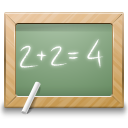
\includegraphics[bb=0 0 18 18]{/data/relax/tags/2.2.0/graphics/oxygen_icons/128x128/categories/applications-education}%
\lthtmlpictureZ
\lthtmlcheckvsize\clearpage}

\stepcounter{subsubsection}
\stepcounter{subsubsection}
\stepcounter{subsubsection}
\stepcounter{subsubsection}
\stepcounter{subsection}
\stepcounter{subsection}
\stepcounter{subsubsection}
\stepcounter{subsubsection}
\stepcounter{subsubsection}
\stepcounter{subsubsection}
\stepcounter{subsubsection}
\stepcounter{subsection}
\stepcounter{subsection}
{\newpage\clearpage
\lthtmlpictureA{tex2html_wrap87987}%

\includegraphics[bb=0 0 18 18]{/data/relax/tags/2.2.0/graphics/oxygen_icons/128x128/actions/edit-select}%
\lthtmlpictureZ
\lthtmlcheckvsize\clearpage}

\stepcounter{subsubsection}
\stepcounter{subsubsection}
\stepcounter{subsubsection}
\stepcounter{subsubsection}
\stepcounter{subsubsection}
\stepcounter{subsection}
\stepcounter{subsection}
\stepcounter{subsubsection}
\stepcounter{subsubsection}
\stepcounter{subsubsection}
\stepcounter{subsubsection}
\stepcounter{subsection}
\stepcounter{subsection}
\stepcounter{subsubsection}
\stepcounter{subsubsection}
\stepcounter{subsubsection}
\stepcounter{subsection}
\stepcounter{subsection}
{\newpage\clearpage
\lthtmlpictureA{tex2html_wrap88011}%

\includegraphics[bb=0 0 18 18]{/data/relax/tags/2.2.0/graphics/relax_icons/128x128/bmrb}%
\lthtmlpictureZ
\lthtmlcheckvsize\clearpage}

{\newpage\clearpage
\lthtmlpictureA{tex2html_wrap88012}%

\includegraphics[bb=0 0 18 18]{/data/relax/tags/2.2.0/graphics/oxygen_icons/128x128/actions/documentation}%
\lthtmlpictureZ
\lthtmlcheckvsize\clearpage}

\stepcounter{subsubsection}
\stepcounter{subsubsection}
\stepcounter{subsubsection}
\stepcounter{subsubsection}
\stepcounter{subsubsection}
\stepcounter{subsection}
\stepcounter{subsection}
\stepcounter{subsubsection}
\stepcounter{subsubsection}
\stepcounter{subsubsection}
\stepcounter{subsubsection}
\stepcounter{subsection}
\stepcounter{subsection}
{\newpage\clearpage
\lthtmlpictureA{tex2html_wrap88057}%

\includegraphics[bb=0 0 18 18]{/data/relax/tags/2.2.0/graphics/oxygen_icons/128x128/actions/document-open}%
\lthtmlpictureZ
\lthtmlcheckvsize\clearpage}

\stepcounter{subsubsection}
\stepcounter{subsubsection}
\stepcounter{subsubsection}
\stepcounter{subsubsection}
\stepcounter{subsection}
\stepcounter{subsection}
{\newpage\clearpage
\lthtmlpictureA{tex2html_wrap88065}%

\includegraphics[bb=0 0 18 18]{/data/relax/tags/2.2.0/graphics/oxygen_icons/128x128/mimetypes/application-x-desktop}%
\lthtmlpictureZ
\lthtmlcheckvsize\clearpage}

\stepcounter{subsubsection}
\stepcounter{subsubsection}
\stepcounter{subsubsection}
\stepcounter{subsubsection}
\stepcounter{subsubsection}
\stepcounter{subsection}
\stepcounter{subsection}
{\newpage\clearpage
\lthtmlpictureA{tex2html_wrap88099}%

\includegraphics[bb=0 0 18 18]{/data/relax/tags/2.2.0/graphics/oxygen_icons/128x128/apps/utilities-terminal}%
\lthtmlpictureZ
\lthtmlcheckvsize\clearpage}

\stepcounter{subsubsection}
\stepcounter{subsubsection}
\stepcounter{subsubsection}
\stepcounter{subsubsection}
\stepcounter{subsubsection}
\stepcounter{subsection}
\stepcounter{subsection}
\stepcounter{subsubsection}
\stepcounter{subsubsection}
\stepcounter{subsubsection}
\stepcounter{subsubsection}
\stepcounter{subsubsection}
\stepcounter{subsection}
\stepcounter{subsection}
\stepcounter{subsubsection}
\stepcounter{subsubsection}
\stepcounter{subsubsection}
\stepcounter{subsubsection}
\stepcounter{subsubsection}
\stepcounter{subsection}
\stepcounter{subsection}
{\newpage\clearpage
\lthtmlpictureA{tex2html_wrap88167}%

\includegraphics[bb=0 0 18 18]{/data/relax/tags/2.2.0/graphics/oxygen_icons/128x128/actions/document-save}%
\lthtmlpictureZ
\lthtmlcheckvsize\clearpage}

\stepcounter{subsubsection}
\stepcounter{subsubsection}
\stepcounter{subsubsection}
\stepcounter{subsubsection}
\stepcounter{subsection}
\stepcounter{subsection}
{\newpage\clearpage
\lthtmlpictureA{tex2html_wrap88174}%
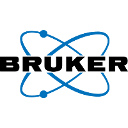
\includegraphics[bb=0 0 18 18]{/data/relax/tags/2.2.0/graphics/relax_icons/128x128/bruker}%
\lthtmlpictureZ
\lthtmlcheckvsize\clearpage}

\stepcounter{subsubsection}
\stepcounter{subsubsection}
\stepcounter{subsubsection}
\stepcounter{subsubsection}
\stepcounter{subsection}
\stepcounter{subsection}
{\newpage\clearpage
\lthtmlpictureA{tex2html_wrap88184}%
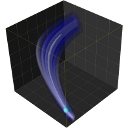
\includegraphics[bb=0 0 18 18]{/data/relax/tags/2.2.0/graphics/relax_icons/128x128/minimise}%
\lthtmlpictureZ
\lthtmlcheckvsize\clearpage}

\stepcounter{subsubsection}
\stepcounter{subsubsection}
\stepcounter{subsubsection}
\stepcounter{subsubsection}
\stepcounter{subsection}
\stepcounter{subsection}
{\newpage\clearpage
\lthtmlpictureA{tex2html_wrap88191}%
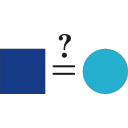
\includegraphics[bb=0 0 18 18]{/data/relax/tags/2.2.0/graphics/relax_icons/128x128/consistency_testing}%
\lthtmlpictureZ
\lthtmlcheckvsize\clearpage}

{\newpage\clearpage
\lthtmlpictureA{tex2html_wrap88192}%

\includegraphics[bb=0 0 18 18]{/data/relax/tags/2.2.0/graphics/relax_icons/128x128/frq}%
\lthtmlpictureZ
\lthtmlcheckvsize\clearpage}

\stepcounter{subsubsection}
\stepcounter{subsubsection}
\stepcounter{subsubsection}
\stepcounter{subsubsection}
\stepcounter{subsubsection}
\stepcounter{subsection}
\stepcounter{subsection}
{\newpage\clearpage
\lthtmlpictureA{tex2html_wrap88204}%

\includegraphics[bb=0 0 18 18]{/data/relax/tags/2.2.0/graphics/oxygen_icons/128x128/actions/list-add-relax-blue}%
\lthtmlpictureZ
\lthtmlcheckvsize\clearpage}

\stepcounter{subsubsection}
\stepcounter{subsubsection}
\stepcounter{subsubsection}
\stepcounter{subsubsection}
\stepcounter{subsubsection}
\stepcounter{subsection}
\stepcounter{subsection}
\stepcounter{subsubsection}
\stepcounter{subsubsection}
\stepcounter{subsubsection}
\stepcounter{subsubsection}
\stepcounter{subsection}
\stepcounter{subsection}
{\newpage\clearpage
\lthtmlpictureA{tex2html_wrap88221}%

\includegraphics[bb=0 0 18 18]{/data/relax/tags/2.2.0/graphics/oxygen_icons/128x128/actions/archive-extract}%
\lthtmlpictureZ
\lthtmlcheckvsize\clearpage}

\stepcounter{subsubsection}
\stepcounter{subsubsection}
\stepcounter{subsubsection}
\stepcounter{subsubsection}
\stepcounter{subsection}
\stepcounter{subsection}
{\newpage\clearpage
\lthtmlpictureA{tex2html_wrap88228}%

\includegraphics[bb=0 0 18 18]{/data/relax/tags/2.2.0/graphics/relax_icons/128x128/spin_grey}%
\lthtmlpictureZ
\lthtmlcheckvsize\clearpage}

\stepcounter{subsubsection}
\stepcounter{subsubsection}
\stepcounter{subsubsection}
\stepcounter{subsubsection}
\stepcounter{subsection}
\stepcounter{subsection}
\stepcounter{subsubsection}
\stepcounter{subsubsection}
\stepcounter{subsubsection}
\stepcounter{subsubsection}
\stepcounter{subsubsection}
\stepcounter{subsubsection}
\stepcounter{subsection}
\stepcounter{subsection}
\stepcounter{subsubsection}
\stepcounter{subsubsection}
\stepcounter{subsubsection}
\stepcounter{subsubsection}
\stepcounter{subsubsection}
\stepcounter{subsubsection}
\stepcounter{subsection}
\stepcounter{subsection}
{\newpage\clearpage
\lthtmlpictureA{tex2html_wrap88368}%

\includegraphics[bb=0 0 18 18]{/data/relax/tags/2.2.0/graphics/oxygen_icons/128x128/actions/system-switch-user}%
\lthtmlpictureZ
\lthtmlcheckvsize\clearpage}

\stepcounter{subsubsection}
\stepcounter{subsubsection}
\stepcounter{subsubsection}
\stepcounter{subsubsection}
\stepcounter{subsubsection}
\stepcounter{subsection}
\stepcounter{subsection}
\stepcounter{subsubsection}
\stepcounter{subsubsection}
\stepcounter{subsubsection}
\stepcounter{subsubsection}
\stepcounter{subsubsection}
\stepcounter{subsubsection}
\stepcounter{subsection}
\stepcounter{subsection}
{\newpage\clearpage
\lthtmlpictureA{tex2html_wrap88386}%
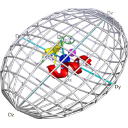
\includegraphics[bb=0 0 18 18]{/data/relax/tags/2.2.0/graphics/relax_icons/128x128/diff_tensor}%
\lthtmlpictureZ
\lthtmlcheckvsize\clearpage}

\stepcounter{subsubsection}
\stepcounter{subsubsection}
\stepcounter{subsubsection}
\stepcounter{subsubsection}
\stepcounter{subsubsection}
\stepcounter{subsection}
\stepcounter{subsection}
\stepcounter{subsubsection}
\stepcounter{subsubsection}
\stepcounter{subsubsection}
\stepcounter{subsection}
\stepcounter{subsection}
\stepcounter{subsubsection}
\stepcounter{subsubsection}
\stepcounter{subsubsection}
\stepcounter{subsection}
\stepcounter{subsection}
\stepcounter{subsubsection}
\stepcounter{subsubsection}
\stepcounter{subsubsection}
\stepcounter{subsubsection}
\stepcounter{subsubsection}
{\newpage\clearpage
\lthtmlinlinemathA{tex2html_wrap_inline88568}%
$ \le$%
\lthtmlinlinemathZ
\lthtmlcheckvsize\clearpage}

{\newpage\clearpage
\lthtmlinlinemathA{tex2html_wrap_inline88604}%
$ \ge$%
\lthtmlinlinemathZ
\lthtmlcheckvsize\clearpage}

\stepcounter{subsubsection}
{\newpage\clearpage
\lthtmlinlinemathA{tex2html_wrap_inline88628}%
$ \delta_{y}^{}$%
\lthtmlinlinemathZ
\lthtmlcheckvsize\clearpage}

{\newpage\clearpage
\lthtmlinlinemathA{tex2html_wrap_inline88632}%
$ \delta_{x}^{}$%
\lthtmlinlinemathZ
\lthtmlcheckvsize\clearpage}

\stepcounter{subsubsection}
\stepcounter{subsubsection}
\stepcounter{subsection}
\stepcounter{subsection}
{\newpage\clearpage
\lthtmlpictureA{tex2html_wrap88938}%
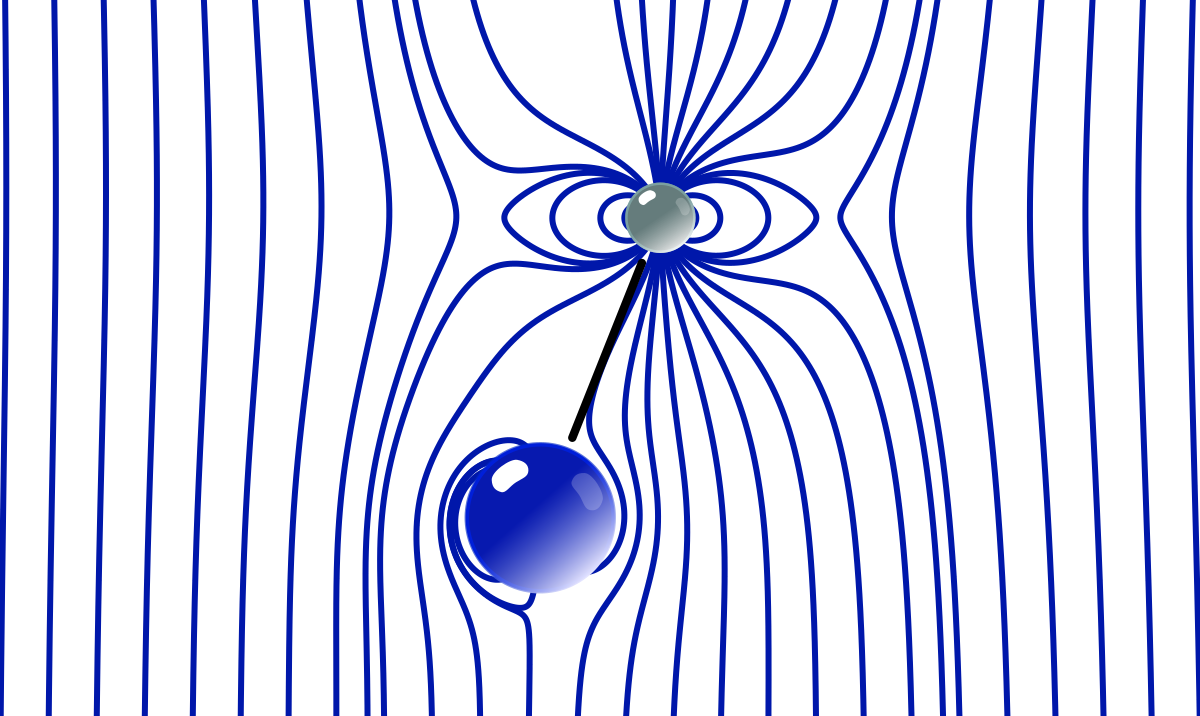
\includegraphics[bb=0 0 18 18]{/data/relax/tags/2.2.0/graphics/relax_icons/128x128/dipole_pair}%
\lthtmlpictureZ
\lthtmlcheckvsize\clearpage}

\stepcounter{subsubsection}
\stepcounter{subsubsection}
\stepcounter{subsubsection}
\stepcounter{subsubsection}
\stepcounter{subsubsection}
\stepcounter{subsection}
\stepcounter{subsection}
\stepcounter{subsubsection}
\stepcounter{subsubsection}
\stepcounter{subsubsection}
\stepcounter{subsubsection}
\stepcounter{subsubsection}
\stepcounter{subsection}
\stepcounter{subsection}
{\newpage\clearpage
\lthtmlpictureA{tex2html_wrap88959}%

\includegraphics[bb=0 0 18 18]{/data/relax/tags/2.2.0/graphics/oxygen_icons/128x128/actions/edit-rename}%
\lthtmlpictureZ
\lthtmlcheckvsize\clearpage}

\stepcounter{subsubsection}
\stepcounter{subsubsection}
\stepcounter{subsubsection}
\stepcounter{subsubsection}
\stepcounter{subsubsection}
\stepcounter{subsection}
\stepcounter{subsection}
\stepcounter{subsubsection}
\stepcounter{subsubsection}
\stepcounter{subsubsection}
\stepcounter{subsubsection}
\stepcounter{subsubsection}
\stepcounter{subsection}
\stepcounter{subsection}
{\newpage\clearpage
\lthtmlpictureA{tex2html_wrap88977}%

\includegraphics[bb=0 0 18 18]{/data/relax/tags/2.2.0/graphics/relax_icons/128x128/opendx}%
\lthtmlpictureZ
\lthtmlcheckvsize\clearpage}

\stepcounter{subsubsection}
\stepcounter{subsubsection}
\stepcounter{subsubsection}
\stepcounter{subsubsection}
\stepcounter{subsection}
\stepcounter{subsection}
{\newpage\clearpage
\lthtmlpictureA{tex2html_wrap88988}%
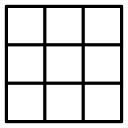
\includegraphics[bb=0 0 18 18]{/data/relax/tags/2.2.0/graphics/relax_icons/128x128/grid_search}%
\lthtmlpictureZ
\lthtmlcheckvsize\clearpage}

\stepcounter{subsubsection}
\stepcounter{subsubsection}
\stepcounter{subsubsection}
\stepcounter{subsubsection}
\stepcounter{subsubsection}
\stepcounter{subsubsection}
\stepcounter{subsubsection}
\stepcounter{subsubsection}
\stepcounter{subsection}
\stepcounter{subsection}
{\newpage\clearpage
\lthtmlpictureA{tex2html_wrap89149}%

\includegraphics[bb=0 0 18 18]{/data/relax/tags/2.2.0/graphics/oxygen_icons/128x128/actions/edit-delete}%
\lthtmlpictureZ
\lthtmlcheckvsize\clearpage}

\stepcounter{subsubsection}
\stepcounter{subsubsection}
\stepcounter{subsubsection}
\stepcounter{subsubsection}
\stepcounter{subsubsection}
\stepcounter{subsubsection}
\stepcounter{subsubsection}
\stepcounter{subsection}
\stepcounter{subsection}
\stepcounter{subsubsection}
\stepcounter{subsubsection}
\stepcounter{subsubsection}
\stepcounter{subsubsection}
\stepcounter{subsection}
\stepcounter{subsection}
{\newpage\clearpage
\lthtmlpictureA{tex2html_wrap89191}%

\includegraphics[bb=0 0 18 18]{/data/relax/tags/2.2.0/graphics/relax_icons/128x128/frame_order}%
\lthtmlpictureZ
\lthtmlcheckvsize\clearpage}

\stepcounter{subsubsection}
\stepcounter{subsubsection}
\stepcounter{subsubsection}
\stepcounter{subsubsection}
\stepcounter{subsection}
\stepcounter{subsection}
\stepcounter{subsubsection}
\stepcounter{subsubsection}
\stepcounter{subsubsection}
\stepcounter{subsubsection}
\stepcounter{subsubsection}
\stepcounter{subsection}
\stepcounter{subsection}
\stepcounter{subsubsection}
\stepcounter{subsubsection}
\stepcounter{subsubsection}
\stepcounter{subsubsection}
\stepcounter{subsubsection}
\stepcounter{subsection}
\stepcounter{subsection}
\stepcounter{subsubsection}
\stepcounter{subsubsection}
\stepcounter{subsubsection}
\stepcounter{subsubsection}
\stepcounter{subsubsection}
\stepcounter{subsection}
\stepcounter{subsection}
\stepcounter{subsubsection}
\stepcounter{subsubsection}
\stepcounter{subsubsection}
\stepcounter{subsubsection}
\stepcounter{subsubsection}
\stepcounter{subsection}
\stepcounter{subsection}
\stepcounter{subsubsection}
\stepcounter{subsubsection}
\stepcounter{subsubsection}
\stepcounter{subsubsection}
\stepcounter{subsection}
\stepcounter{subsection}
{\newpage\clearpage
\lthtmlpictureA{tex2html_wrap89266}%

\includegraphics[bb=0 0 18 18]{/data/relax/tags/2.2.0/graphics/relax_icons/128x128/grace_icon}%
\lthtmlpictureZ
\lthtmlcheckvsize\clearpage}

\stepcounter{subsubsection}
\stepcounter{subsubsection}
\stepcounter{subsubsection}
\stepcounter{subsubsection}
\stepcounter{subsubsection}
\stepcounter{subsection}
\stepcounter{subsection}
\stepcounter{subsubsection}
\stepcounter{subsubsection}
\stepcounter{subsubsection}
\stepcounter{subsubsection}
\stepcounter{subsubsection}
\stepcounter{subsubsection}
\stepcounter{subsubsection}
\stepcounter{subsubsection}
\stepcounter{subsubsection}
{\newpage\clearpage
\lthtmlinlinemathA{tex2html_wrap_inline89362}%
$ \omega_{X}^{}$%
\lthtmlinlinemathZ
\lthtmlcheckvsize\clearpage}

{\newpage\clearpage
\lthtmlinlinemathA{tex2html_wrap_inline89364}%
$ \omega_{H}^{}$%
\lthtmlinlinemathZ
\lthtmlcheckvsize\clearpage}

\stepcounter{subsubsection}
\stepcounter{subsubsection}
\stepcounter{subsubsection}
\stepcounter{subsection}
\stepcounter{subsection}
\stepcounter{subsubsection}
\stepcounter{subsubsection}
\stepcounter{subsubsection}
\stepcounter{subsubsection}
\stepcounter{subsection}
\stepcounter{subsection}
\stepcounter{subsubsection}
\stepcounter{subsubsection}
\stepcounter{subsubsection}
\stepcounter{subsubsection}
\stepcounter{subsubsection}
\stepcounter{subsection}
\stepcounter{subsection}
\stepcounter{subsubsection}
\stepcounter{subsubsection}
\stepcounter{subsubsection}
\stepcounter{subsubsection}
\stepcounter{subsubsection}
\stepcounter{subsection}
\stepcounter{subsection}
{\newpage\clearpage
\lthtmlpictureA{tex2html_wrap89439}%
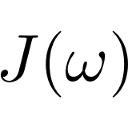
\includegraphics[bb=0 0 18 18]{/data/relax/tags/2.2.0/graphics/relax_icons/128x128/jw_mapping}%
\lthtmlpictureZ
\lthtmlcheckvsize\clearpage}

\stepcounter{subsubsection}
\stepcounter{subsubsection}
\stepcounter{subsubsection}
\stepcounter{subsubsection}
\stepcounter{subsubsection}
\stepcounter{subsection}
\stepcounter{subsection}
\stepcounter{subsubsection}
\stepcounter{subsubsection}
\stepcounter{subsubsection}
\stepcounter{subsubsection}
\stepcounter{subsubsection}
\stepcounter{subsubsection}
\stepcounter{subsubsection}
\stepcounter{subsubsection}
\stepcounter{subsection}
\stepcounter{subsection}
{\newpage\clearpage
\lthtmlpictureA{tex2html_wrap89607}%
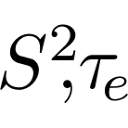
\includegraphics[bb=0 0 18 18]{/data/relax/tags/2.2.0/graphics/relax_icons/128x128/model-free}%
\lthtmlpictureZ
\lthtmlcheckvsize\clearpage}

\stepcounter{subsubsection}
\stepcounter{subsubsection}
\stepcounter{subsubsection}
\stepcounter{subsubsection}
\stepcounter{subsubsection}
\stepcounter{subsubsection}
\stepcounter{subsubsection}
\stepcounter{subsubsection}
\stepcounter{subsection}
\stepcounter{subsection}
\stepcounter{subsubsection}
\stepcounter{subsubsection}
\stepcounter{subsubsection}
\stepcounter{subsubsection}
\stepcounter{subsection}
\stepcounter{subsection}
\stepcounter{subsubsection}
\stepcounter{subsubsection}
\stepcounter{subsubsection}
\stepcounter{subsubsection}
\stepcounter{subsubsection}
\stepcounter{subsection}
\stepcounter{subsection}
\stepcounter{subsubsection}
\stepcounter{subsubsection}
\stepcounter{subsubsection}
\stepcounter{subsubsection}
\stepcounter{subsubsection}
\stepcounter{subsubsection}
\stepcounter{subsubsection}
\stepcounter{subsubsection}
\stepcounter{subsection}
\stepcounter{subsection}
{\newpage\clearpage
\lthtmlpictureA{tex2html_wrap90157}%
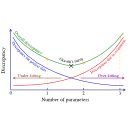
\includegraphics[bb=0 0 18 18]{/data/relax/tags/2.2.0/graphics/relax_icons/128x128/discrepancy_curve}%
\lthtmlpictureZ
\lthtmlcheckvsize\clearpage}

\stepcounter{subsubsection}
\stepcounter{subsubsection}
\stepcounter{subsubsection}
\stepcounter{subsubsection}
\stepcounter{subsubsection}
\stepcounter{subsection}
\stepcounter{subsection}
{\newpage\clearpage
\lthtmlpictureA{tex2html_wrap90174}%
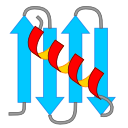
\includegraphics[bb=0 0 18 18]{/data/relax/tags/2.2.0/graphics/relax_icons/128x128/molecule}%
\lthtmlpictureZ
\lthtmlcheckvsize\clearpage}

\stepcounter{subsubsection}
\stepcounter{subsubsection}
\stepcounter{subsubsection}
\stepcounter{subsubsection}
\stepcounter{subsubsection}
\stepcounter{subsubsection}
\stepcounter{subsection}
\stepcounter{subsection}
\stepcounter{subsubsection}
\stepcounter{subsubsection}
\stepcounter{subsubsection}
\stepcounter{subsubsection}
\stepcounter{subsubsection}
\stepcounter{subsection}
\stepcounter{subsection}
\stepcounter{subsubsection}
\stepcounter{subsubsection}
\stepcounter{subsubsection}
\stepcounter{subsubsection}
\stepcounter{subsubsection}
\stepcounter{subsection}
\stepcounter{subsection}
\stepcounter{subsubsection}
\stepcounter{subsubsection}
\stepcounter{subsubsection}
\stepcounter{subsubsection}
\stepcounter{subsection}
\stepcounter{subsection}
\stepcounter{subsubsection}
\stepcounter{subsubsection}
\stepcounter{subsubsection}
\stepcounter{subsubsection}
\stepcounter{subsubsection}
\stepcounter{subsubsection}
\stepcounter{subsection}
\stepcounter{subsection}
\stepcounter{subsubsection}
\stepcounter{subsubsection}
\stepcounter{subsubsection}
\stepcounter{subsubsection}
\stepcounter{subsubsection}
\stepcounter{subsubsection}
\stepcounter{subsection}
\stepcounter{subsection}
{\newpage\clearpage
\lthtmlpictureA{tex2html_wrap90240}%

\includegraphics[bb=0 0 18 18]{/data/relax/tags/2.2.0/graphics/relax_icons/128x128/molmol}%
\lthtmlpictureZ
\lthtmlcheckvsize\clearpage}

\stepcounter{subsubsection}
\stepcounter{subsubsection}
\stepcounter{subsubsection}
\stepcounter{subsection}
\stepcounter{subsection}
\stepcounter{subsubsection}
\stepcounter{subsubsection}
\stepcounter{subsubsection}
\stepcounter{subsubsection}
\stepcounter{subsubsection}
\stepcounter{subsection}
\stepcounter{subsection}
\stepcounter{subsubsection}
\stepcounter{subsubsection}
\stepcounter{subsubsection}
\stepcounter{subsubsection}
\stepcounter{subsubsection}
\stepcounter{subsubsection}
{\newpage\clearpage
\lthtmlfigureA{tablestar21020}%
\begin{table*}\begin{scriptsize}
\begin{center}

\begin{tabularx}{\textwidth}{llX}
\\[-5pt]
\toprule
Data type & String & Description \\
\midrule
$S^2$. & 's2' & The standard model-free order parameter, equal to $S^2_f$.S2s for the two timescale models.  The default colour gradient starts at 'yellow' and ends at 'red'. \\
$S^2_f$. & 's2f' & The order parameter of the faster of two internal motions.  Residues which are described by model-free models m1 to m4, the single timescale models, are illustrated as white neon bonds.  The default colour gradient is the same as that for the $S^2$\  data type. \\
$S^2_s$. & 's2s' & The order parameter of the slower of two internal motions.  This functions exactly as $S^2_f$\  except that $S^2_s$\  is plotted instead. \\
Amplitude of fast motions. & 'amp\_fast' & Model independent display of the amplite of fast motions.  For residues described by model-free models m5 to m8, the value plotted is that of $S^2_f$.  However, for residues described by models m1 to m4, what is shown is dependent on the timescale of the motions.  This is because these single timescale models can, at times, be perfect approximations to the more complex two timescale models.  Hence if $\tau_e$\  is less than 200 ps, $S^2$\  is plotted.  Otherwise the peptide bond is coloured white.  The default colour gradient  is the same as that for $S^2$. \\
Amplitude of slow motions. & 'amp\_slow' & Model independent display of the amplite of slow motions, arbitrarily defined as motions slower than 200 ps.  For residues described by model-free models m5 to m8, the order parameter $S^2$\  is plotted if $\tau_s$\  $>$\  200 ps.  For models m1 to m4, $S^2$\  is plotted if $\tau_e$\  $>$\  200 ps.  The default colour gradient is the same as that for $S^2$. \\
$\tau_e$. & 'te' & The correlation time, $\tau_e$.  The default colour gradient starts at 'turquoise' and ends at 'blue'. \\
$\tau_f$. & 'tf' & The correlation time, $\tau_f$.  The default colour gradient is the same as that of $\tau_e$. \\
$\tau_s$. & 'ts' & The correlation time, $\tau_s$.  The default colour gradient starts at 'blue' and ends at 'black'. \\
Timescale of fast motions & 'time\_fast' & Model independent display of the timescale of fast motions.  For models m5 to m8, only the parameter $\tau_f$\  is plotted.  For models m2 and m4, the parameter $\tau_e$\  is plotted only if it is less than 200 ps.  All other residues are assumed to have a correlation time of zero.  The default colour gradient is the same as that of $\tau_e$. \\
Timescale of slow motions & 'time\_slow' & Model independent display of the timescale of slow motions.  For models m5 to m8, only the parameter $\tau_s$\  is plotted.  For models m2 and m4, the parameter $\tau_e$\  is plotted only if it is greater than 200 ps.  All other residues are coloured white.  The default colour gradient is the same as that of $\tau_s$. \\
Chemical exchange & 'rex' & The chemical exchange, $R_{ex}$.  Residues which experience no chemical exchange are coloured white.  The default colour gradient starts at 'yellow' and finishes at 'red'. \\
\bottomrule
\\[-5pt]
\end{tabularx}
\end{center}
\end{scriptsize}
\end{table*}%
\lthtmlfigureZ
\lthtmlcheckvsize\clearpage}

\stepcounter{subsubsection}
\stepcounter{subsubsection}
\stepcounter{subsubsection}
\stepcounter{subsection}
\stepcounter{subsection}
\stepcounter{subsubsection}
\stepcounter{subsubsection}
\stepcounter{subsubsection}
\stepcounter{subsubsection}
\stepcounter{subsubsection}
\stepcounter{subsection}
\stepcounter{subsection}
\stepcounter{subsubsection}
\stepcounter{subsubsection}
\stepcounter{subsubsection}
\stepcounter{subsubsection}
\stepcounter{subsubsection}
\stepcounter{subsubsection}
\stepcounter{subsubsection}
\stepcounter{subsubsection}
\stepcounter{subsubsection}
\stepcounter{subsection}
\stepcounter{subsection}
\stepcounter{subsubsection}
\stepcounter{subsubsection}
\stepcounter{subsubsection}
\stepcounter{subsubsection}
\stepcounter{subsection}
\stepcounter{subsection}
\stepcounter{subsubsection}
\stepcounter{subsubsection}
\stepcounter{subsubsection}
\stepcounter{subsubsection}
\stepcounter{subsection}
\stepcounter{subsection}
\stepcounter{subsubsection}
\stepcounter{subsubsection}
\stepcounter{subsubsection}
\stepcounter{subsubsection}
\stepcounter{subsection}
\stepcounter{subsection}
{\newpage\clearpage
\lthtmlpictureA{tex2html_wrap92722}%

\includegraphics[bb=0 0 18 18]{/data/relax/tags/2.2.0/graphics/oxygen_icons/128x128/actions/roll-relax-blue}%
\lthtmlpictureZ
\lthtmlcheckvsize\clearpage}

\stepcounter{subsubsection}
\stepcounter{subsubsection}
\stepcounter{subsubsection}
\stepcounter{subsubsection}
\stepcounter{subsubsection}
\stepcounter{subsection}
\stepcounter{subsection}
\stepcounter{subsubsection}
\stepcounter{subsubsection}
\stepcounter{subsubsection}
\stepcounter{subsubsection}
\stepcounter{subsection}
\stepcounter{subsection}
\stepcounter{subsubsection}
\stepcounter{subsubsection}
\stepcounter{subsubsection}
\stepcounter{subsubsection}
\stepcounter{subsection}
\stepcounter{subsection}
{\newpage\clearpage
\lthtmlpictureA{tex2html_wrap92775}%

\includegraphics[bb=0 0 18 18]{/data/relax/tags/2.2.0/graphics/oxygen_icons/128x128/actions/dialog-cancel}%
\lthtmlpictureZ
\lthtmlcheckvsize\clearpage}

\stepcounter{subsubsection}
\stepcounter{subsubsection}
\stepcounter{subsubsection}
\stepcounter{subsubsection}
\stepcounter{subsection}
\stepcounter{subsection}
{\newpage\clearpage
\lthtmlpictureA{tex2html_wrap92792}%

\includegraphics[bb=0 0 18 18]{/data/relax/tags/2.2.0/graphics/oxygen_icons/128x128/actions/dialog-ok}%
\lthtmlpictureZ
\lthtmlcheckvsize\clearpage}

\stepcounter{subsubsection}
\stepcounter{subsubsection}
\stepcounter{subsubsection}
\stepcounter{subsubsection}
\stepcounter{subsection}
\stepcounter{subsection}
{\newpage\clearpage
\lthtmlpictureA{tex2html_wrap92809}%

\includegraphics[bb=0 0 18 18]{/data/relax/tags/2.2.0/graphics/oxygen_icons/128x128/actions/document-edit}%
\lthtmlpictureZ
\lthtmlcheckvsize\clearpage}

\stepcounter{subsubsection}
\stepcounter{subsubsection}
\stepcounter{subsubsection}
\stepcounter{subsubsection}
\stepcounter{subsubsection}
\stepcounter{subsection}
\stepcounter{subsection}
{\newpage\clearpage
\lthtmlpictureA{tex2html_wrap92826}%

\includegraphics[bb=0 0 18 18]{/data/relax/tags/2.2.0/graphics/relax_icons/128x128/n_state_model}%
\lthtmlpictureZ
\lthtmlcheckvsize\clearpage}

\stepcounter{subsubsection}
\stepcounter{subsubsection}
\stepcounter{subsubsection}
\stepcounter{subsubsection}
\stepcounter{subsubsection}
\stepcounter{subsection}
\stepcounter{subsection}
\stepcounter{subsubsection}
\stepcounter{subsubsection}
\stepcounter{subsubsection}
\stepcounter{subsubsection}
\stepcounter{subsection}
\stepcounter{subsection}
\stepcounter{subsubsection}
\stepcounter{subsubsection}
\stepcounter{subsubsection}
\stepcounter{subsubsection}
\stepcounter{subsection}
\stepcounter{subsection}
\stepcounter{subsubsection}
\stepcounter{subsubsection}
\stepcounter{subsubsection}
\stepcounter{subsubsection}
\stepcounter{subsubsection}
\stepcounter{subsection}
\stepcounter{subsection}
\stepcounter{subsubsection}
\stepcounter{subsubsection}
\stepcounter{subsubsection}
\stepcounter{subsubsection}
\stepcounter{subsubsection}
\stepcounter{subsection}
\stepcounter{subsection}
\stepcounter{subsubsection}
\stepcounter{subsubsection}
\stepcounter{subsubsection}
\stepcounter{subsubsection}
\stepcounter{subsubsection}
\stepcounter{subsection}
\stepcounter{subsection}
{\newpage\clearpage
\lthtmlpictureA{tex2html_wrap92884}%
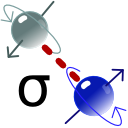
\includegraphics[bb=0 0 18 18]{/data/relax/tags/2.2.0/graphics/relax_icons/128x128/noe}%
\lthtmlpictureZ
\lthtmlcheckvsize\clearpage}

\stepcounter{subsubsection}
\stepcounter{subsubsection}
\stepcounter{subsubsection}
\stepcounter{subsubsection}
\stepcounter{subsubsection}
\stepcounter{subsection}
\stepcounter{subsection}
\stepcounter{subsubsection}
\stepcounter{subsubsection}
\stepcounter{subsubsection}
\stepcounter{subsubsection}
\stepcounter{subsection}
\stepcounter{subsection}
{\newpage\clearpage
\lthtmlpictureA{tex2html_wrap92905}%
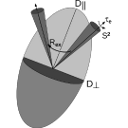
\includegraphics[bb=0 0 18 18]{/data/relax/tags/2.2.0/graphics/relax_icons/128x128/modelfree4}%
\lthtmlpictureZ
\lthtmlcheckvsize\clearpage}

\stepcounter{subsubsection}
\stepcounter{subsubsection}
\stepcounter{subsubsection}
\stepcounter{subsubsection}
\stepcounter{subsection}
\stepcounter{subsection}
\stepcounter{subsubsection}
\stepcounter{subsubsection}
\stepcounter{subsubsection}
\stepcounter{subsubsection}
\stepcounter{subsection}
\stepcounter{subsection}
\stepcounter{subsubsection}
\stepcounter{subsubsection}
\stepcounter{subsubsection}
\stepcounter{subsubsection}
\stepcounter{subsection}
\stepcounter{subsection}
\stepcounter{subsubsection}
\stepcounter{subsubsection}
\stepcounter{subsubsection}
\stepcounter{subsubsection}
\stepcounter{subsubsection}
\stepcounter{subsection}
\stepcounter{subsection}
\stepcounter{subsubsection}
\stepcounter{subsubsection}
\stepcounter{subsubsection}
\stepcounter{subsubsection}
\stepcounter{subsection}
\stepcounter{subsection}
\stepcounter{subsubsection}
\stepcounter{subsubsection}
\stepcounter{subsubsection}
\stepcounter{subsubsection}
\stepcounter{subsubsection}
\stepcounter{subsection}
\stepcounter{subsection}
\stepcounter{subsubsection}
\stepcounter{subsubsection}
\stepcounter{subsubsection}
\stepcounter{subsubsection}
\stepcounter{subsubsection}
\stepcounter{subsection}
\stepcounter{subsection}
\stepcounter{subsubsection}
\stepcounter{subsubsection}
\stepcounter{subsubsection}
\stepcounter{subsubsection}
\stepcounter{subsubsection}
\stepcounter{subsection}
\stepcounter{subsection}
\stepcounter{subsubsection}
\stepcounter{subsubsection}
\stepcounter{subsubsection}
\stepcounter{subsubsection}
\stepcounter{subsubsection}
\stepcounter{subsection}
\stepcounter{subsection}
\stepcounter{subsubsection}
\stepcounter{subsubsection}
\stepcounter{subsubsection}
\stepcounter{subsubsection}
\stepcounter{subsubsection}
\stepcounter{subsection}
\stepcounter{subsection}
\stepcounter{subsubsection}
\stepcounter{subsubsection}
\stepcounter{subsubsection}
\stepcounter{subsubsection}
\stepcounter{subsubsection}
\stepcounter{subsection}
\stepcounter{subsection}
\stepcounter{subsubsection}
\stepcounter{subsubsection}
\stepcounter{subsubsection}
\stepcounter{subsubsection}
\stepcounter{subsection}
\stepcounter{subsection}
\stepcounter{subsubsection}
\stepcounter{subsubsection}
\stepcounter{subsubsection}
\stepcounter{subsubsection}
\stepcounter{subsection}
\stepcounter{subsection}
\stepcounter{subsubsection}
\stepcounter{subsubsection}
\stepcounter{subsubsection}
\stepcounter{subsubsection}
\stepcounter{subsection}
\stepcounter{subsection}
\stepcounter{subsubsection}
\stepcounter{subsubsection}
\stepcounter{subsubsection}
\stepcounter{subsubsection}
\stepcounter{subsection}
\stepcounter{subsection}
{\newpage\clearpage
\lthtmlpictureA{tex2html_wrap93057}%
\includegraphics[bb=0 0 18 18]{/data/relax/tags/2.2.0/graphics/relax_icons/128x128/pipe}%
\lthtmlpictureZ
\lthtmlcheckvsize\clearpage}

{\newpage\clearpage
\lthtmlpictureA{tex2html_wrap93058}%
\includegraphics[bb=0 0 18 18]{/data/relax/tags/2.2.0/graphics/relax_icons/128x128/pipe_bundle}%
\lthtmlpictureZ
\lthtmlcheckvsize\clearpage}

\stepcounter{subsubsection}
\stepcounter{subsubsection}
\stepcounter{subsubsection}
\stepcounter{subsubsection}
\stepcounter{subsubsection}
\stepcounter{subsection}
\stepcounter{subsection}
\stepcounter{subsubsection}
\stepcounter{subsubsection}
\stepcounter{subsubsection}
\stepcounter{subsubsection}
\stepcounter{subsubsection}
\stepcounter{subsection}
\stepcounter{subsection}
\stepcounter{subsubsection}
\stepcounter{subsubsection}
\stepcounter{subsubsection}
\stepcounter{subsubsection}
\stepcounter{subsubsection}
\stepcounter{subsection}
\stepcounter{subsection}
\stepcounter{subsubsection}
\stepcounter{subsubsection}
\stepcounter{subsubsection}
\stepcounter{subsubsection}
\stepcounter{subsubsection}
\stepcounter{subsection}
\stepcounter{subsection}
\stepcounter{subsubsection}
\stepcounter{subsubsection}
\stepcounter{subsubsection}
\stepcounter{subsection}
\stepcounter{subsection}
\stepcounter{subsubsection}
\stepcounter{subsubsection}
\stepcounter{subsubsection}
\stepcounter{subsubsection}
\stepcounter{subsection}
\stepcounter{subsection}
\stepcounter{subsubsection}
\stepcounter{subsubsection}
\stepcounter{subsubsection}
\stepcounter{subsection}
\stepcounter{subsection}
{\newpage\clearpage
\lthtmlpictureA{tex2html_wrap93137}%
\includegraphics[bb=0 0 18 18]{/data/relax/tags/2.2.0/graphics/relax_icons/128x128/pipe_hybrid}%
\lthtmlpictureZ
\lthtmlcheckvsize\clearpage}

\stepcounter{subsubsection}
\stepcounter{subsubsection}
\stepcounter{subsubsection}
\stepcounter{subsubsection}
\stepcounter{subsubsection}
\stepcounter{subsection}
\stepcounter{subsection}
\stepcounter{subsubsection}
\stepcounter{subsubsection}
\stepcounter{subsubsection}
\stepcounter{subsubsection}
\stepcounter{subsubsection}
\stepcounter{subsection}
\stepcounter{subsection}
{\newpage\clearpage
\lthtmlpictureA{tex2html_wrap93154}%
\includegraphics[bb=0 0 18 18]{/data/relax/tags/2.2.0/graphics/relax_icons/128x128/pymol_icon}%
\lthtmlpictureZ
\lthtmlcheckvsize\clearpage}

\stepcounter{subsubsection}
\stepcounter{subsubsection}
\stepcounter{subsubsection}
\stepcounter{subsubsection}
\stepcounter{subsection}
\stepcounter{subsection}
\stepcounter{subsubsection}
\stepcounter{subsubsection}
\stepcounter{subsubsection}
\stepcounter{subsection}
\stepcounter{subsection}
\stepcounter{subsubsection}
\stepcounter{subsubsection}
\stepcounter{subsubsection}
\stepcounter{subsubsection}
\stepcounter{subsubsection}
\stepcounter{subsection}
\stepcounter{subsection}
\stepcounter{subsubsection}
\stepcounter{subsubsection}
\stepcounter{subsubsection}
\stepcounter{subsubsection}
\stepcounter{subsection}
\stepcounter{subsection}
\stepcounter{subsubsection}
\stepcounter{subsubsection}
\stepcounter{subsubsection}
\stepcounter{subsubsection}
\stepcounter{subsubsection}
\stepcounter{subsubsection}
\stepcounter{subsubsection}
\stepcounter{subsubsection}
\stepcounter{subsubsection}
\stepcounter{subsection}
\stepcounter{subsection}
\stepcounter{subsubsection}
\stepcounter{subsubsection}
\stepcounter{subsubsection}
\stepcounter{subsubsection}
\stepcounter{subsubsection}
\stepcounter{subsection}
\stepcounter{subsection}
\stepcounter{subsubsection}
\stepcounter{subsubsection}
\stepcounter{subsubsection}
\stepcounter{subsubsection}
\stepcounter{subsubsection}
\stepcounter{subsubsection}
\stepcounter{subsubsection}
\stepcounter{subsubsection}
\stepcounter{subsubsection}
\stepcounter{subsection}
\stepcounter{subsection}
\stepcounter{subsubsection}
\stepcounter{subsubsection}
\stepcounter{subsubsection}
\stepcounter{subsubsection}
\stepcounter{subsection}
\stepcounter{subsection}
\stepcounter{subsubsection}
\stepcounter{subsubsection}
\stepcounter{subsubsection}
\stepcounter{subsubsection}
\stepcounter{subsection}
\stepcounter{subsection}
\stepcounter{subsubsection}
\stepcounter{subsubsection}
\stepcounter{subsubsection}
\stepcounter{subsubsection}
\stepcounter{subsection}
\stepcounter{subsection}
\stepcounter{subsubsection}
\stepcounter{subsubsection}
\stepcounter{subsubsection}
\stepcounter{subsubsection}
\stepcounter{subsection}
\stepcounter{subsection}
\stepcounter{subsubsection}
\stepcounter{subsubsection}
\stepcounter{subsubsection}
\stepcounter{subsubsection}
\stepcounter{subsubsection}
\stepcounter{subsection}
\stepcounter{subsection}
\stepcounter{subsubsection}
\stepcounter{subsubsection}
\stepcounter{subsubsection}
\stepcounter{subsubsection}
\stepcounter{subsubsection}
\stepcounter{subsection}
\stepcounter{subsection}
\stepcounter{subsubsection}
\stepcounter{subsubsection}
\stepcounter{subsubsection}
\stepcounter{subsubsection}
\stepcounter{subsubsection}
\stepcounter{subsection}
\stepcounter{subsection}
\stepcounter{subsubsection}
\stepcounter{subsubsection}
\stepcounter{subsubsection}
\stepcounter{subsubsection}
\stepcounter{subsubsection}
\stepcounter{subsection}
\stepcounter{subsection}
\stepcounter{subsubsection}
\stepcounter{subsubsection}
\stepcounter{subsubsection}
\stepcounter{subsubsection}
\stepcounter{subsubsection}
\stepcounter{subsection}
\stepcounter{subsection}
\stepcounter{subsubsection}
\stepcounter{subsubsection}
\stepcounter{subsubsection}
\stepcounter{subsubsection}
\stepcounter{subsubsection}
\stepcounter{subsection}
\stepcounter{subsection}
\stepcounter{subsubsection}
\stepcounter{subsubsection}
\stepcounter{subsubsection}
\stepcounter{subsubsection}
\stepcounter{subsection}
\stepcounter{subsection}
\stepcounter{subsubsection}
\stepcounter{subsubsection}
\stepcounter{subsubsection}
\stepcounter{subsubsection}
\stepcounter{subsection}
\stepcounter{subsection}
\stepcounter{subsubsection}
\stepcounter{subsubsection}
\stepcounter{subsubsection}
\stepcounter{subsubsection}
\stepcounter{subsection}
\stepcounter{subsection}
{\newpage\clearpage
\lthtmlpictureA{tex2html_wrap93376}%
\includegraphics[bb=0 0 18 18]{/data/relax/tags/2.2.0/graphics/relax_icons/128x128/fid}%
\lthtmlpictureZ
\lthtmlcheckvsize\clearpage}

\stepcounter{subsubsection}
\stepcounter{subsubsection}
\stepcounter{subsubsection}
\stepcounter{subsubsection}
\stepcounter{subsection}
\stepcounter{subsection}
\stepcounter{subsubsection}
\stepcounter{subsubsection}
\stepcounter{subsubsection}
\stepcounter{subsubsection}
\stepcounter{subsubsection}
\stepcounter{subsection}
\stepcounter{subsection}
\stepcounter{subsubsection}
\stepcounter{subsubsection}
\stepcounter{subsubsection}
\stepcounter{subsubsection}
\stepcounter{subsubsection}
\stepcounter{subsection}
\stepcounter{subsection}
\stepcounter{subsubsection}
\stepcounter{subsubsection}
\stepcounter{subsubsection}
\stepcounter{subsubsection}
\stepcounter{subsubsection}
\stepcounter{subsection}
\stepcounter{subsection}
\stepcounter{subsubsection}
\stepcounter{subsubsection}
\stepcounter{subsubsection}
\stepcounter{subsubsection}
\stepcounter{subsection}
\stepcounter{subsection}
\stepcounter{subsubsection}
\stepcounter{subsubsection}
\stepcounter{subsubsection}
\stepcounter{subsubsection}
\stepcounter{subsection}
\stepcounter{subsection}
\stepcounter{subsubsection}
\stepcounter{subsubsection}
\stepcounter{subsubsection}
\stepcounter{subsubsection}
\stepcounter{subsubsection}
\stepcounter{subsection}
\stepcounter{subsection}
{\newpage\clearpage
\lthtmlpictureA{tex2html_wrap93442}%
\includegraphics[bb=0 0 18 18]{/data/relax/tags/2.2.0/graphics/oxygen_icons/128x128/status/weather-clear}%
\lthtmlpictureZ
\lthtmlcheckvsize\clearpage}

\stepcounter{subsubsection}
\stepcounter{subsubsection}
\stepcounter{subsubsection}
\stepcounter{subsubsection}
\stepcounter{subsection}
\stepcounter{subsection}
\stepcounter{subsubsection}
\stepcounter{subsubsection}
\stepcounter{subsubsection}
\stepcounter{subsubsection}
\stepcounter{subsection}
\stepcounter{subsection}
\stepcounter{subsubsection}
\stepcounter{subsubsection}
\stepcounter{subsubsection}
\stepcounter{subsubsection}
\stepcounter{subsection}
\stepcounter{subsection}
\stepcounter{subsubsection}
\stepcounter{subsubsection}
\stepcounter{subsubsection}
\stepcounter{subsubsection}
\stepcounter{subsection}
\stepcounter{subsection}
{\newpage\clearpage
\lthtmlpictureA{tex2html_wrap93495}%
\includegraphics[bb=0 0 18 18]{/data/relax/tags/2.2.0/graphics/relax_icons/128x128/relax_fit}%
\lthtmlpictureZ
\lthtmlcheckvsize\clearpage}

{\newpage\clearpage
\lthtmlpictureA{tex2html_wrap93496}%
\includegraphics[bb=0 0 18 18]{/data/relax/tags/2.2.0/graphics/oxygen_icons/128x128/actions/chronometer}%
\lthtmlpictureZ
\lthtmlcheckvsize\clearpage}

\stepcounter{subsubsection}
\stepcounter{subsubsection}
\stepcounter{subsubsection}
\stepcounter{subsubsection}
\stepcounter{subsection}
\stepcounter{subsection}
\stepcounter{subsubsection}
\stepcounter{subsubsection}
\stepcounter{subsubsection}
\stepcounter{subsubsection}
\stepcounter{subsection}
\stepcounter{subsection}
{\newpage\clearpage
\lthtmlpictureA{tex2html_wrap93513}%
\includegraphics[bb=0 0 18 18]{/data/relax/tags/2.2.0/graphics/oxygen_icons/128x128/actions/dialog-close}%
\lthtmlpictureZ
\lthtmlcheckvsize\clearpage}

\stepcounter{subsubsection}
\stepcounter{subsubsection}
\stepcounter{subsubsection}
\stepcounter{subsection}
\stepcounter{subsection}
{\newpage\clearpage
\lthtmlpictureA{tex2html_wrap93519}%
\includegraphics[bb=0 0 18 18]{/data/relax/tags/2.2.0/graphics/relax_icons/128x128/residue}%
\lthtmlpictureZ
\lthtmlcheckvsize\clearpage}

\stepcounter{subsubsection}
\stepcounter{subsubsection}
\stepcounter{subsubsection}
\stepcounter{subsubsection}
\stepcounter{subsubsection}
\stepcounter{subsection}
\stepcounter{subsection}
\stepcounter{subsubsection}
\stepcounter{subsubsection}
\stepcounter{subsubsection}
\stepcounter{subsubsection}
\stepcounter{subsubsection}
\stepcounter{subsection}
\stepcounter{subsection}
\stepcounter{subsubsection}
\stepcounter{subsubsection}
\stepcounter{subsubsection}
\stepcounter{subsubsection}
\stepcounter{subsubsection}
\stepcounter{subsection}
\stepcounter{subsection}
\stepcounter{subsubsection}
\stepcounter{subsubsection}
\stepcounter{subsubsection}
\stepcounter{subsubsection}
\stepcounter{subsubsection}
\stepcounter{subsection}
\stepcounter{subsection}
\stepcounter{subsubsection}
\stepcounter{subsubsection}
\stepcounter{subsubsection}
\stepcounter{subsubsection}
\stepcounter{subsubsection}
\stepcounter{subsubsection}
\stepcounter{subsection}
\stepcounter{subsection}
\stepcounter{subsubsection}
\stepcounter{subsubsection}
\stepcounter{subsubsection}
\stepcounter{subsubsection}
\stepcounter{subsubsection}
\stepcounter{subsubsection}
\stepcounter{subsection}
\stepcounter{subsection}
{\newpage\clearpage
\lthtmlpictureA{tex2html_wrap93575}%
\includegraphics[bb=0 0 18 18]{/data/relax/tags/2.2.0/graphics/relax_icons/128x128/relax}%
\lthtmlpictureZ
\lthtmlcheckvsize\clearpage}

\stepcounter{subsubsection}
\stepcounter{subsubsection}
\stepcounter{subsubsection}
\stepcounter{subsection}
\stepcounter{subsection}
\stepcounter{subsubsection}
\stepcounter{subsubsection}
\stepcounter{subsubsection}
\stepcounter{subsubsection}
\stepcounter{subsection}
\stepcounter{subsection}
\stepcounter{subsubsection}
\stepcounter{subsubsection}
\stepcounter{subsubsection}
\stepcounter{subsubsection}
\stepcounter{subsection}
\stepcounter{subsection}
\stepcounter{subsubsection}
\stepcounter{subsubsection}
\stepcounter{subsubsection}
\stepcounter{subsubsection}
\stepcounter{subsection}
\stepcounter{subsection}
{\newpage\clearpage
\lthtmlpictureA{tex2html_wrap93608}%
\includegraphics[bb=0 0 18 18]{/data/relax/tags/2.2.0/graphics/relax_icons/128x128/spin}%
\lthtmlpictureZ
\lthtmlcheckvsize\clearpage}

\stepcounter{subsubsection}
\stepcounter{subsubsection}
\stepcounter{subsubsection}
\stepcounter{subsubsection}
\stepcounter{subsection}
\stepcounter{subsection}
\stepcounter{subsubsection}
\stepcounter{subsubsection}
\stepcounter{subsubsection}
\stepcounter{subsubsection}
\stepcounter{subsubsection}
\stepcounter{subsubsection}
\stepcounter{subsection}
\stepcounter{subsection}
\stepcounter{subsubsection}
\stepcounter{subsubsection}
\stepcounter{subsubsection}
\stepcounter{subsubsection}
\stepcounter{subsubsection}
\stepcounter{subsubsection}
\stepcounter{subsection}
\stepcounter{subsection}
\stepcounter{subsubsection}
\stepcounter{subsubsection}
\stepcounter{subsubsection}
\stepcounter{subsubsection}
\stepcounter{subsubsection}
\stepcounter{subsection}
\stepcounter{subsection}
\stepcounter{subsubsection}
\stepcounter{subsubsection}
\stepcounter{subsubsection}
\stepcounter{subsubsection}
\stepcounter{subsubsection}
\stepcounter{subsubsection}
\stepcounter{subsection}
\stepcounter{subsection}
{\newpage\clearpage
\lthtmlpictureA{tex2html_wrap93653}%
\includegraphics[bb=0 0 18 18]{/data/relax/tags/2.2.0/graphics/relax_icons/128x128/sequence}%
\lthtmlpictureZ
\lthtmlcheckvsize\clearpage}

\stepcounter{subsubsection}
\stepcounter{subsubsection}
\stepcounter{subsubsection}
\stepcounter{subsubsection}
\stepcounter{subsection}
\stepcounter{subsection}
\stepcounter{subsubsection}
\stepcounter{subsubsection}
\stepcounter{subsubsection}
\stepcounter{subsubsection}
\stepcounter{subsubsection}
\stepcounter{subsection}
\stepcounter{subsection}
\stepcounter{subsubsection}
\stepcounter{subsubsection}
\stepcounter{subsubsection}
\stepcounter{subsubsection}
\stepcounter{subsection}
\stepcounter{subsection}
\stepcounter{subsubsection}
\stepcounter{subsubsection}
\stepcounter{subsubsection}
\stepcounter{subsubsection}
\stepcounter{subsubsection}
\stepcounter{subsection}
\stepcounter{subsection}
\stepcounter{subsubsection}
\stepcounter{subsubsection}
\stepcounter{subsubsection}
\stepcounter{subsubsection}
\stepcounter{subsection}
\stepcounter{subsection}
\stepcounter{subsubsection}
\stepcounter{subsubsection}
\stepcounter{subsubsection}
\stepcounter{subsubsection}
\stepcounter{subsection}
\stepcounter{subsection}
\stepcounter{subsubsection}
\stepcounter{subsubsection}
\stepcounter{subsubsection}
\stepcounter{subsubsection}
\stepcounter{subsubsection}
\stepcounter{subsection}
\stepcounter{subsection}
\stepcounter{subsubsection}
\stepcounter{subsubsection}
\stepcounter{subsubsection}
\stepcounter{subsubsection}
\stepcounter{subsubsection}
\stepcounter{subsubsection}
\stepcounter{subsubsection}
\stepcounter{subsubsection}
\stepcounter{subsubsection}
\stepcounter{subsection}
\stepcounter{subsection}
\stepcounter{subsubsection}
\stepcounter{subsubsection}
\stepcounter{subsubsection}
\stepcounter{subsubsection}
\stepcounter{subsection}
\stepcounter{subsection}
\stepcounter{subsubsection}
\stepcounter{subsubsection}
\stepcounter{subsubsection}
\stepcounter{subsubsection}
\stepcounter{subsubsection}
\stepcounter{subsubsection}
\stepcounter{subsection}
\stepcounter{subsection}
\stepcounter{subsubsection}
\stepcounter{subsubsection}
\stepcounter{subsubsection}
\stepcounter{subsubsection}
\stepcounter{subsubsection}
\stepcounter{subsection}
\stepcounter{subsection}
\stepcounter{subsubsection}
\stepcounter{subsubsection}
\stepcounter{subsubsection}
\stepcounter{subsubsection}
\stepcounter{subsubsection}
\stepcounter{subsection}
\stepcounter{subsection}
\stepcounter{subsubsection}
\stepcounter{subsubsection}
\stepcounter{subsubsection}
\stepcounter{subsubsection}
\stepcounter{subsubsection}
\stepcounter{subsection}
\stepcounter{subsection}
\stepcounter{subsubsection}
\stepcounter{subsubsection}
\stepcounter{subsubsection}
\stepcounter{subsubsection}
\stepcounter{subsubsection}
\stepcounter{subsubsection}
\stepcounter{subsection}
\stepcounter{subsection}
\stepcounter{subsubsection}
\stepcounter{subsubsection}
\stepcounter{subsubsection}
\stepcounter{subsubsection}
\stepcounter{subsubsection}
\stepcounter{subsection}
\stepcounter{subsection}
\stepcounter{subsubsection}
\stepcounter{subsubsection}
\stepcounter{subsubsection}
\stepcounter{subsubsection}
\stepcounter{subsubsection}
\stepcounter{subsection}
\stepcounter{subsection}
\stepcounter{subsubsection}
\stepcounter{subsubsection}
\stepcounter{subsubsection}
\stepcounter{subsubsection}
\stepcounter{subsubsection}
\stepcounter{subsubsection}
\stepcounter{subsection}
\stepcounter{subsection}
{\newpage\clearpage
\lthtmlpictureA{tex2html_wrap93863}%
\includegraphics[bb=0 0 18 18]{/data/relax/tags/2.2.0/graphics/relax_icons/128x128/nuclear_symbol}%
\lthtmlpictureZ
\lthtmlcheckvsize\clearpage}

\stepcounter{subsubsection}
\stepcounter{subsubsection}
\stepcounter{subsubsection}
\stepcounter{subsubsection}
\stepcounter{subsubsection}
\stepcounter{subsubsection}
\stepcounter{subsection}
\stepcounter{subsection}
\stepcounter{subsubsection}
\stepcounter{subsubsection}
\stepcounter{subsubsection}
\stepcounter{subsubsection}
\stepcounter{subsubsection}
\stepcounter{subsubsection}
\stepcounter{subsection}
\stepcounter{subsection}
\stepcounter{subsubsection}
\stepcounter{subsubsection}
\stepcounter{subsubsection}
\stepcounter{subsubsection}
\stepcounter{subsubsection}
\stepcounter{subsubsection}
\stepcounter{subsection}
\stepcounter{subsection}
\stepcounter{subsubsection}
\stepcounter{subsubsection}
\stepcounter{subsubsection}
\stepcounter{subsubsection}
\stepcounter{subsubsection}
\stepcounter{subsection}
\stepcounter{subsection}
\stepcounter{subsubsection}
\stepcounter{subsubsection}
\stepcounter{subsubsection}
\stepcounter{subsubsection}
\stepcounter{subsubsection}
\stepcounter{subsection}
\stepcounter{subsection}
{\newpage\clearpage
\lthtmlpictureA{tex2html_wrap93913}%
\includegraphics[bb=0 0 18 18]{/data/relax/tags/2.2.0/graphics/relax_icons/128x128/structure}%
\lthtmlpictureZ
\lthtmlcheckvsize\clearpage}

\stepcounter{subsubsection}
\stepcounter{subsubsection}
\stepcounter{subsubsection}
\stepcounter{subsubsection}
\stepcounter{subsection}
\stepcounter{subsection}
\stepcounter{subsubsection}
\stepcounter{subsubsection}
\stepcounter{subsubsection}
\stepcounter{subsubsection}
\stepcounter{subsection}
\stepcounter{subsection}
\stepcounter{subsubsection}
\stepcounter{subsubsection}
\stepcounter{subsubsection}
\stepcounter{subsubsection}
\stepcounter{subsection}
\stepcounter{subsection}
\stepcounter{subsubsection}
\stepcounter{subsubsection}
\stepcounter{subsubsection}
\stepcounter{subsubsection}
\stepcounter{subsection}
\stepcounter{subsection}
\stepcounter{subsubsection}
\stepcounter{subsubsection}
\stepcounter{subsubsection}
\stepcounter{subsubsection}
\stepcounter{subsection}
\stepcounter{subsection}
\stepcounter{subsubsection}
\stepcounter{subsubsection}
\stepcounter{subsubsection}
\stepcounter{subsubsection}
\stepcounter{subsubsection}
\stepcounter{subsection}
\stepcounter{subsection}
\stepcounter{subsubsection}
\stepcounter{subsubsection}
\stepcounter{subsubsection}
\stepcounter{subsubsection}
\stepcounter{subsection}
\stepcounter{subsection}
\stepcounter{subsubsection}
\stepcounter{subsubsection}
\stepcounter{subsubsection}
\stepcounter{subsubsection}
\stepcounter{subsubsection}
\stepcounter{subsection}
\stepcounter{subsection}
\stepcounter{subsubsection}
\stepcounter{subsubsection}
\stepcounter{subsubsection}
\stepcounter{subsubsection}
\stepcounter{subsubsection}
\stepcounter{subsection}
\stepcounter{subsection}
\stepcounter{subsubsection}
\stepcounter{subsubsection}
\stepcounter{subsubsection}
\stepcounter{subsubsection}
\stepcounter{subsubsection}
\stepcounter{subsection}
\stepcounter{subsection}
\stepcounter{subsubsection}
\stepcounter{subsubsection}
\stepcounter{subsubsection}
\stepcounter{subsubsection}
\stepcounter{subsubsection}
\stepcounter{subsection}
\stepcounter{subsection}
\stepcounter{subsubsection}
\stepcounter{subsubsection}
\stepcounter{subsubsection}
\stepcounter{subsubsection}
\stepcounter{subsection}
\stepcounter{subsection}
\stepcounter{subsubsection}
\stepcounter{subsubsection}
\stepcounter{subsubsection}
\stepcounter{subsubsection}
\stepcounter{subsubsection}
\stepcounter{subsection}
\stepcounter{subsection}
\stepcounter{subsubsection}
\stepcounter{subsubsection}
\stepcounter{subsubsection}
\stepcounter{subsubsection}
\stepcounter{subsection}
\stepcounter{subsection}
\stepcounter{subsubsection}
\stepcounter{subsubsection}
\stepcounter{subsubsection}
\stepcounter{subsubsection}
\stepcounter{subsubsection}
\stepcounter{subsection}
\stepcounter{subsection}
{\newpage\clearpage
\lthtmlpictureA{tex2html_wrap94086}%
\includegraphics[bb=0 0 18 18]{/data/relax/tags/2.2.0/graphics/oxygen_icons/128x128/actions/help-about}%
\lthtmlpictureZ
\lthtmlcheckvsize\clearpage}

\stepcounter{subsubsection}
\stepcounter{subsubsection}
\stepcounter{subsubsection}
\stepcounter{subsection}
\stepcounter{subsection}
\stepcounter{subsubsection}
\stepcounter{subsubsection}
\stepcounter{subsubsection}
\stepcounter{subsubsection}
\stepcounter{subsection}
\stepcounter{subsection}
{\newpage\clearpage
\lthtmlpictureA{tex2html_wrap94099}%
\includegraphics[bb=0 0 18 18]{/data/relax/tags/2.2.0/graphics/relax_icons/128x128/value}%
\lthtmlpictureZ
\lthtmlcheckvsize\clearpage}

\stepcounter{subsubsection}
\stepcounter{subsubsection}
\stepcounter{subsubsection}
\stepcounter{subsubsection}
\stepcounter{subsubsection}
\stepcounter{subsubsection}
\stepcounter{subsubsection}
\stepcounter{subsubsection}
\stepcounter{subsubsection}
\stepcounter{subsubsection}
\stepcounter{subsubsection}
\stepcounter{subsubsection}
\stepcounter{subsubsection}
\stepcounter{subsubsection}
\stepcounter{subsubsection}
\stepcounter{subsubsection}
\stepcounter{subsection}
\stepcounter{subsection}
\stepcounter{subsubsection}
\stepcounter{subsubsection}
\stepcounter{subsubsection}
\stepcounter{subsubsection}
\stepcounter{subsubsection}
\stepcounter{subsubsection}
\stepcounter{subsubsection}
\stepcounter{subsubsection}
\stepcounter{subsubsection}
\stepcounter{subsubsection}
\stepcounter{subsubsection}
\stepcounter{subsection}
\stepcounter{subsection}
\stepcounter{subsubsection}
\stepcounter{subsubsection}
\stepcounter{subsubsection}
\stepcounter{subsubsection}
\stepcounter{subsubsection}
\stepcounter{subsubsection}
\stepcounter{subsubsection}
\stepcounter{subsubsection}
\stepcounter{subsubsection}
\stepcounter{subsubsection}
\stepcounter{subsubsection}
\stepcounter{subsubsection}
\stepcounter{subsubsection}
\stepcounter{subsubsection}
\stepcounter{subsubsection}
\stepcounter{subsubsection}
\stepcounter{subsection}
\stepcounter{subsection}
\stepcounter{subsubsection}
\stepcounter{subsubsection}
\stepcounter{subsubsection}
\stepcounter{subsubsection}
{\newpage\clearpage
\lthtmlfigureA{tablestar25967}%
\begin{table*}\begin{scriptsize}
\begin{center}

\begin{tabularx}{\textwidth}{llX}
\\[-5pt]
\toprule
Value & Param & Description \\
\midrule
None & None & This case is used to set the model parameters prior to minimisation or calculation.  The model parameters are set to the default values. \\
1 & None & Invalid combination. \\
n & None & This case is used to set the model parameters prior to minimisation or calculation.  The length of the val array must be equal to the number of model parameters.  The parameters will be set to the corresponding number. \\
None & 1 & The parameter matching the string will be set to the default value. \\
1 & 1 & The parameter matching the string will be set to the supplied number. \\
n & 1 & Invalid combination. \\
None & n & Each parameter matching the strings will be set to the default values. \\
1 & n & Each parameter matching the strings will be set to the supplied number. \\
n & n & Each parameter matching the strings will be set to the corresponding number.  Both arrays must be of equal length. \\
\bottomrule
\\[-5pt]
\end{tabularx}
\end{center}
\end{scriptsize}
\end{table*}%
\lthtmlfigureZ
\lthtmlcheckvsize\clearpage}

\stepcounter{subsubsection}
\stepcounter{subsubsection}
\stepcounter{subsubsection}
\stepcounter{subsubsection}
\stepcounter{subsubsection}
\stepcounter{subsubsection}
\stepcounter{subsubsection}
\stepcounter{subsubsection}
\stepcounter{subsubsection}
\stepcounter{subsubsection}
\stepcounter{subsubsection}
\stepcounter{subsubsection}
\stepcounter{subsubsection}
\stepcounter{subsubsection}
\stepcounter{subsubsection}
\stepcounter{subsubsection}
\stepcounter{subsubsection}
\stepcounter{subsubsection}
\stepcounter{subsubsection}
\stepcounter{subsubsection}
\stepcounter{subsubsection}
\stepcounter{subsection}
\stepcounter{subsection}
\stepcounter{subsubsection}
\stepcounter{subsubsection}
\stepcounter{subsubsection}
\stepcounter{subsubsection}
\stepcounter{subsubsection}
\stepcounter{subsubsection}
\stepcounter{subsubsection}
\stepcounter{subsubsection}
\stepcounter{subsubsection}
\stepcounter{subsubsection}
\stepcounter{subsubsection}
\stepcounter{subsubsection}
\stepcounter{subsection}
\stepcounter{subsection}
\stepcounter{subsubsection}
\stepcounter{subsubsection}
\stepcounter{subsubsection}
\stepcounter{subsubsection}
\stepcounter{chapter}
\stepcounter{chapter}
\stepcounter{section}
\stepcounter{section}
\stepcounter{section}
\stepcounter{section}
\addtocounter{enumi}{-1}

\end{document}
